\section{CEBAF Large Acceptance Spectrometer (CLAS)} \label{sec:tjnaf.clas}

The \abbr{CLAS} detector, shown in Figs.~\ref{fig:clas.beam.aftermonitors}, \ref{fig:clas} and \ref{fig:clas.ced}, is assembled of four types of detectors, five detectors total,  that are arranged in an onion like pattern (angle around the beam line) covering $\sim 3\pi$ with a diameter of 8m. Each layer is segmented such that there are six segments around $\phi$ (angle about the beam line), called sectors, each of with a polar coverage, $\theta$ (angle from beam line), of approximately $\frac{3}{4}\pi$~radians. Each sector consists of a scintillator start counter (\abbr{ST}) Sec.~\ref{sec:clas.st}, three layers of drift chambers (\abbr{DC}) Sec.~\ref{sec:clas.dc}, a series of scintillator ``time-of-flight'' counters (\abbr{TOF}) Sec.~\ref{sec:clas.tof}, a gas Cherenkov counter (\abbr{CC}) Sec.~\ref{sec:clas.cc} and an electromagnetic calorimeter (\abbr{EC}) Sec.~\ref{sec:clas.ec}. There is a toroidal magnetic field generated by six superconducting coils that are placed dividing each sector. The direction of the toroidal field has azimuthal coverage, $\phi$ (angle about the beam line), such that the charged particles conserve their azimuthal angle along their trajectory, except near the coils. The magnetic field geometry guides the particles to trace a path lying on a plane, see equation~\ref{eq:motioninmag}, which allows for a simplified reconstruction algorithm to determine the particles' momenta. This field however produces an asymmetry in the acceptance of oppositely charged particles. This section will discuss the subsystems in more detail.


\begin{figure}\begin{center}
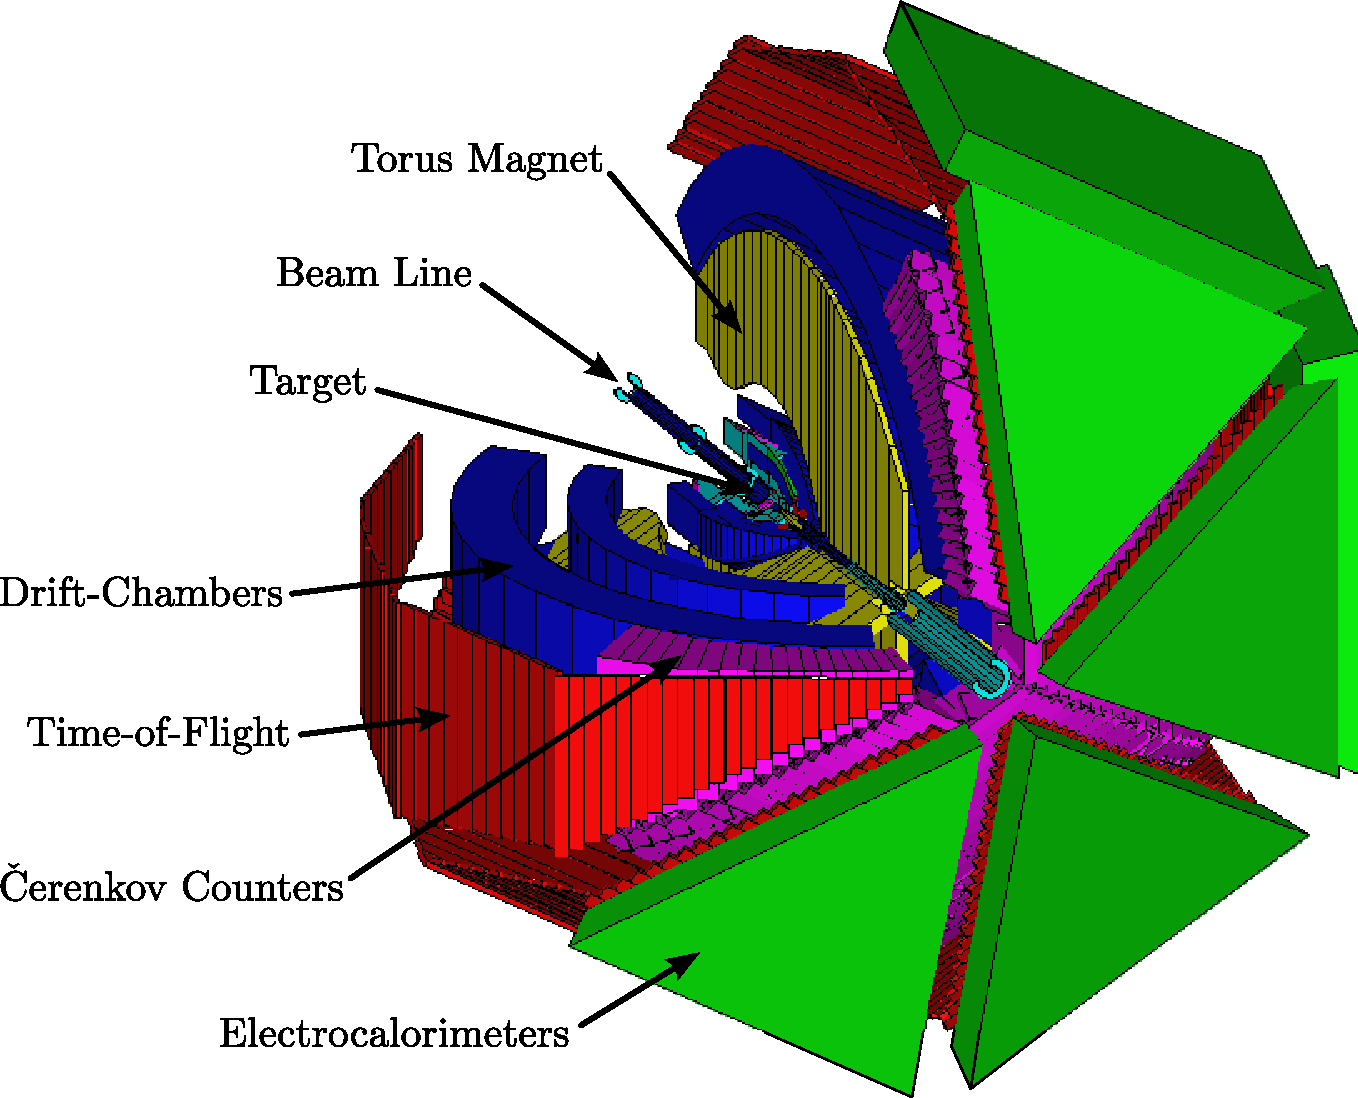
\includegraphics[width=0.8\columnwidth,height=\hfigheight]{\grpath/hall-b/clas_schematic.pdf}
\caption[\abbr{CLAS} Detector]{\label{fig:clas}{\coloronline}Schematic of the \abbr{CLAS} detector\cite{clas} with subsystems identified. This view is looking up-stream and the beam enters from the upper left. The detector is approximately 8~meters in diameter.}
\end{center}\end{figure}

\begin{figure}\begin{center}
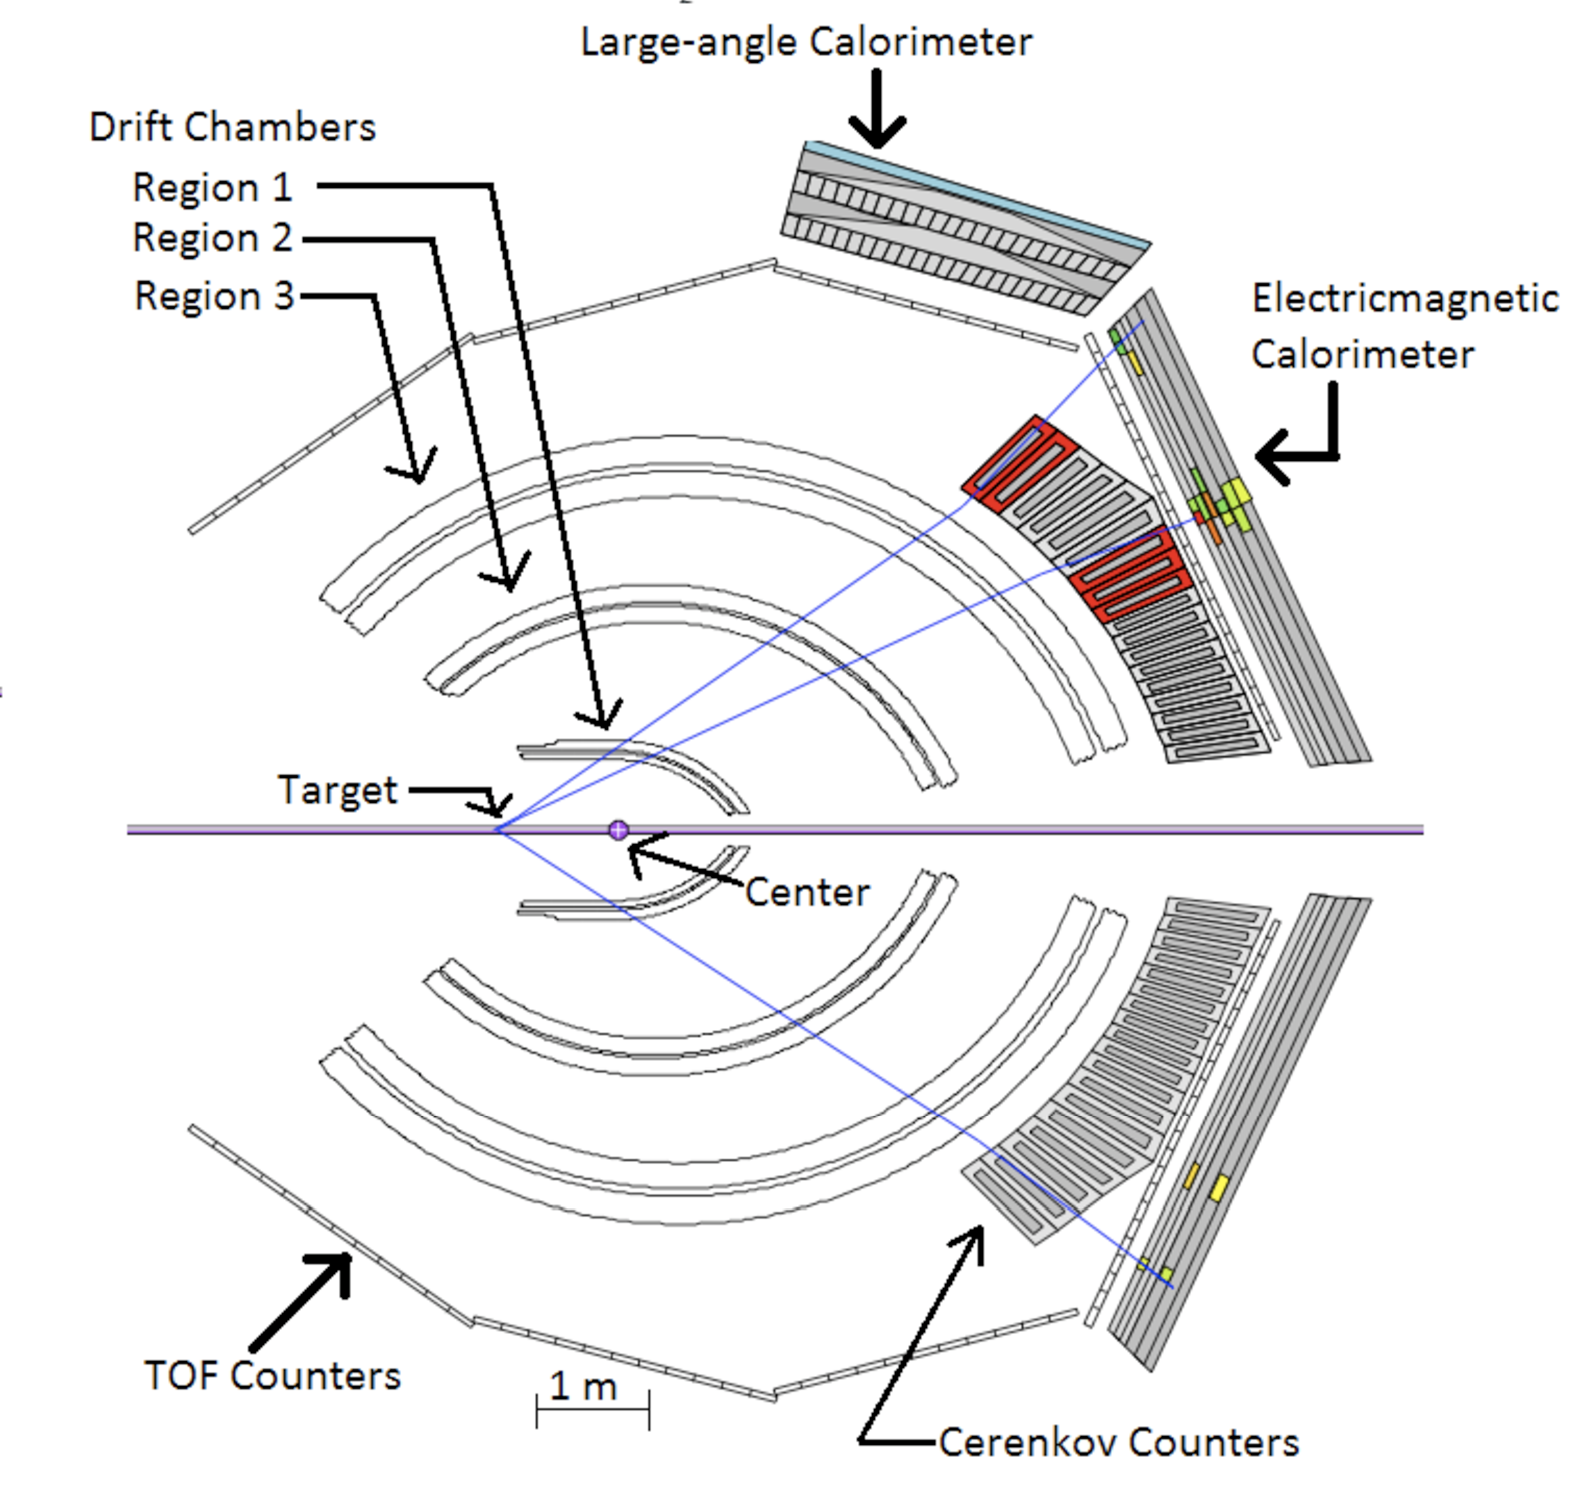
\includegraphics[width=0.6\columnwidth,height=\hfigheight]{\grpath/hall-b/clas_D.pdf}
\caption[\abbr{CLAS} Detector Diagram]{\label{fig:clas.ced}A cross section view of the \abbr{CLAS} detector showing an event with three tracks emanating from the target. The two tracks leaving hit patterns \abbr{CC} and \abbr{EC} are leptons while the track on the bottom panel is a proton}
\end{center}\end{figure}

\begin{figure}\begin{center}
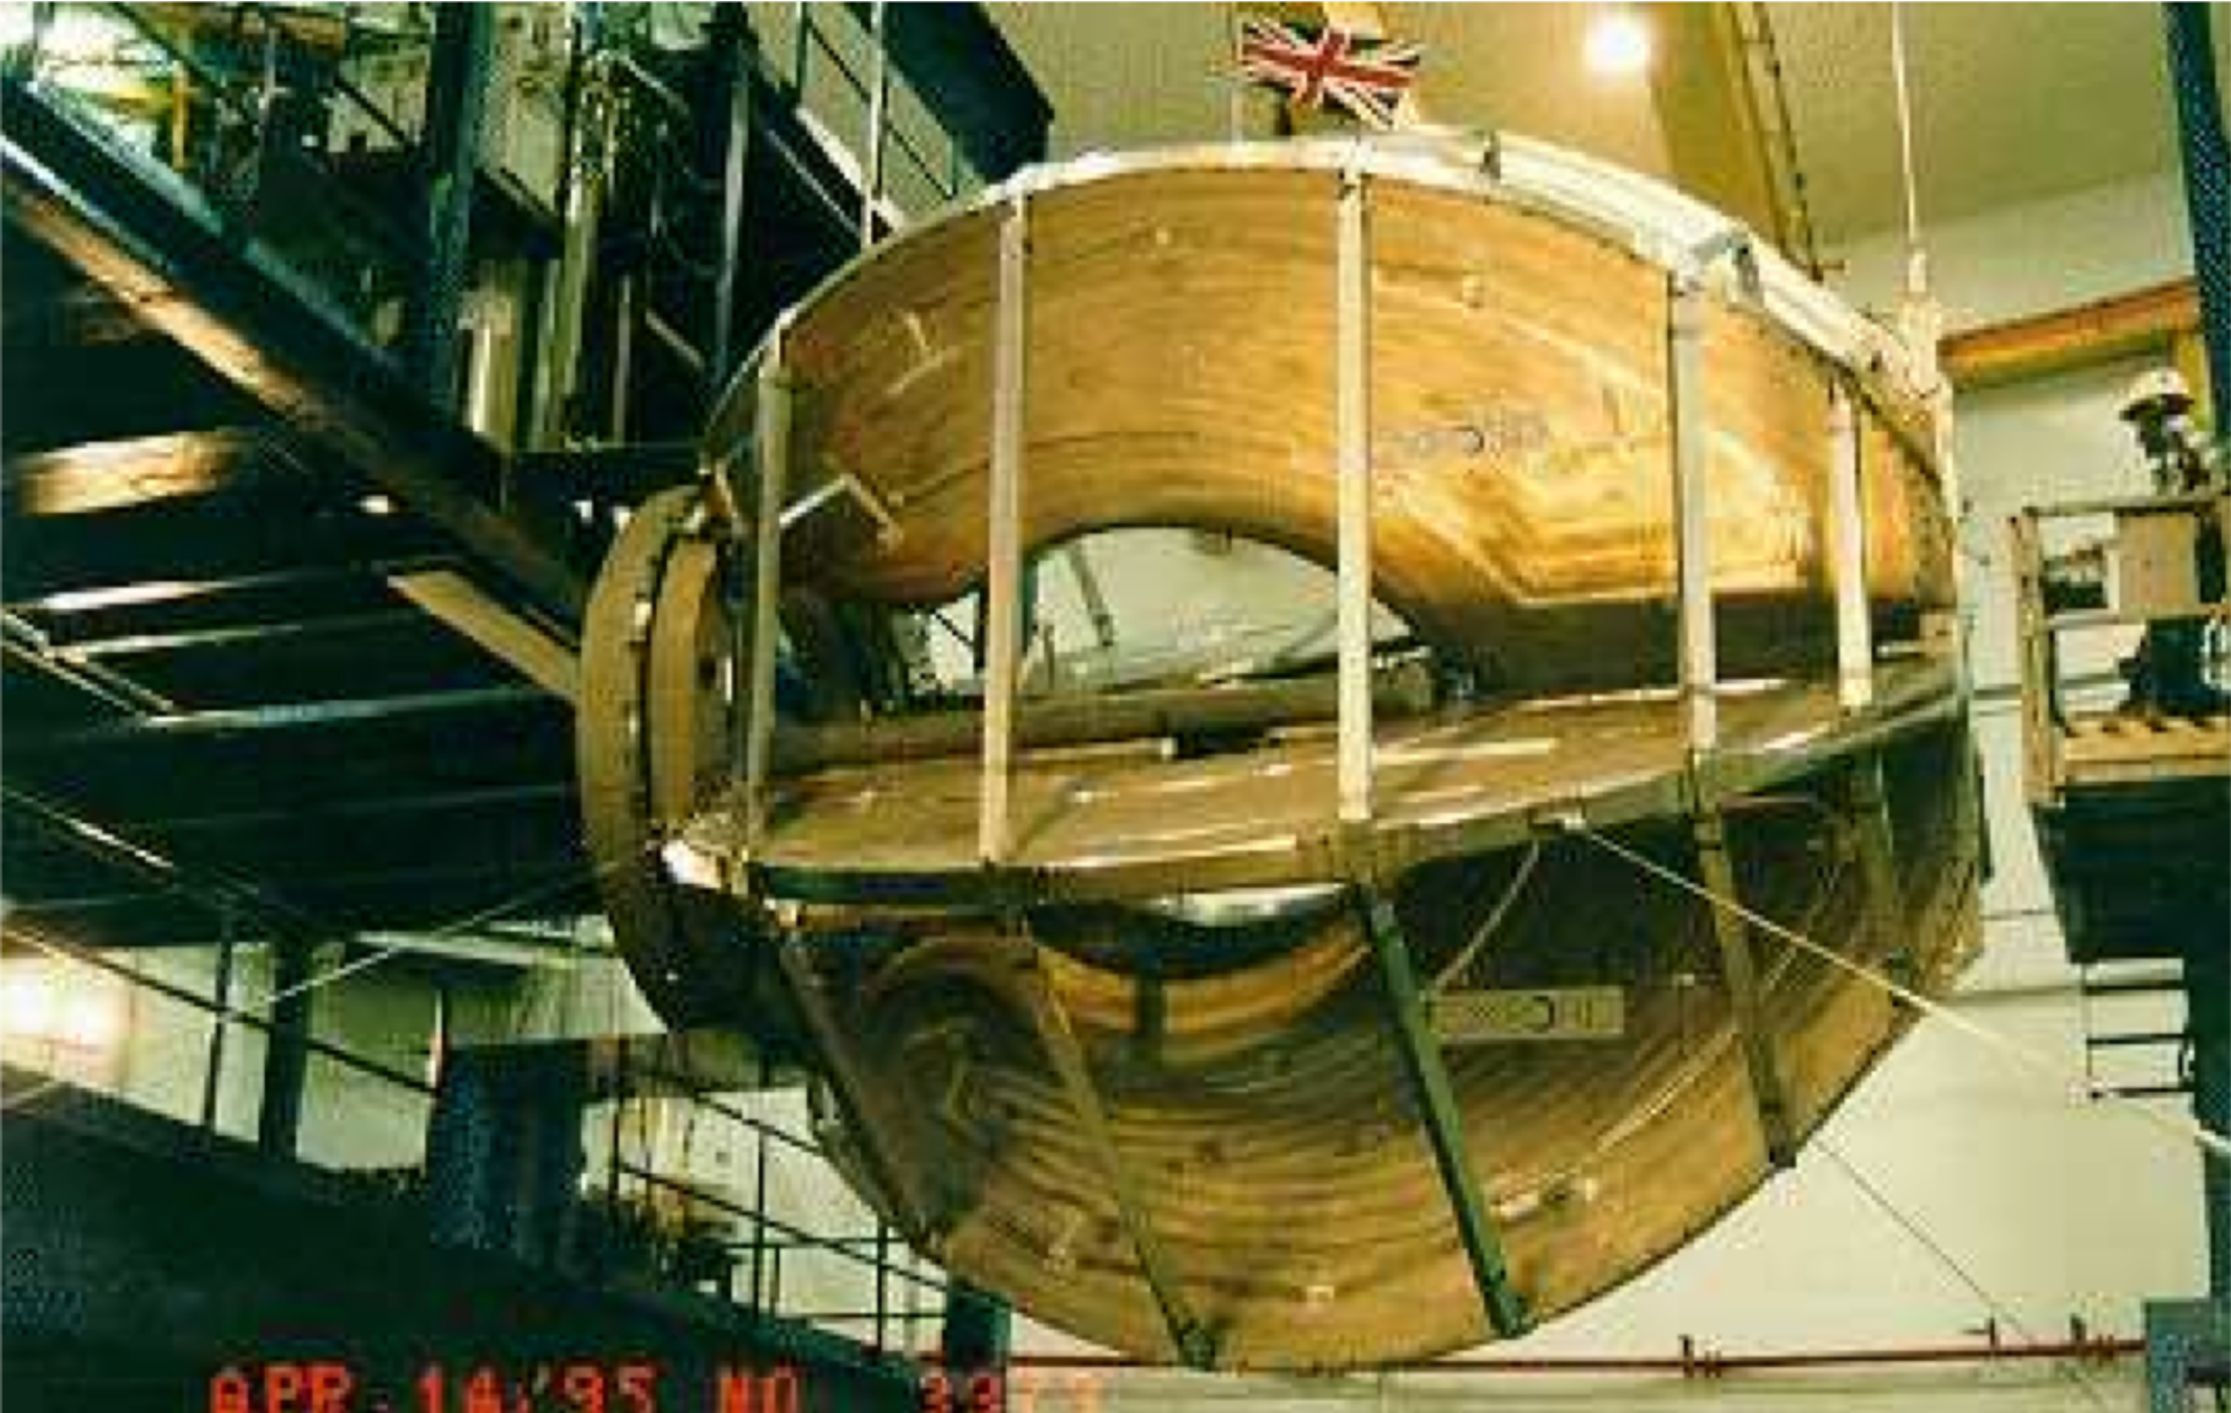
\includegraphics[width=0.8\columnwidth,height=\qfigheight]{\grpath/hall-b/torus_install.pdf}
\caption[Hall \abbr{B}]{\label{fig:torusinstall}{\coloronline}The coils of the \abbr{CLAS} toroidal magnet prior to installation of the rest of the detector. Image Source~\cite{williams}}
\end{center}\end{figure}


\subsection{Hydrogen Cryotarget}\label{sec:clas.tgt}


The target used by \g12 was conical as shown in Fig.~\ref{fig:clas.targetblueprint}. The target walls were constructed of 0.127~$\mu$m thick Kapton. It is 40~cm in length and 2~cm in radius. The incident photon beam had a radius of 1.5~cm. The target cell design shown in Figs,~\ref{fig:clas.targetblueprint} and~\ref{fig:clas.targetcell} had been used in several experiments and is capable of containing a number of different materials, such as helium, deuterium and hydrogen. For \g12 the target was filled with liquid hydrogen ($\ell$H$_2$). The temperature and pressure of the target was continuously measured and recorded. In Sec~\ref{sec:analysis.target_density}, these measurements will be used to calculate the density of the liquid Hydrogen to determine the target thickness. The target was not polarized.

\begin{figure}[h!]\begin{center}
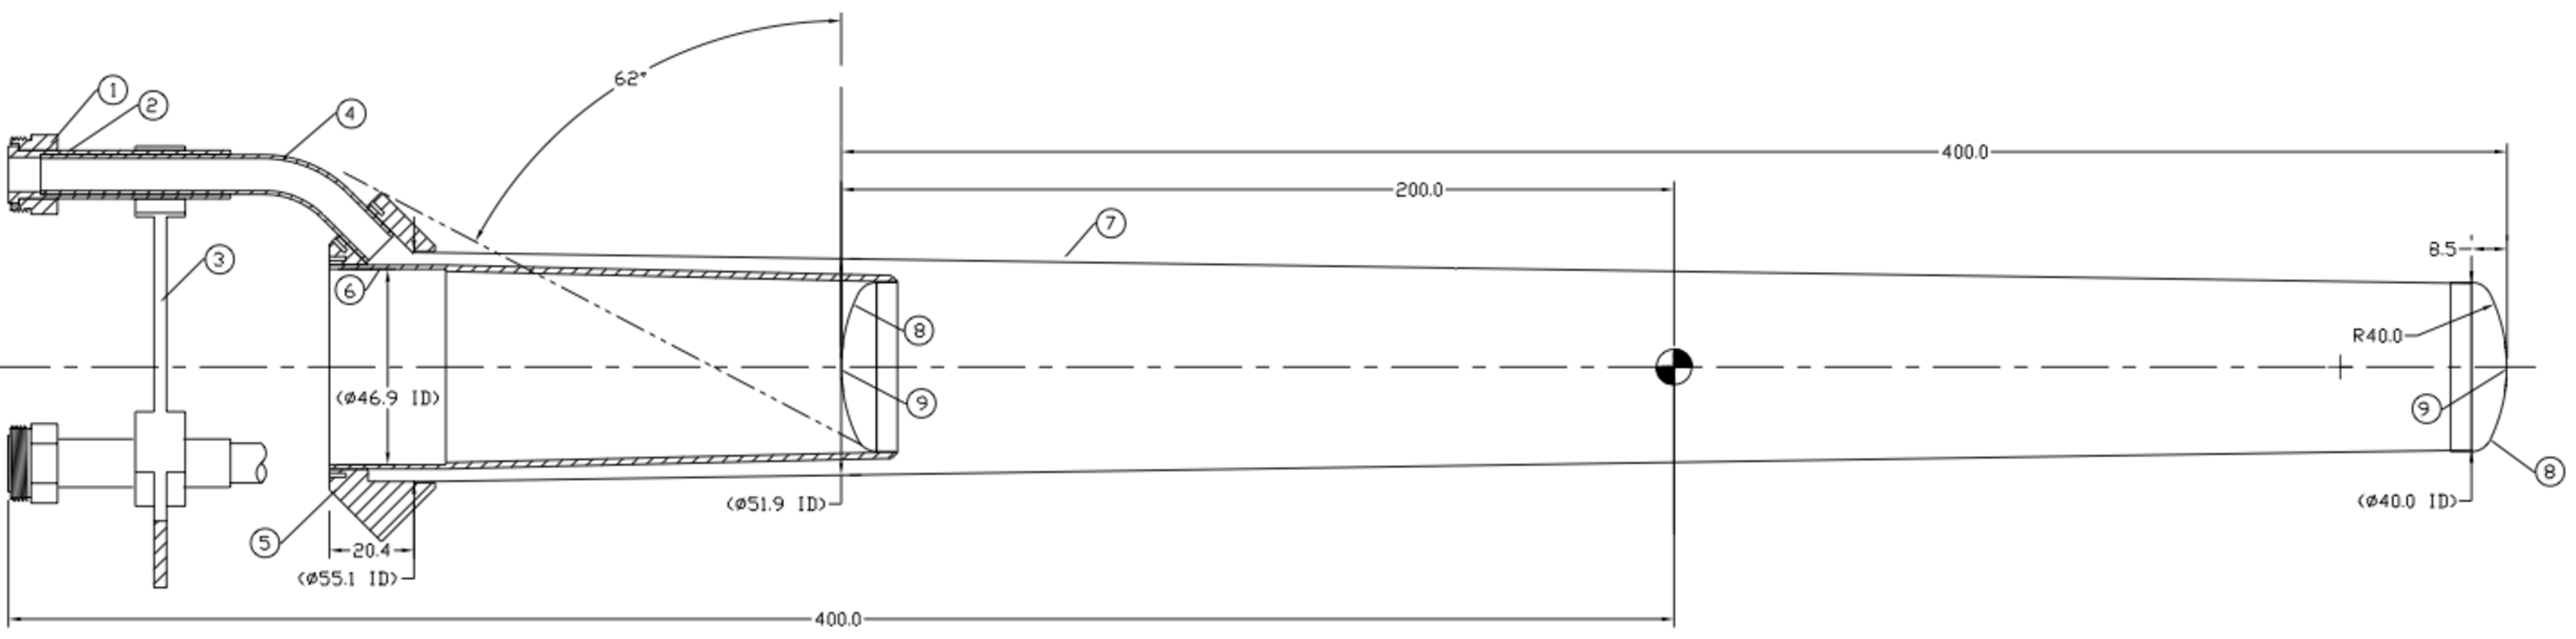
\includegraphics[width=\figwidth,height = \qfigheight]{\grpath/hall-b/g11_target_cell_blueprint.pdf}
\caption[Blueprint schematic of the conical Kapton target cell used for \g12]{\label{fig:clas.targetblueprint}Blueprint schematic of the conical Kapton target cell used for \g12.}
\end{center}\end{figure}

\begin{figure}[h!]\begin{center}
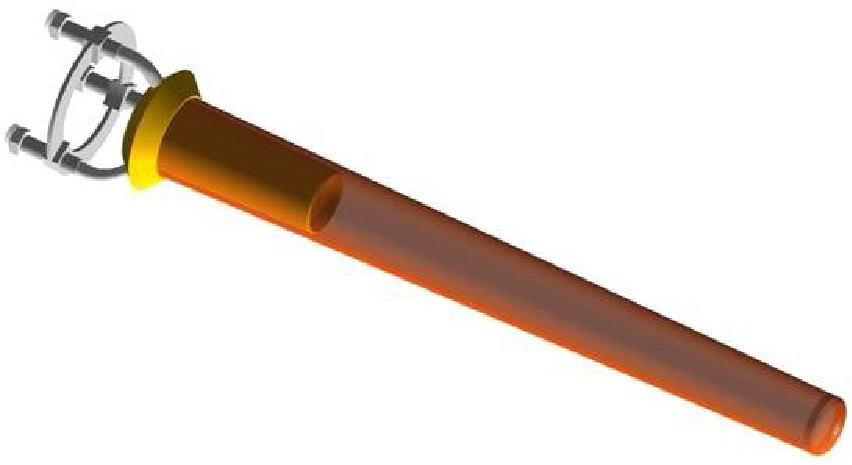
\includegraphics[width=0.6\figwidth]{\grpath/hall-b/g11_target_cell.pdf}
\caption[The 40~cm long conical Kapton target cell used for \g12]{\label{fig:clas.targetcell}The 40~cm long conical Kapton target cell used for \g12.}
\end{center}\end{figure}

%\subsubsection{Target Position for \g12}\label{sec:clas.tgt.position}
The target was located 90~cm upstream of \abbr{CLAS} the center, see Fig.~\ref{fig:clas.ced}.
This increased the forward angle acceptance from 8$^\circ$  to 6$^\circ$. However, this also decreased the large angle acceptance from approximately 140$^\circ$ to 100$^\circ$ in the lab frame.
%This reduction in large angle acceptance sacrificed multi-particle final state events, where the final state particles were more than about 70$^\circ$ away from beamline.
%as well as a reduction in \abbr{DC} resolution. The \abbr{DC} resolution decrease was due to the oblique angle the tracks made with the detector planes.
\FloatBarrier
\section{Start Counter}\label{sec:clas.st}

The start counter, Figs.~\ref{fig:clas.st} and~\ref{fig:clas.stxsection}, is a \abbr{PMT}-instrumented scintillator detector that surrounds the CLAS cryotarget hermetically. It consists of 24 scintillation paddles divided into six sectors matching that of \abbr{CLAS}. Each sector of the start counter is constructed of four independently-instrumented scintillator strips. Timing resolution of the start counter is $\sim$350~ps. The start counter information was used the \g12 triggers~\ref{sec.data.trig.lepton}. More information on the CLAS start counter can be found in \cite{clas.st}.

\begin{figure}[h!]\begin{center}
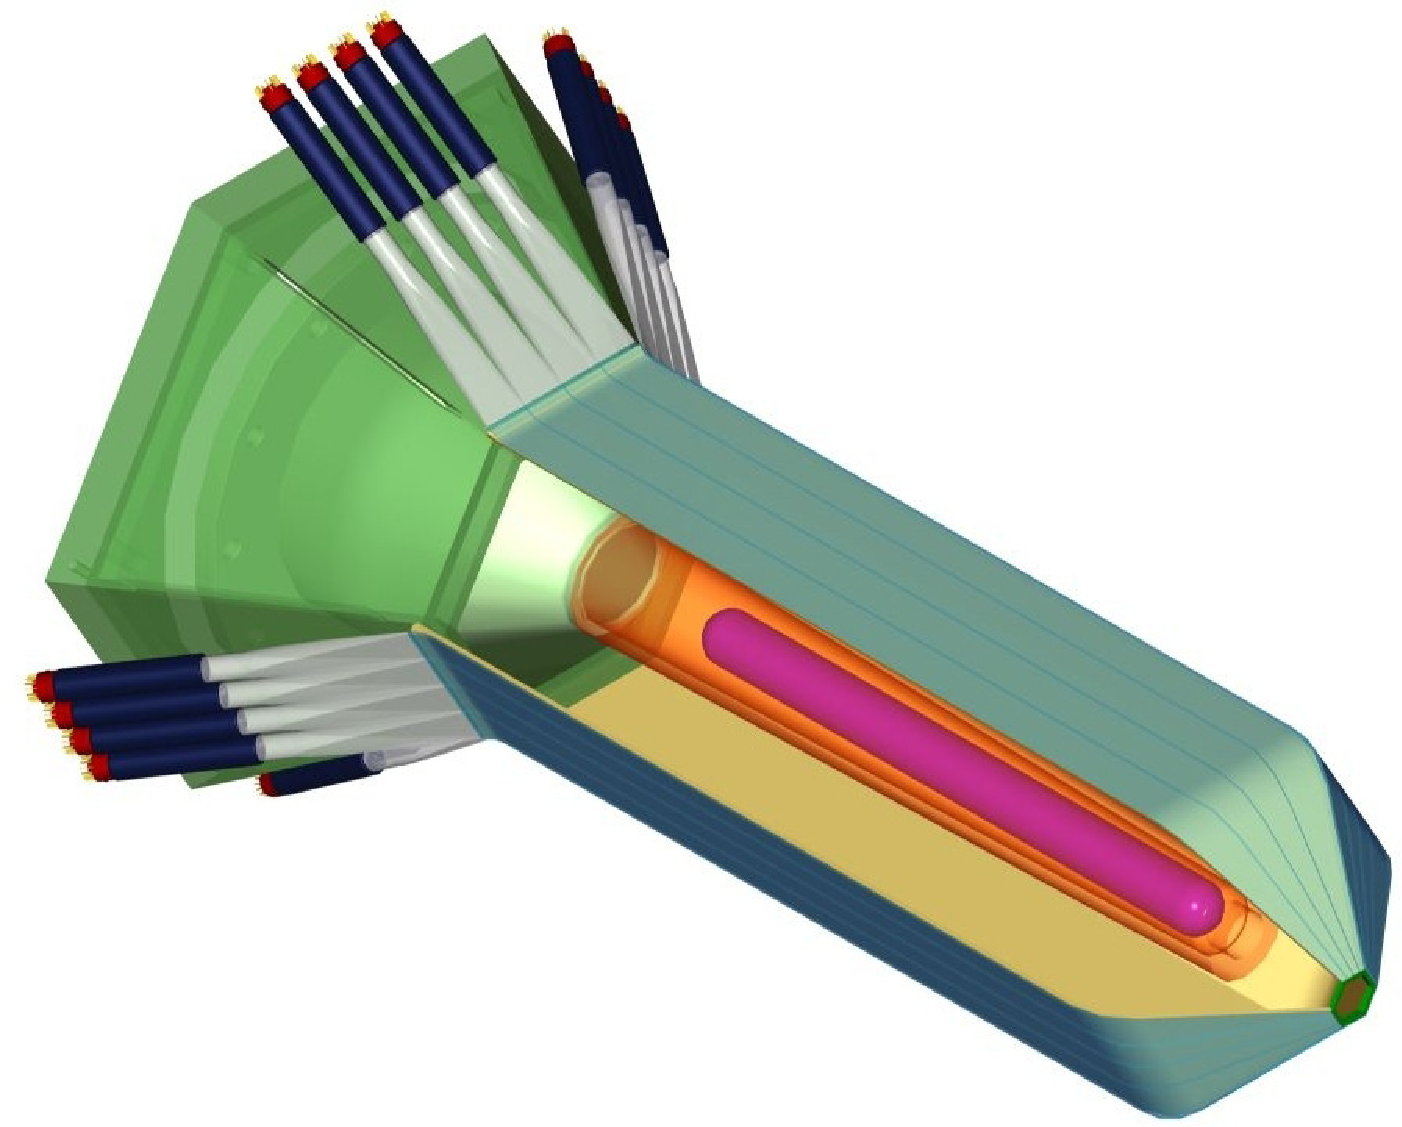
\includegraphics[width=0.8\figwidth,height=\qfigheight]{\grpath/hall-b/start_counter.pdf}
\caption[Schematic of the start counter (\abbr{ST}) with the 40~cm long target cell (purple) at the center]{\label{fig:clas.st}{\coloronline}Schematic of the start counter (\abbr{ST}) with the 40~cm long target cell (purple) at the center. The beam enters from the upper left of the figure.}
\end{center}\end{figure}

\begin{figure}[h!]\begin{center}
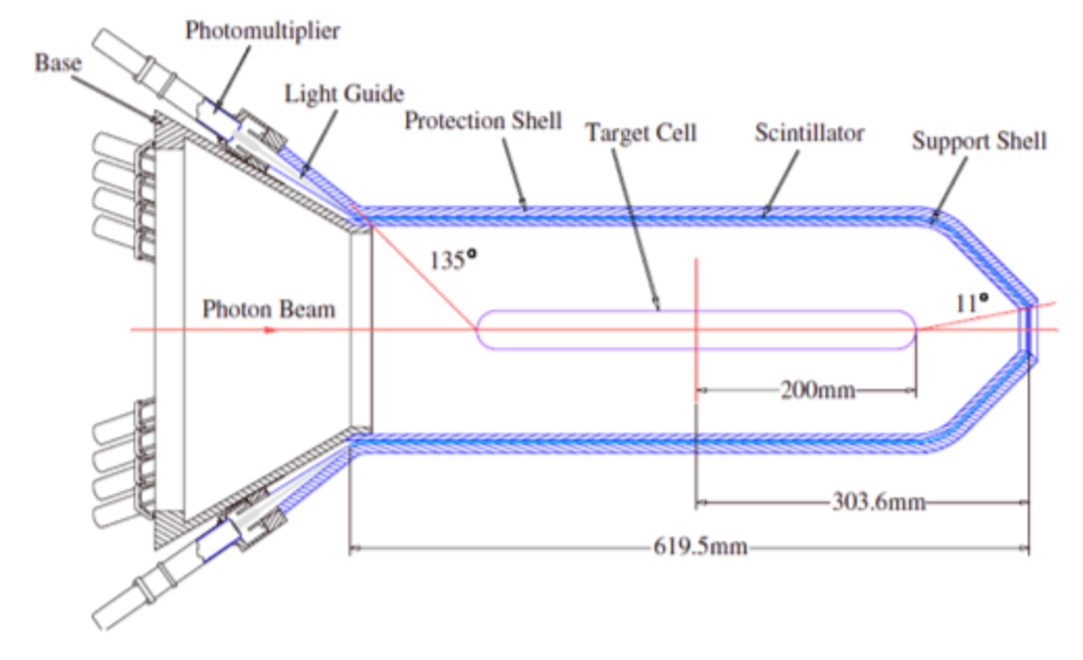
\includegraphics[width=0.8\figwidth,height=\qfigheight]{\grpath/hall-b/start_counter_wtarget.pdf}
\caption[Cross-section view of the start counter illustrating the labeled components and its angular coverage when at the center of \abbr{CLAS}]{\label{fig:clas.stxsection}{\coloronline}Cross-section view of the start counter illustrating the labeled components and its angular coverage when at the center of \abbr{CLAS}.}
\end{center}\end{figure}

\FloatBarrier
%\subsection{Start Counter Efficiency Analysis}\label{sec:clas.st.eff}
%There is an inefficiency of the start counter as seen in Fig.~\ref{fig:classt.ineff}. This inefficiency was measured by using real data events as generated events and passing them through \abbr{CLAS}'s Monete-Carlo package(\abbr{GSIM}\label{abbr:gsim}). More information about this inefficiency will be discussed in Sec.~\ref{sec:analysis.accept.verify}.
%
%%It was observed that 20~\% of the events would fail in simulation, this will be discussed in Sec~\ref{sec:gsim.efficiency}. A portion of the failed events were based upon a failure to reconstruct the required banks for the start counter. This phenomena was investigated from the raw data and found to also be present in the processing of the data from raw to user file in the same manner as seen from Monte-Carlo. The blue-dashed line in Fig.~\ref{fig:classt.ineff} illustrates the start counter inefficiency that is dependent on the events reconstructed vertex. The inefficiency is due to the start counter reconstruction algorithm not being able to link the start counter hit to a track through time-based tracking. This track is not lost due to a reprocess of time-based tracking, linking the track to another particles start counter hit with the same 
%
%%The inefficiency of the start counter is not a mechanical fault but rather the fault of the algorithm used to reconstruct a start counter hit. TO study this raw data events were processed event by event using the program DDD and \abbr{CLAS} event display (\abbr{ced}). Unknown of the cause, it  
%
%
%\begin{figure}[h!]\begin{center}
%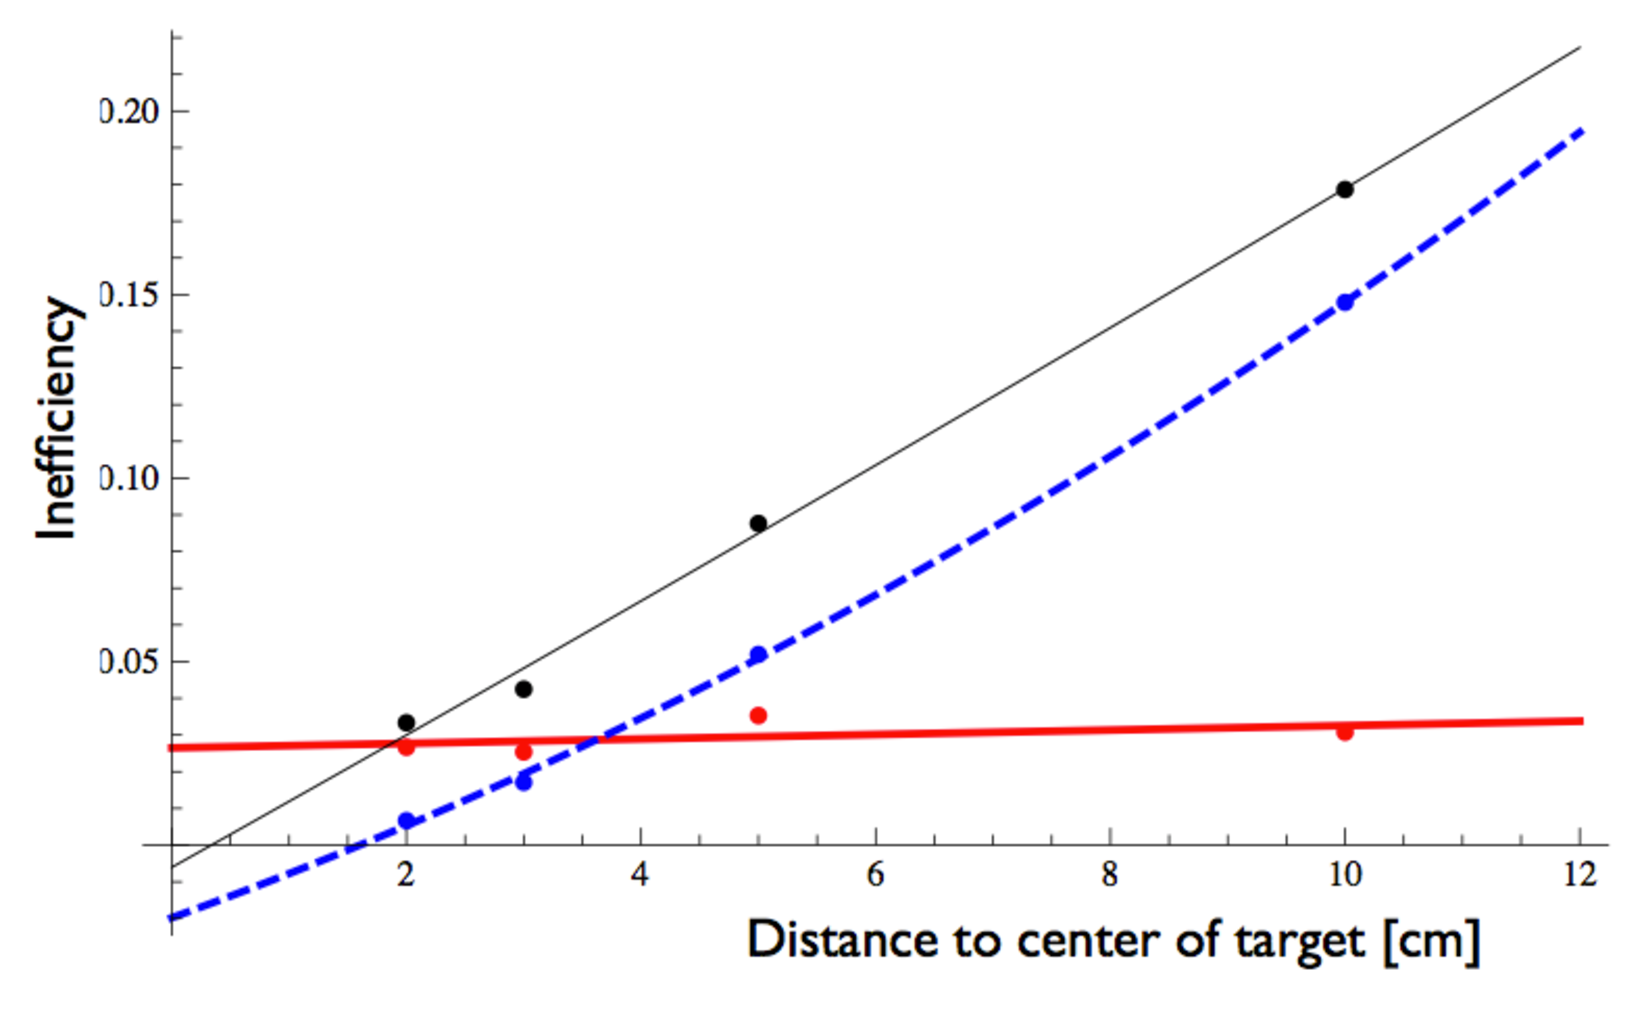
\includegraphics[width=0.8\figwidth,height=0.7\hfigheight]{\grpath/hall-b/st_issue_4_thesis.pdf}
%\caption[Start Counter Inefficiency]{\label{fig:classt.ineff}{\coloronline}Plot showing the inefficiency of the start counter from data events, red-solid line is the inefficiency of reconstruction based solely on hit-based tracking, blue-dashed line is inefficiency of start counter, black-solid is combined. }
%\end{center}\end{figure}
%
%\FloatBarrier
\section{Superconducting Toroidal Magnet}\label{sec:clas.tor}

The essence of \abbr{CLAS} is the use of a toroidal magnetic field generated by six superconducting coils consisting of 4 layers of 54 windings of aluminum-stabilized niobium titanium NbTi/Cu superconductor \cite{clas}. The coils are separated in the azimuthal direction, $\phi$, by 60$^\circ$ and are located between Region-1 and Region-3 of the \abbr{DC}, see Fig~\ref{fig:clas.dc.torus.mag}. The placement of the coils is such that the magnetic field is encompassed by the volume of the \abbr{DC}, see Fig.~\ref{fig:clas.dc.torus.mag}. The direction of the toroidal field points along $\phi$, except near the coils,  such that the charged particles conserve their azimuthal angle along their trajectory, see Fig~\ref{fig:clas.dc.torus.cont}. The maximum current the magnet can support is 3861~A, resulting in a maximum field strength of 35~kG. During the \g12 experiment, the magnets operated at a current of 1930~A corresponding to a maximum field of about 20~kG. The field was oriented such that positive charged particles bent away from the beam-line, while negative charged particles bent toward the beam-line. Running at higher currents provides better momentum resolution but decreases the detector's acceptance for negative particles. Knowing the strength and direction of the magnetic field and the trajectory of a particle using the \abbr{DC}, the particle momentum can be determined by use of Eq.~\ref{eq:motioninmag}.
% During the \g12 experiment, the magnet was cooled down to 4.5~K using liquid helium ($\ell$He) obtained from the central CEBAF central cryogenic facility.

\begin{figure}[h!]\begin{center}
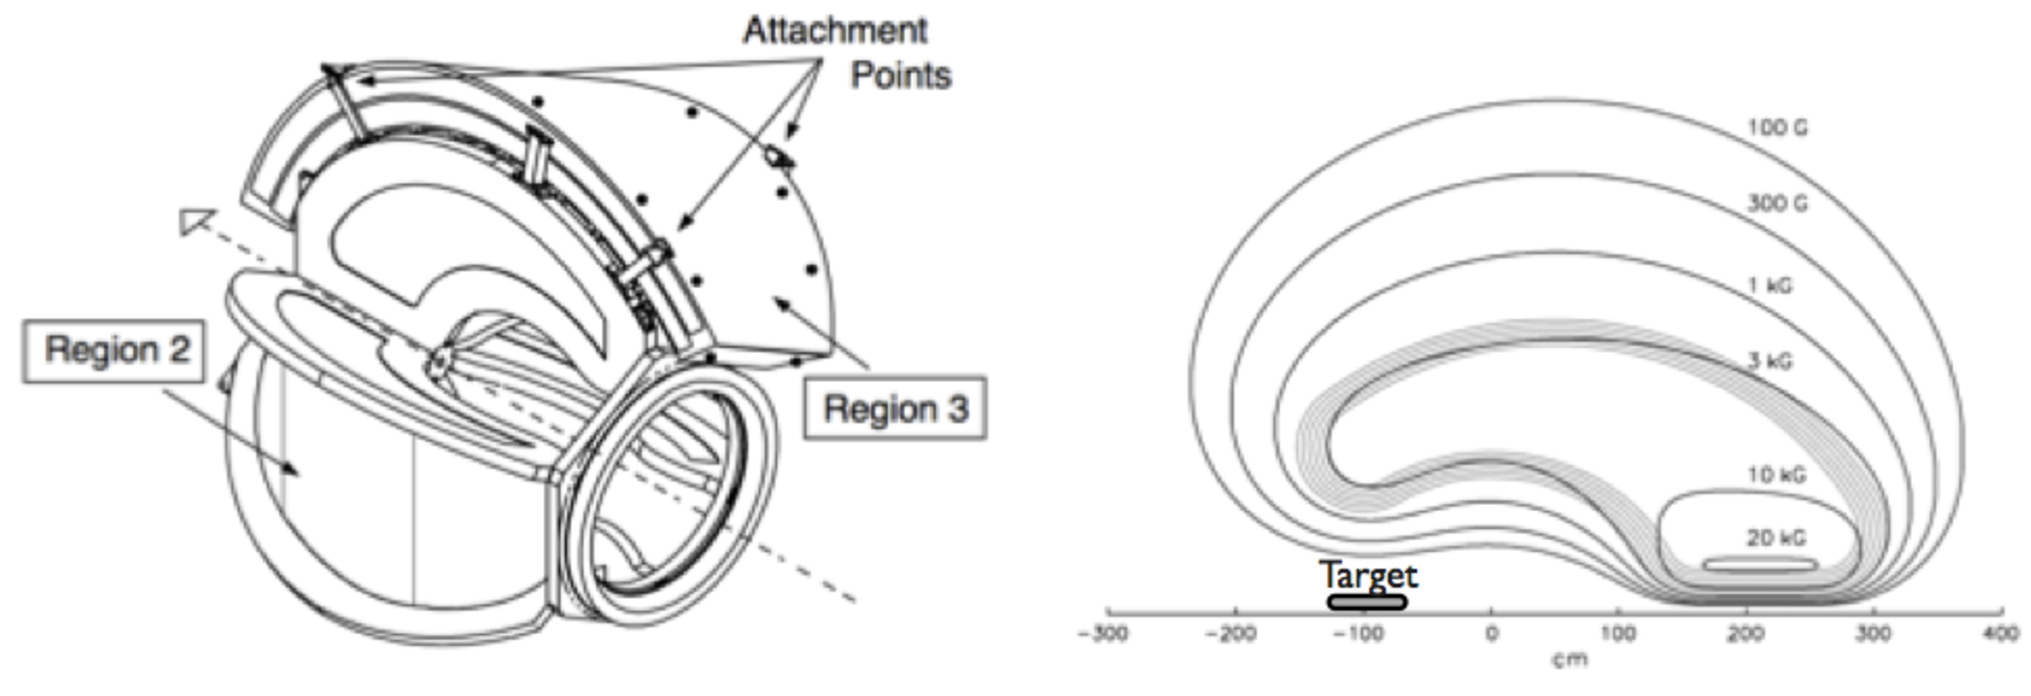
\includegraphics[width=\figwidth,height=0.9\qfigheight]{\figures/hall-b/torus_field_mag_mount.pdf}
\caption[The \abbr{CLAS} Superconducting Toroidal Magnet and its placement in relation to Region-1 and Region-3]{\label{fig:clas.dc.torus.mag}The \abbr{CLAS} Superconducting Toroidal Magnet and its placement in relation to Region-1 and Region-3  (left). Cross-section of the \abbr{CLAS} Superconducting Toroidal Magnet at half current (1930~A). Region-2 of the \abbr{DC} is located inside the region of the coils shown as the kidney shaped loop at about 3~kG (right).}
\end{center}\end{figure}

\begin{figure}[h!]\begin{center}
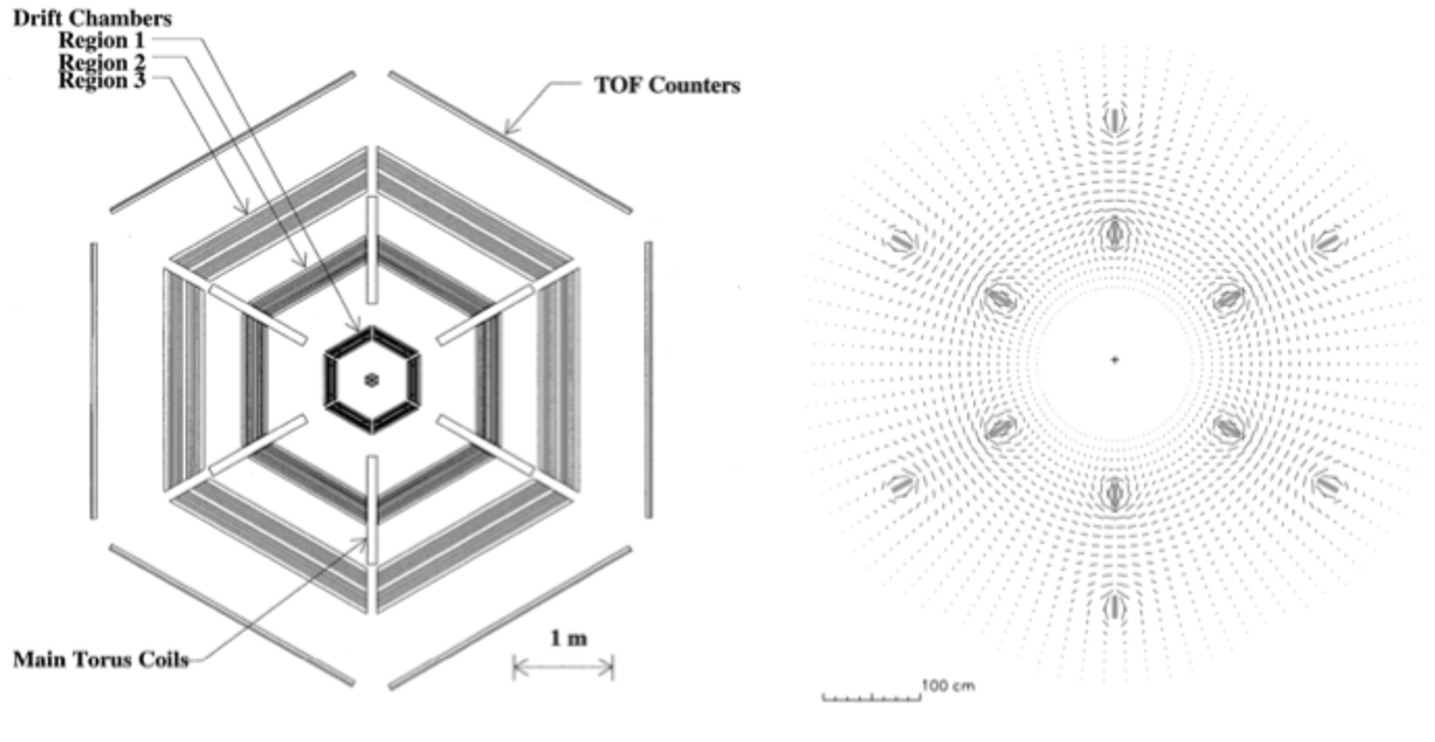
\includegraphics[width=1.\figwidth,height=0.75\hfigheight]{\figures/hall-b/torus_field_and_DC.pdf}
\caption[Schematic cross-sectional view of the \abbr{CLAS} detector, perpendicular to the beam line]{\label{fig:clas.dc.torus.cont}Schematic cross-sectional view of the \abbr{CLAS} detector, perpendicular to the beam line (left). The magnetic field distribution corresponding to the view in the left figure. The field is purely azimuthal. The six torus coils are shown in grey, the field is in the counter-clockwise direction,  the field strength is concentrated in the region between the coils (right).}
\end{center}\end{figure}

\FloatBarrier
\section{Drift Chambers}\label{sec:clas.dc}

The \abbr{CLAS} drift chambers \abbr{DC} (Figs.~\ref{fig:clas},~\ref{fig:clas.dc.torus.cont},~\ref{fig:clas.dc.drift}) track charged particles above 200~MeV/c with polar angle resolution of 2-4~mrad and momentum resolution of 0.5 - 1\%, depending on momentum, see Fig~\ref{fig:clas.dc.res}. Typical coverage of the \abbr{DC} is $8^\circ < \theta < 142^\circ$, when the target is at \abbr{CLAS} center. For the \g12 experiment the coverage of the \abbr{DC} was modified to $6^\circ < \theta < 100^\circ$ due to the placement of the target, see Sec~\ref{sec:clas.tgt} for reasons explained in ~\cite{clas.proposal.hyclas},~\cite{clas.proposal.superg},~\cite{clas.proposal.pion}.
\begin{figure}\begin{center}
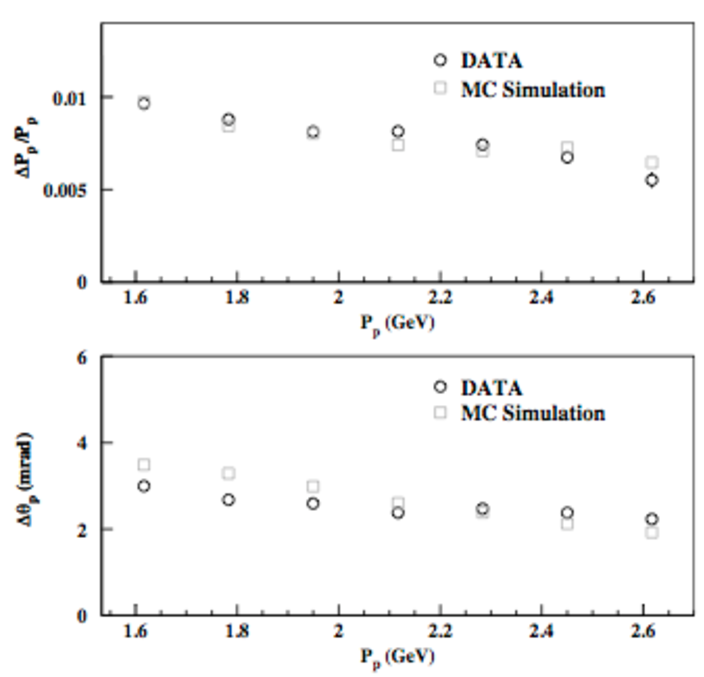
\includegraphics[width=0.8\figwidth,height=0.75\hfigheight]{\figures/hall-b/drift_DC_resolution.pdf}
\caption[Momentum and angular resolution for protons as determined from the measured angle of the scattered electron for data collected and Monte-Carlo simulation]{\label{fig:clas.dc.res}Momentum and angular resolution for protons as determined from the measured angle of the scattered electron for data collected and Monte-Carlo simulation. Image Source~\cite{clas}}
\end{center}\end{figure}

The \abbr{DC} are divided into six sectors each containing three radial layers (Fig.~\ref{fig:clas.dc.drift}), referred to as ``Regions'', for a total of 18 separate drift chambers. Each \abbr{DC} region covers the same polar angular range and consist of two superlayers which each contain six layers of hexagonal wire cells which house evenly spaced 20~$\mu$m gold-plated tungsten sense wires (center of hexagon) each surrounded by six 140~$\mu$m gold-plated aluminum alloy field wires (vertices of hexagon). In the first superlayer, the wires are strung approximately parallel to the direction of the magnetic field (axial wires), while the second superlayer has wires tilted at a 6$^\circ$ angle with respect to the axial wires (stereo wires). A high voltage system maintains the sense wires at positive potential, while the field wires are maintained at a negative potential 50\% lower than the positive value. The difference of potentials creates an avalanche of the electrons induced by the ionizing particle. The hexagonal shape of the cell mimics a circular geometry cell in which the drift time to drift distance is independent of entrance angle.

The inner region is denoted as Region 1. Its first superlayer has only 4 layers due to space constraints. Region 1 is nearly free from magnetic field, see Fig~\ref{fig:clas.dc.torus.mag}. Region 2 is situated between the magnetic coils which is subject to the highest magnetic field which is used to determine the particle's curvature, needed to determine the particle;s momenta, see Eq.~\ref{eq:motioninmag}. Region 3 purpose is to provide global track reconstruction in connection with other CLAS detectors since Region 3 is located outside the volume of magnetic field. Each \abbr{DC} is filled with a gas mixture of 90\% argon and 10\% carbon-dioxide. This choice of gas provides high drift velocity (0.04 m/$\mu$sec) and fast collection time which improves momentum resolution. For more information on the design of the \abbr{CLAS} \abbr{DC} system, see~\cite{clas.dc} and for more information on the calibration process of the \abbr{CLAS} \abbr{DC} system, see~\cite{clas.dc.calib}.

\begin{figure}\begin{center}
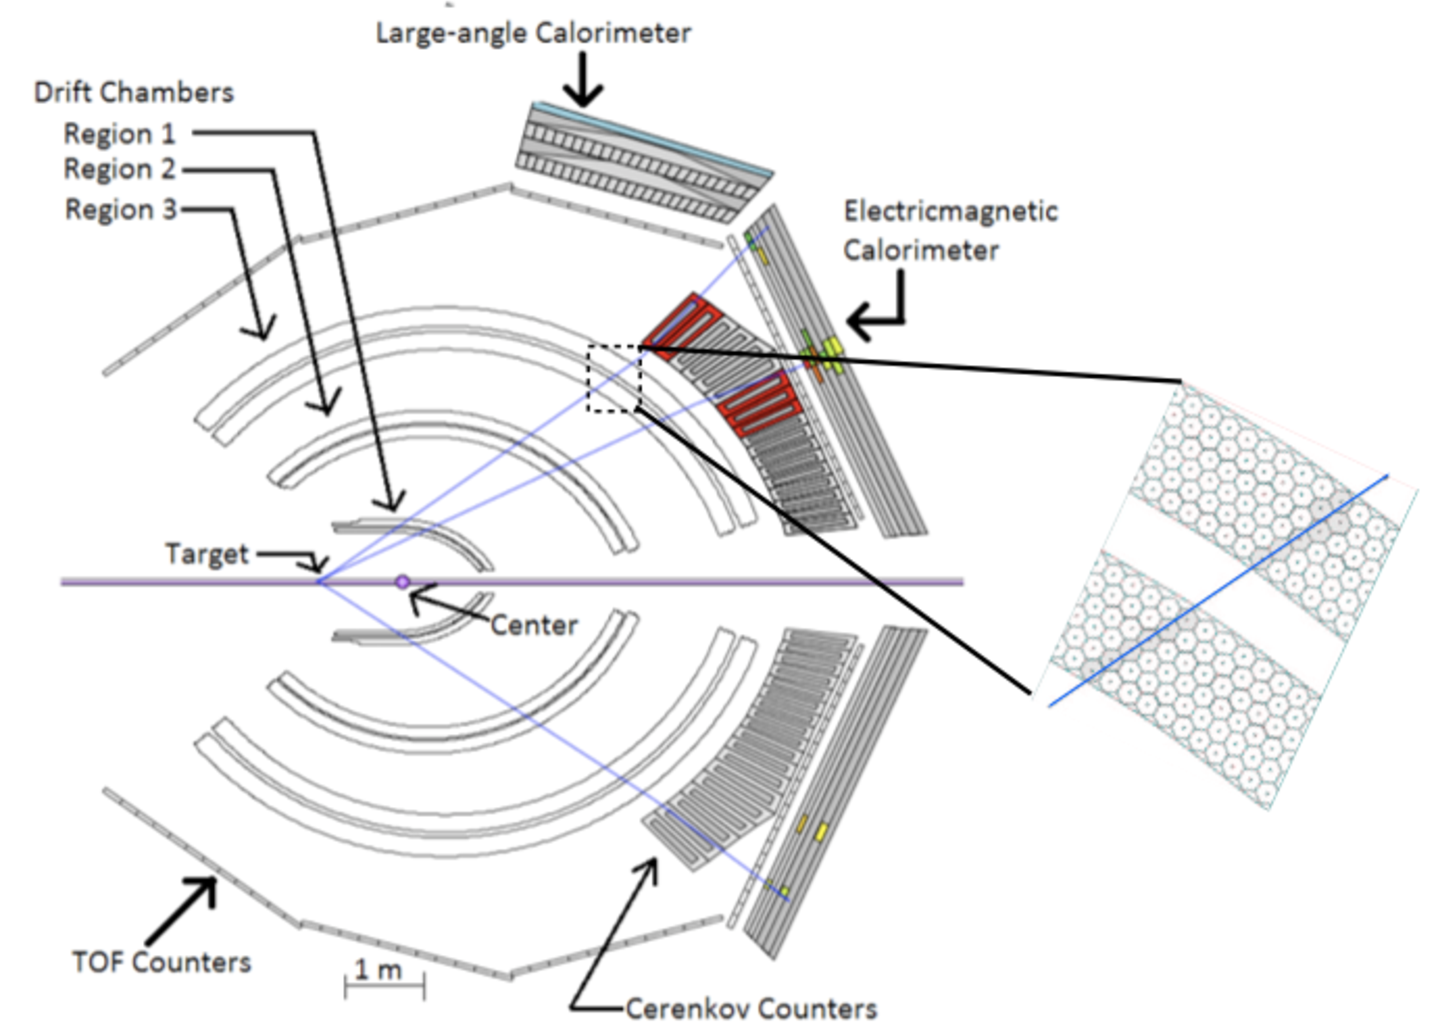
\includegraphics[width=\figwidth,height=0.75\hfigheight]{\figures/hall-b/drift_DC_cedII.pdf}
\caption[A cross section view of the \abbr{CLAS} detector showing an event with three tracks emanating from the target]{\label{fig:clas.dc.drift}A cross section view of the \abbr{CLAS} detector showing an event with three tracks emanating from the target. The two tracks leaving hit patterns \abbr{CC} and \abbr{EC} are leptons while the track on the bottom panel is a proton. The inlet shows hexagonal cells of drift chambers with a typical track indicated by shaded areas for the cut-out in Region-3.}
\end{center}\end{figure}

\FloatBarrier
\section{Time-of-Flight Detectors}\label{sec:clas.tof}

The \abbr{CLAS} time-of-flight \abbr{TOF} subsystem provides precise timing measurements of charged particles that transverse the \abbr{CLAS} detector to help determine the particle masses. The \abbr{TOF} subsystem was also used in the \g12 level 1 trigger (see Sec.~\ref{sec:data.trig}) to identify track candidates. The \abbr{TOF} is constructed of organic plastic scintillant (Bicron BC-408). Scintillation is a process undergone by material when radiation traverses a medium.
%
% At room temperature, all valence electrons of the scintillating material are in the $\mathrm{S_{0}}$ ground state. As a particle propagates through the material the incident radiation populates $\mathrm{S_{1}}$ states. Vibrational levels within $\mathrm{S_{1}}$ band decay radiation-less to $\mathrm{S_{1}}$  base states, which in turn decays under emission of light to the $\mathrm{S_{0}}$ band. The radiation-less decay from the excited $\mathrm{S_{1}}$ band to the ground $\mathrm{S_{1}}$ band is known as internal degradation and is responsible for the transparency of the scintillators to their own radiation. $\mathrm{S_{1}}$ can also decay to adjacent triplet levels however, this decay is highly forbidden by multipole selection rules. If this decay does occur, the decay energy is lower causing the decay time to be longer, see Fig.~\ref{fig:clas.scint_bands} for the illustration of this process. Depending on the properties of the scintillator, decay of fluorescent state in organic plastic scintillators have a typical time between 1-3~ns
%
%%\begin{figure}[h!]\begin{center}
%%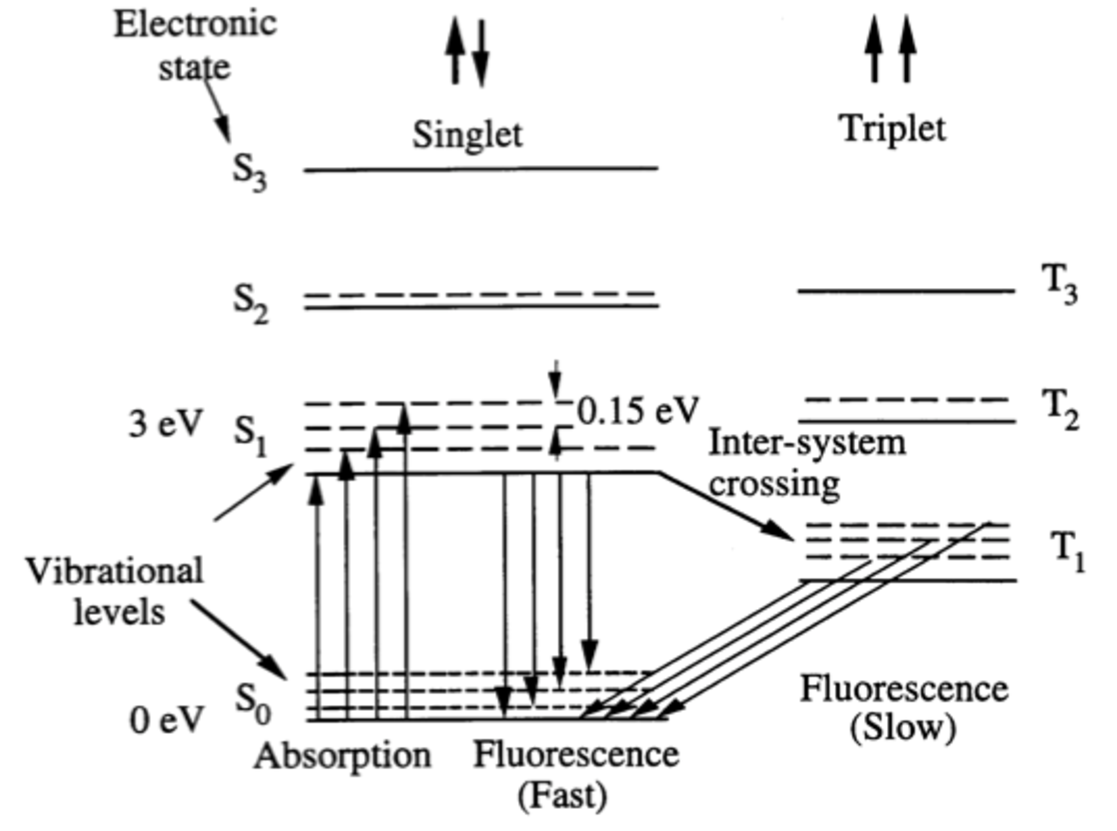
\includegraphics[width=\figwidth,height=0.5\hfigheight]{\figures/hall-b/CCECPLOTS/Calorimetry/scint.pdf}\label{fig:clas.scint_bands}\caption[Typical Energy Levels of scintillating material ]{Diagram of scintillating population of states. Image Source~\cite{vibe_levels}}
%%\end{center}\end{figure}
%\begin{figure}[h!]\begin{center}
%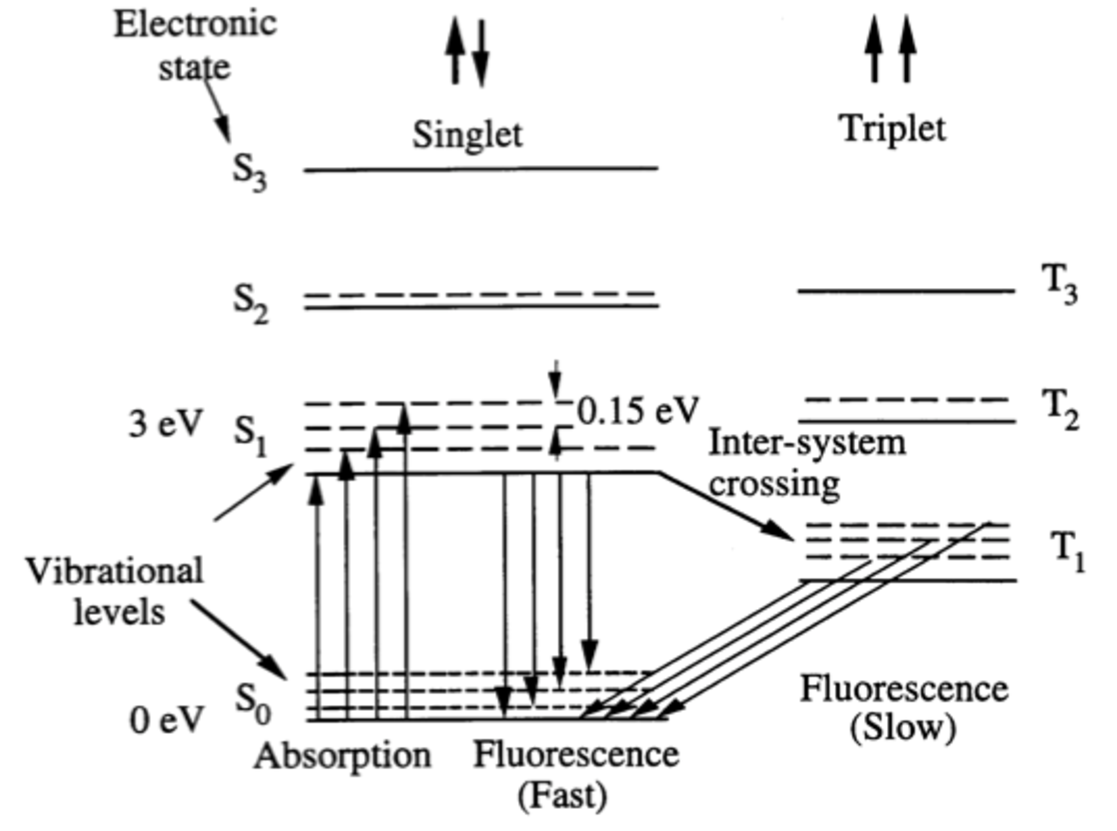
\includegraphics[width=\figwidth,height=0.5\hfigheight]{\figures/hall-b/CCECPLOTS/Calorimetry/scint.pdf}
%\caption[Typical Energy Levels of scintillating material ]{\label{fig:clas.scint_bands}Diagram of scintillating population of states. Image Source~\cite{vibe_levels}}
%\end{center}\end{figure}

The \abbr{TOF} subsystem is located between the \abbr{CC} and \abbr{EC} subsystems approximately 4~m from \abbr{CLAS} center, 5~m from the \g12 target. Each sector 57 scintillator paddles divided into two subgroups. The first subgroup subtends angles of 8.6$^\circ$ to 45.9$^\circ$ and consists of 23 scintillating paddles that are 15~cm in width. Each paddle is instrumented with two 2-in diameter \abbr{PMT}'s, see Fig~\ref{fig:clas.tof.paddles}. The first group was optimized for timing resolution while being cost-effective and covering a large area. The second group consists of 34 paddles that are 22~cm wide, covering polar angles from 45.9$^\circ$ to 142$^\circ$. Each paddle in this range is instrumented with two 3-in diameter \abbr{PMT}'s. All paddle bars are 5.08~cm thick for 100\% detection of minimum-ionizing tracks and a timing resolution of 150--200~ps.
%These forward angle counters \abbr{PMT}'s have a 15.9~cm$^2$ photocathode area which covers the 76.2~cm$^2$ cross-sectional area of the scintillator.
%These large angle counter \abbr{PMT}'s have a 30.2~cm$^2$ photocathode area which covers the 118.8~cm$^{\mathrm{2}}$ cross-sectional area of the scintillator.
\abbr{TOF} information is used to reconstruct a particle's mass is by measuring the difference between the event RF corrected start time and the time measured by the \abbr{TOF}, $t_{stsc}$. The RF corrected start time is the radio-frequency time (RF) from the accelerator beam aligned withe the event start time. Using this time, $t_{stsc}$, the length of trajectory to the \abbr{TOF}, $l_{stsc}$, and the speed of light $c$, the particles' velocity can be calculated as
\begin{equation}\label{eq:beta.cal}
\beta = l_{sc}/(t_{c}\cdot c)
\end{equation}
The particle's mass can be reconstructed from the measured velocity and momentum:
%Once the particles velocity is determined as well as the momentum, from the \abbr{DC} subsystem,  the particle mass can be reconstructed as 
\begin{equation}\label{eq:mass.cal}
m = p\sqrt{(1-\beta^2)}/\beta
\end{equation}

\begin{figure}\begin{center}
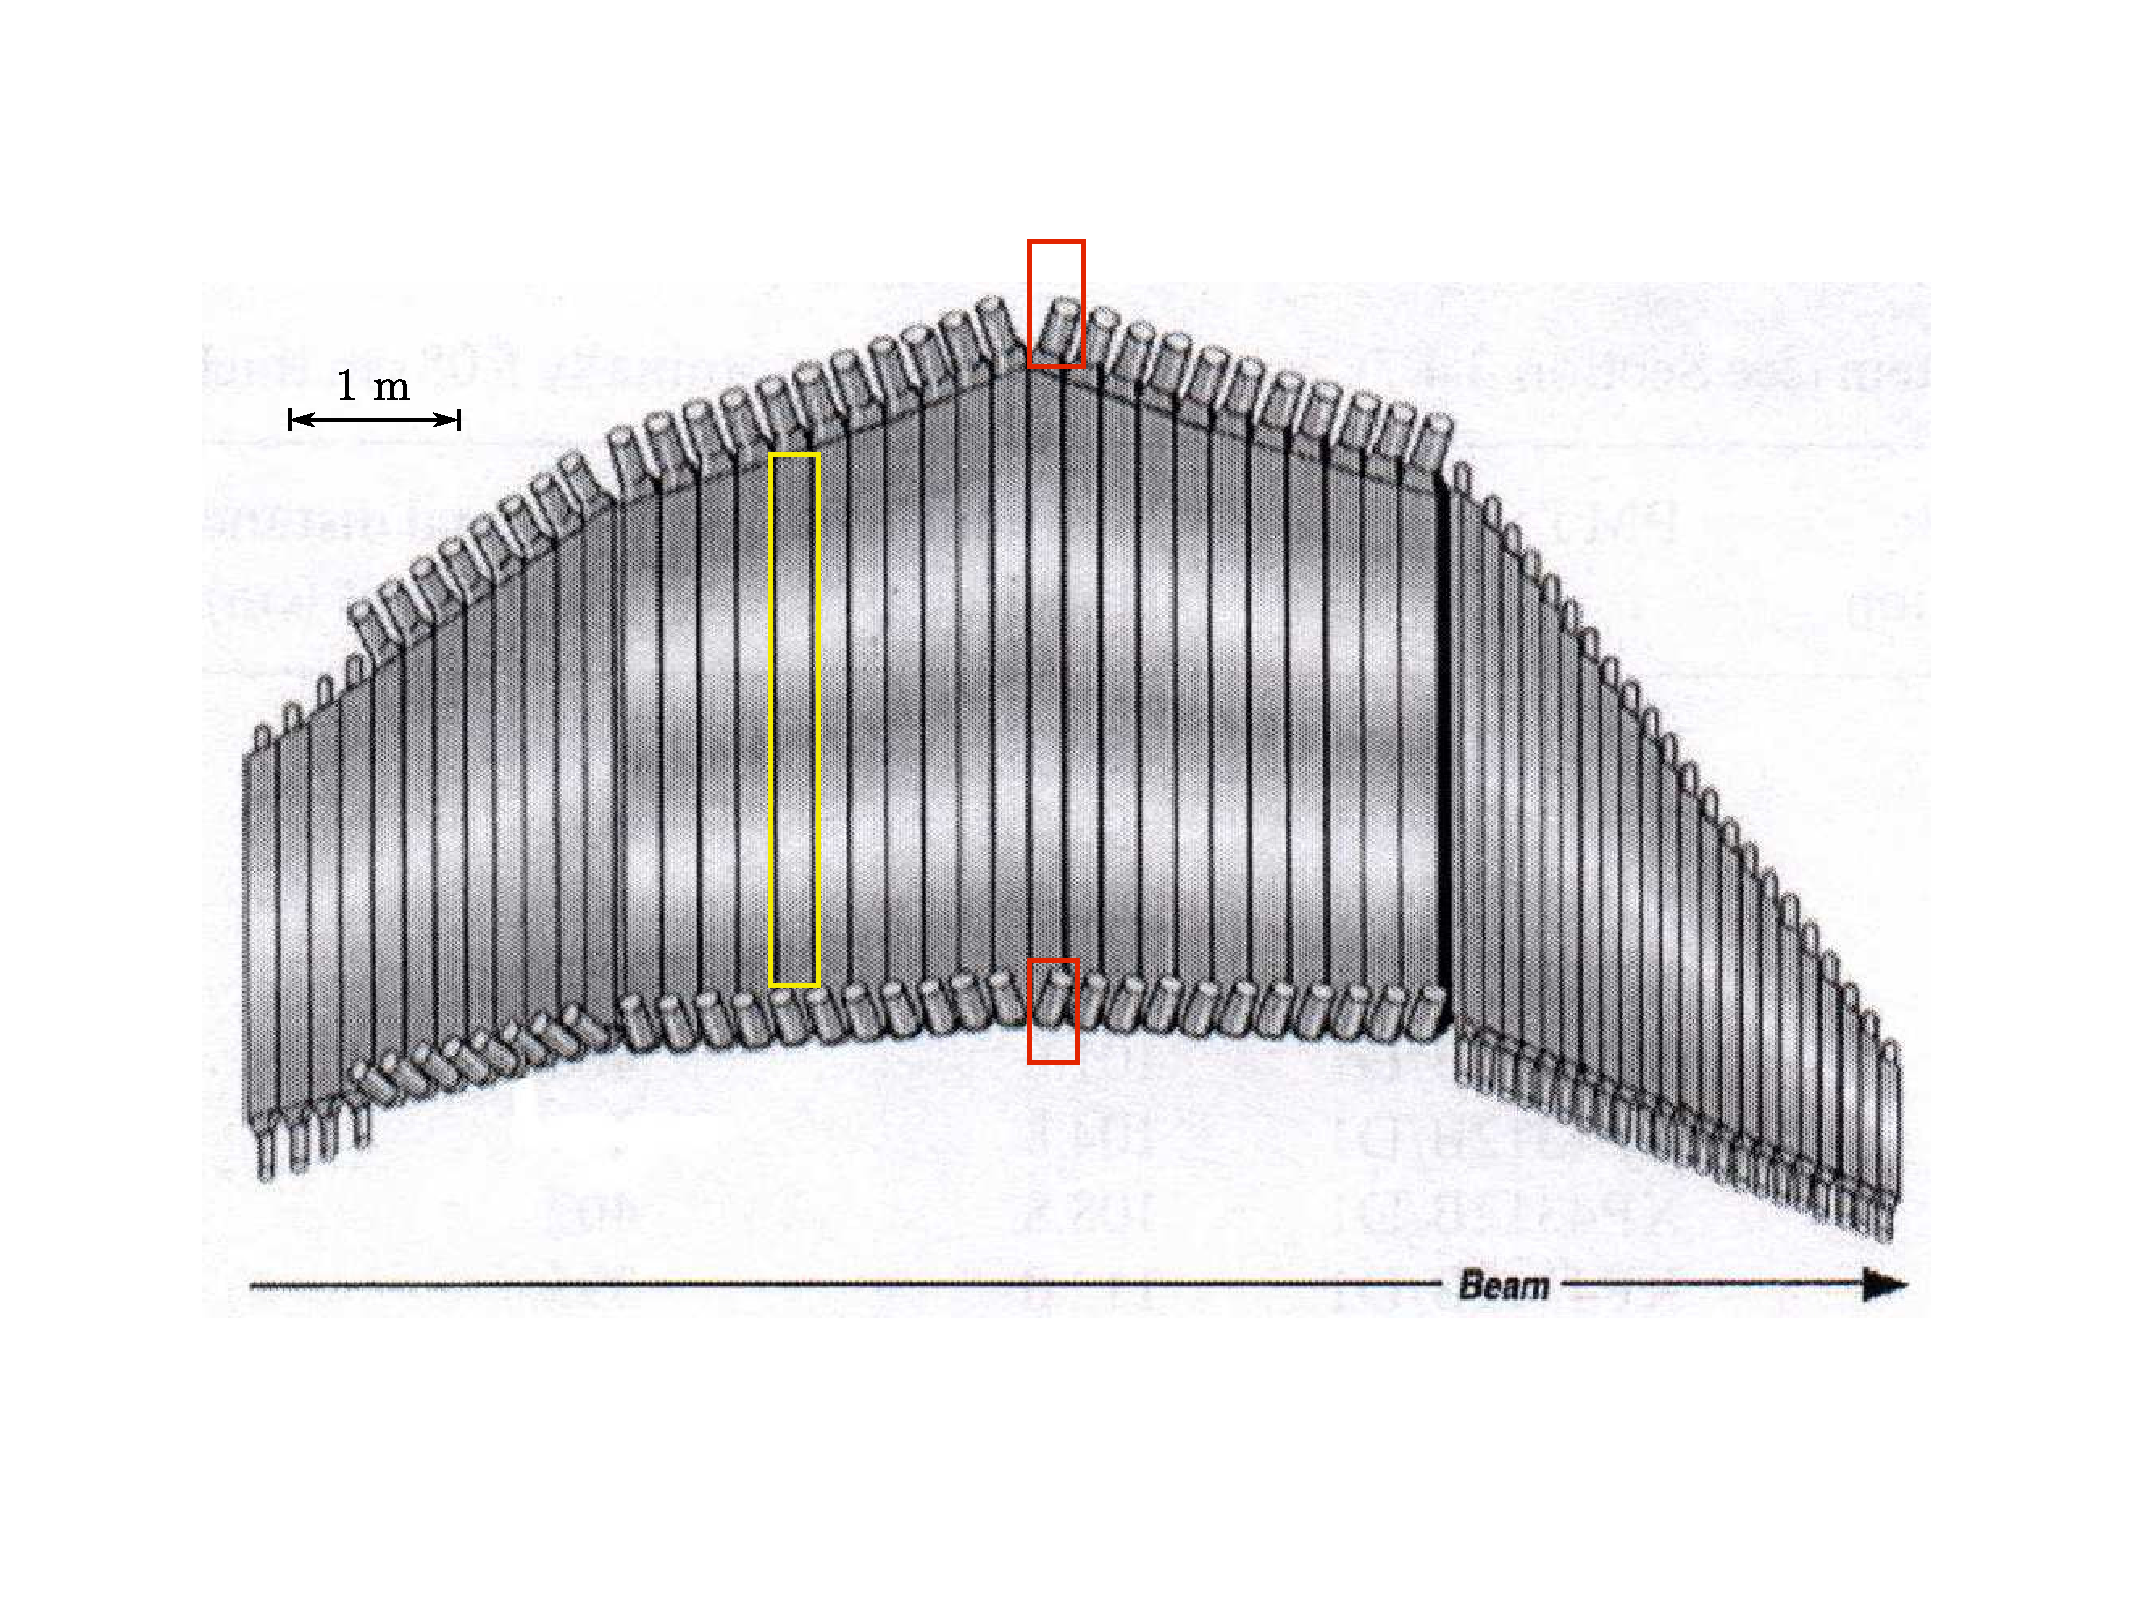
\includegraphics[width=\figwidth]{\figures/hall-b/tof_paddlesII.pdf}
\caption[Diagram of one sector of the time-of-flight (\abbr{TOF}) paddles]{\label{fig:clas.tof.paddles}Diagram of one sector of the time-of-flight (\abbr{TOF}) paddles. There are 57 scintillator paddles covering the entire acceptance region of the drift-chambers for each sector. \abbr{PMT}'s are outlined in red while a scintillator paddle is outlined in yellow.  Image Source:~\cite{clas.tof}}
\end{center}\end{figure}

\FloatBarrier
%\begin{figure}\begin{center}
%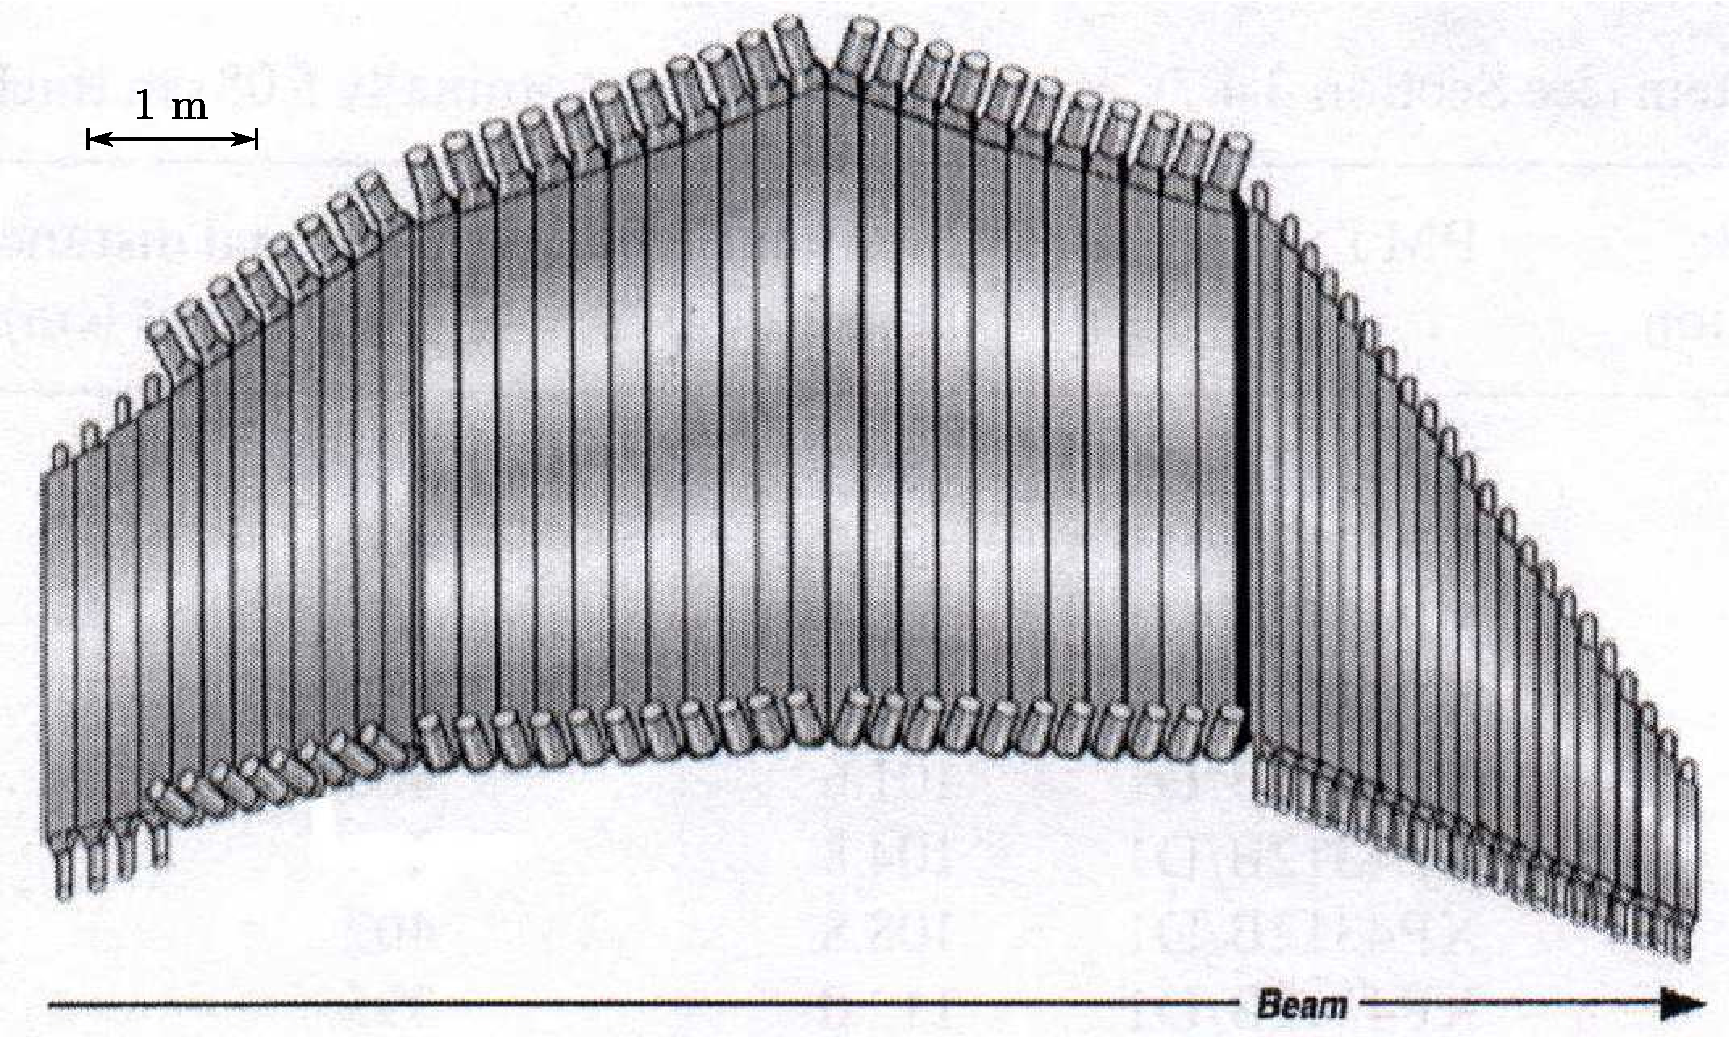
\includegraphics[width=\figwidth]{\figures/hall-b/tof_paddles.pdf}
%\caption[Time-of-Flight Paddles]{\label{fig:clas.tof.paddles}Diagram of one sector of the time-of-flight (\abbr{TOF}) paddles. There are 57 scintillator paddles covering the entire acceptance region of the drift-chambers for each sector.}
%\end{center}\end{figure}
%
%\begin{figure}\begin{center}
%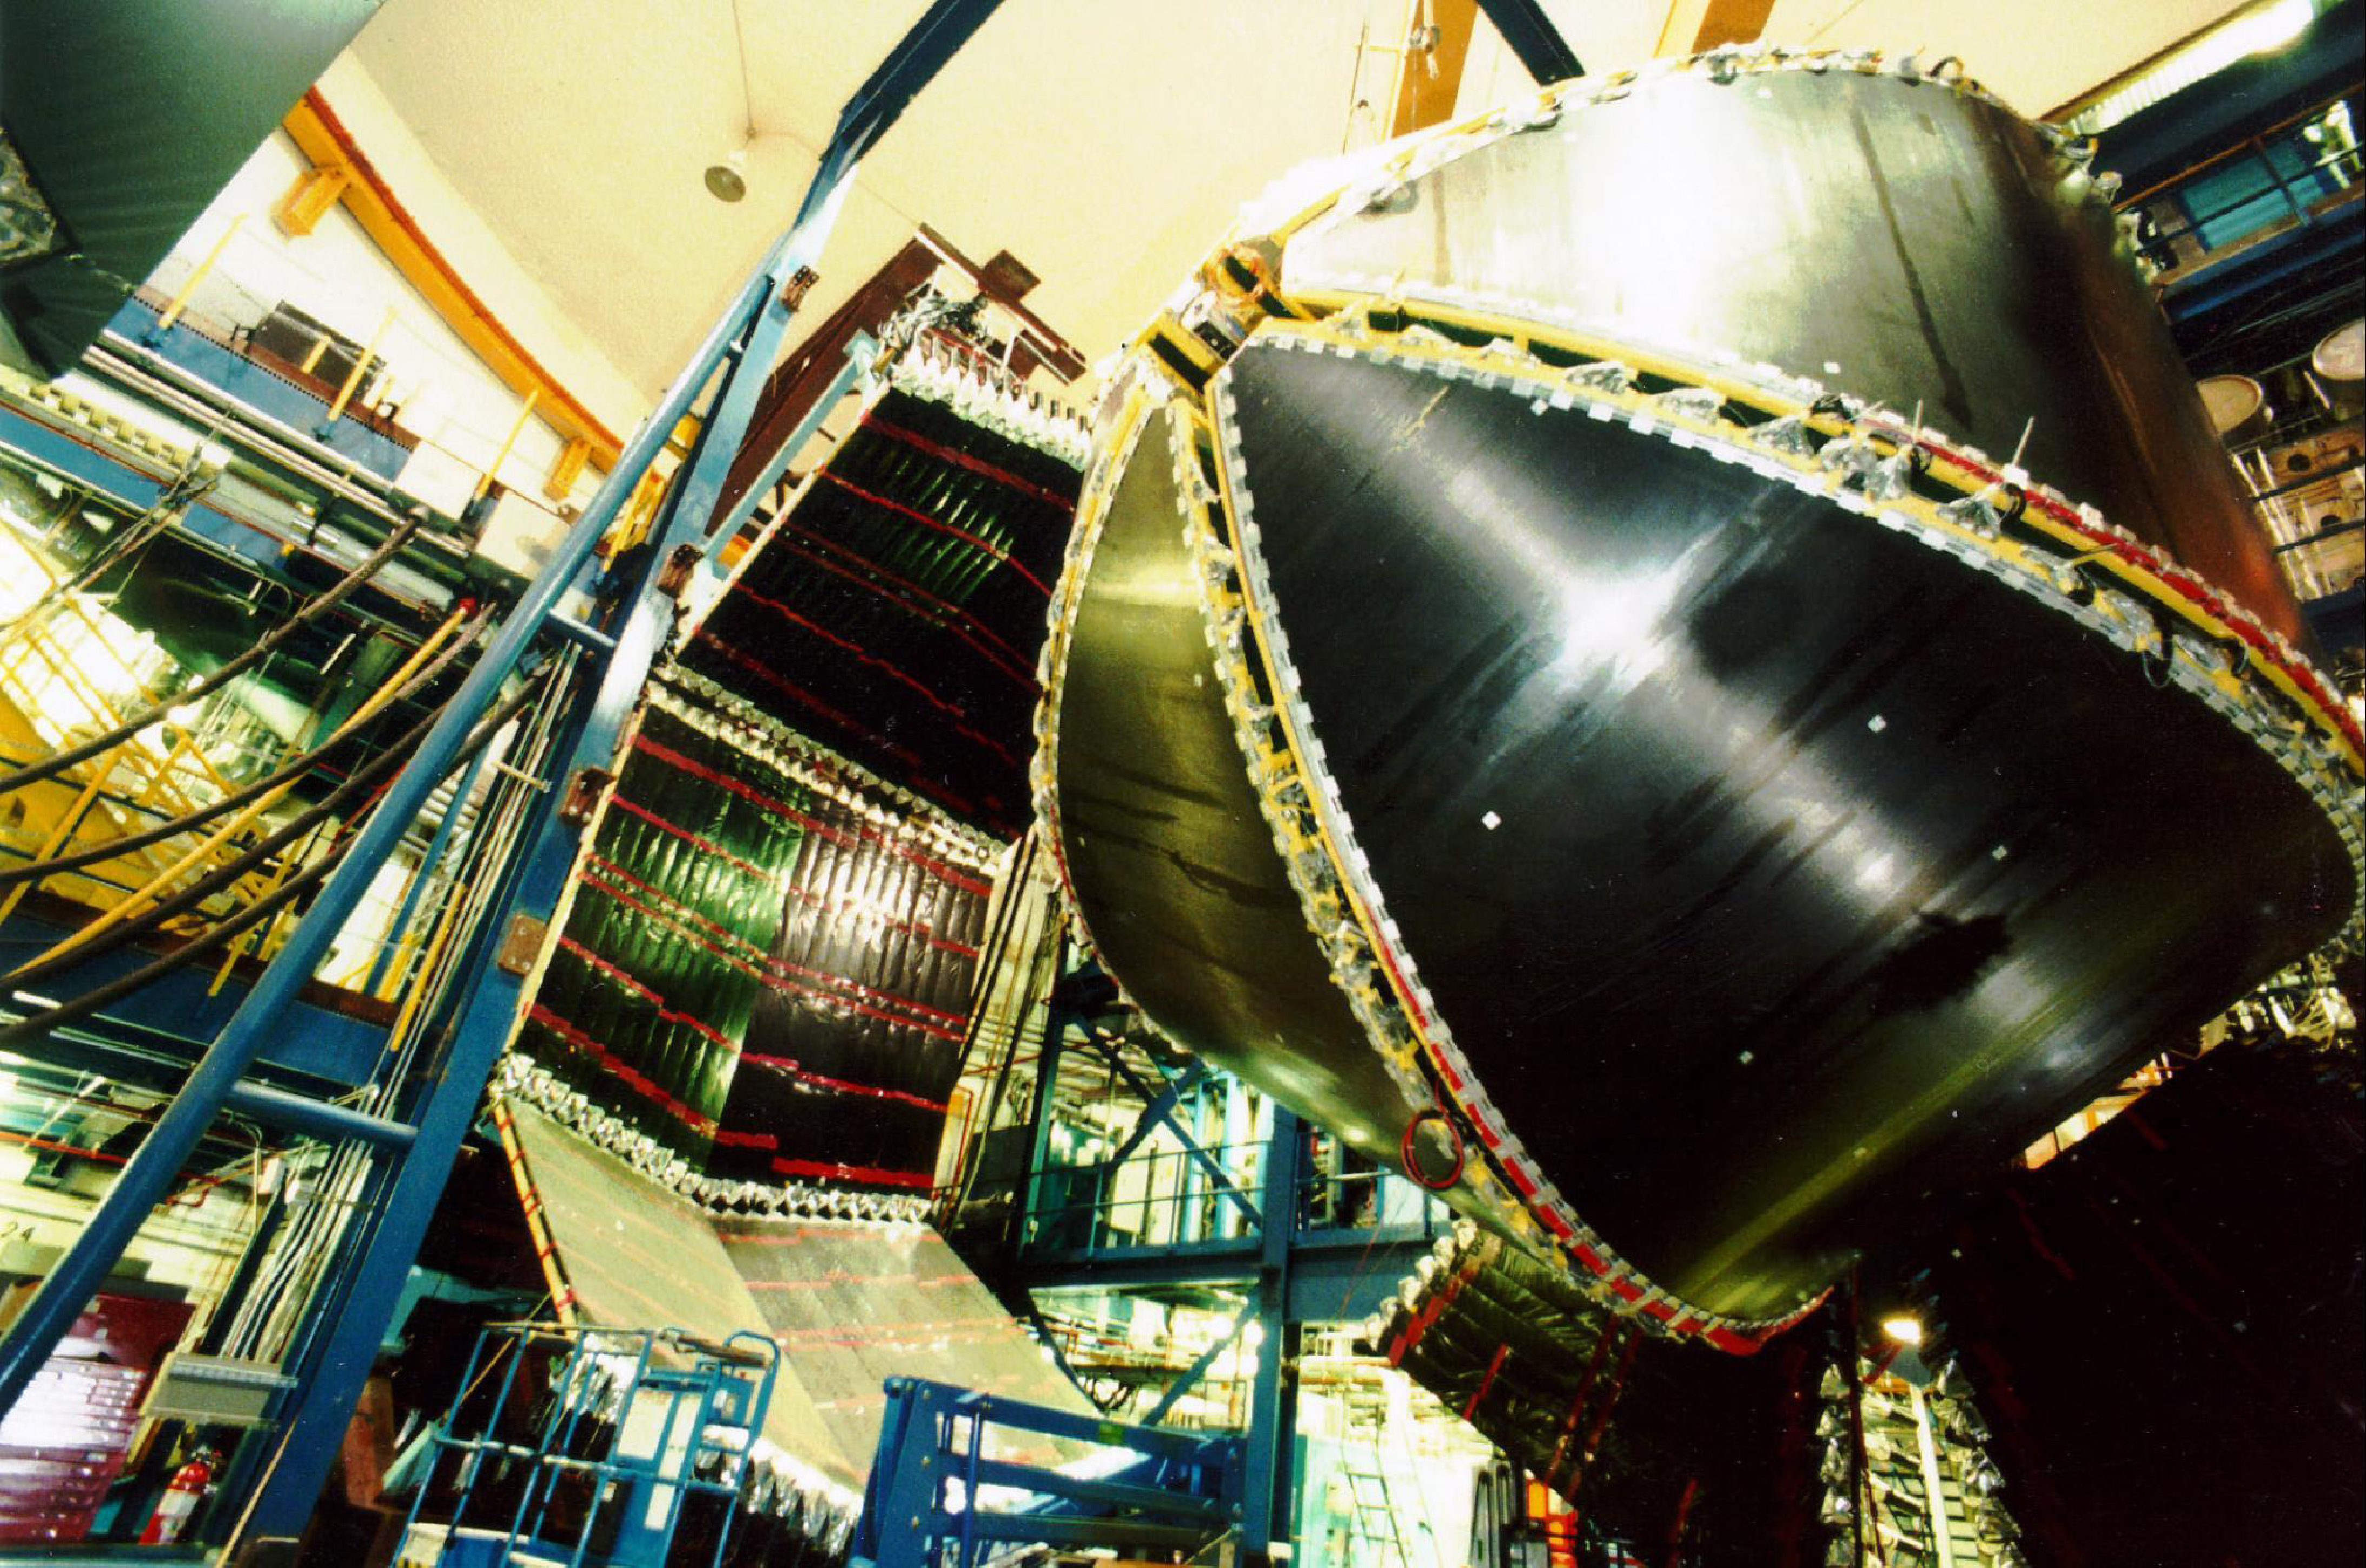
\includegraphics[width=0.8\columnwidth]{\figures/hall-b/clas_detector.pdf}
%\caption[\abbr{CLAS} Detector (photograph)]{\label{fig:clas.photo}The \abbr{CLAS} detector during a maintenance period where the time-of-flight ``shell'' (left) was pulled back from the drift-chambers (\abbr{DC}, right). The beam line enters from the lower right on the other side of the \abbr{DC}. The \abbr{TOF} paddles seen are the two center \emph{panels} shown in Fig.~\ref{fig:clas.tof.paddles} for three of the \abbr{CLAS} sectors.}
%\end{center}\end{figure}
%
%\begin{figure}\begin{center}
%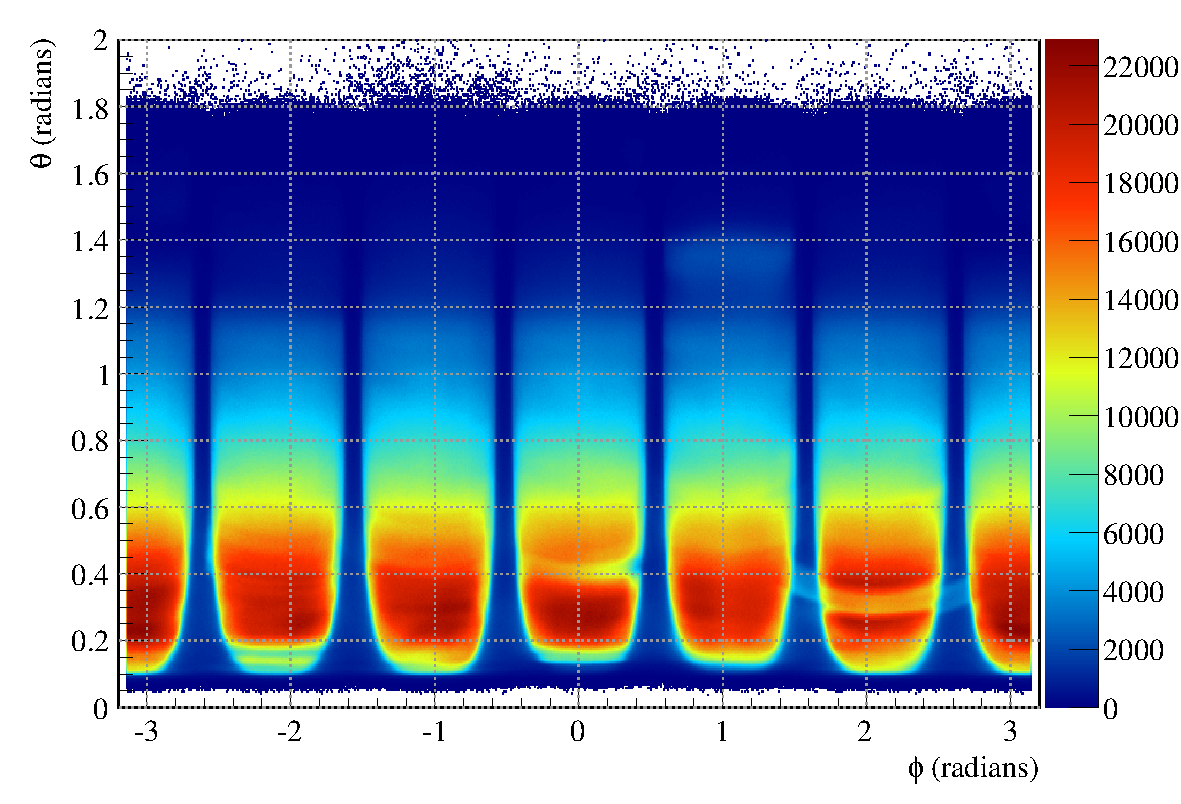
\includegraphics[width=\figwidth]{\figures/reconstruction/coverage_tof.pdf}
%\caption[Time-of-Flight Angular Coverage]{\label{fig:clas.tof.coverage}{\coloronline}Angular coverage in the lab frame of the tracks that had an associated time-of-flight hit. This can be interpreted as the total drift-chamber coverage of the \abbr{CLAS} detector.}
%\end{center}\end{figure}

\FloatBarrier
\section{Cherenkov Radiation and Detectors}\label{sec:clas.cc}

When a charged particle traverses through a medium with a velocity less than the speed of light for that medium ($v < c/n$) the dipoles of the molecules in the medium are symmetrically arranged such that the integrated dipole field along the particles path vanishes. However, when the particles speed is greater than that of the speed of light for that medium the dipoles of the molecules arrange themselves such that they are asymmetric along the particles path and thus creates a dipole field, see Fig~\ref{fig:clas.cc.dipole}.
\begin{figure}[h!]\begin{center}
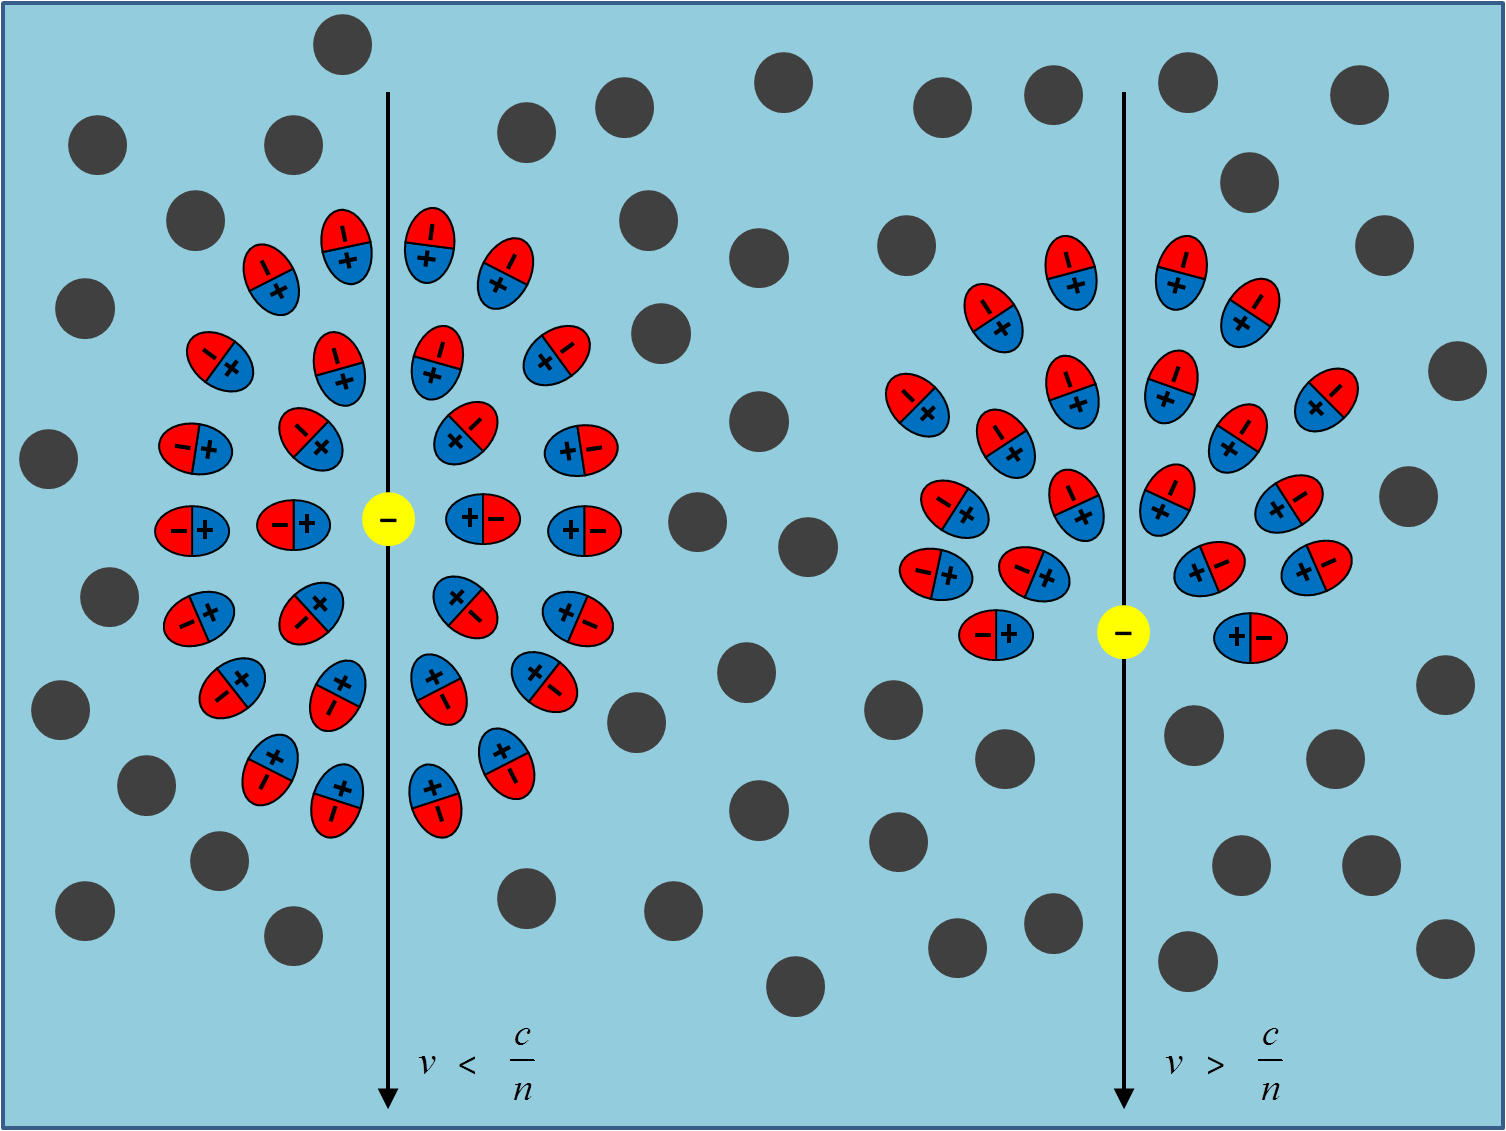
\includegraphics[width=\figwidth,height=\qfigheight]{\figures/hall-b/CCECPLOTS/cherenkov.pdf}
\caption[Illustration of Cherenkov Radiation]{\label{fig:clas.cc.dipole}Illustration of Cherenkov Radiation. Negative charged particle traveling through a medium with $v < c/n$ showing dipoles symmetrically arranged around particles path (left). Negative charged particle traveling through a medium with $v > c/n$ showing dipoles asymmetrically arranged around particles path given rise to dipole field(right). Image Source:~\cite{cherenkov_image}}
\end{center}\end{figure}

The generated dipole field radiates the energy contained in this disturbance producing a coherent shockwave, this is known as Cherenkov radiation. An analogy of this phenomena is the sonic boom created in air from an object traveling faster then the speed of sound. Just as the sound wave of a sonic boom travels slower than the traveling object, so does the light emitted from the dipole field. This reduction in velocity creates the wave front of a continuous light spectrum, see Fig~\ref{fig:clas.cc.angle}.
\begin{figure}[h!]\begin{center}
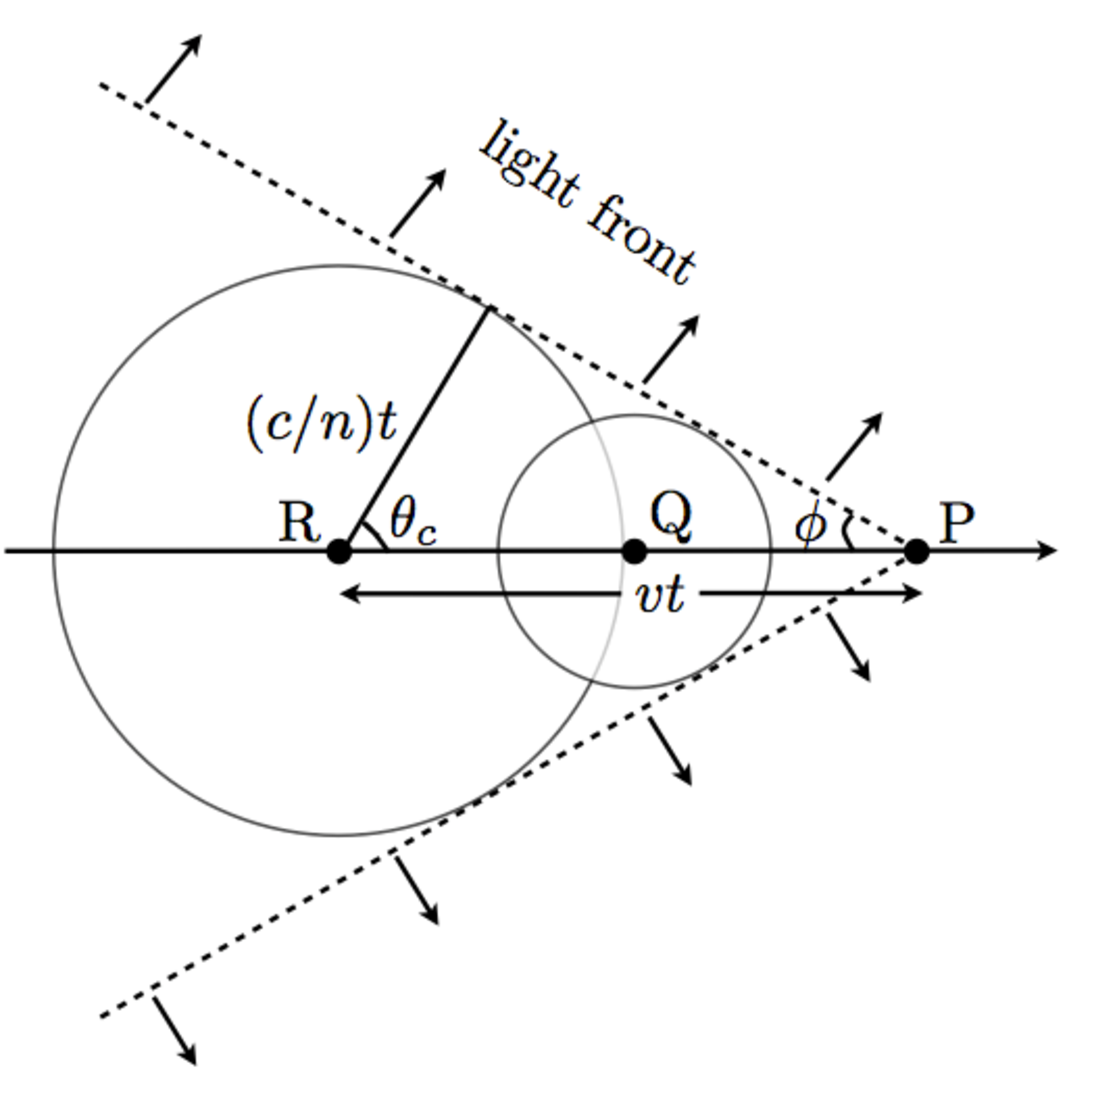
\includegraphics[width=\figwidth,height=0.75\hfigheight]{\figures/hall-b/CCECPLOTS/cc_wavefront_madeII.pdf}
\caption[Illustration of Cherenkov Angle]{\label{fig:clas.cc.angle}Illustration of Cherenkov Angle. When the particle has traveled the distance $\mathrm{RP =\nu t \rightarrow \beta c t}$, the photon (light front) has traveled $(c/n)t$.}
\end{center}\end{figure}

Inspecting Fig~\ref{fig:clas.cc.angle}, when the particle has traveled the distance $\mathrm{RP =\nu t = t \beta c}$, the photon has traveled $(c/n)t$, therefore
\begin{equation}\label{eq:cherenkov_eq}
 \mathrm{\cos\theta_{c} = \frac{(c/n)t}{t \beta c} = \frac{1}{n\beta}}
\end{equation}
and the threshold of Cherenkov radiation is 
\begin{equation}\label{eq:cherenkov_threshold}
 \mathrm{\beta_{th} > \frac{1}{n}}.
\end{equation}
Adding in quantum effects
\begin{equation}\label{eq:cherenkov_eq_quantum}
\mathrm{cos\theta_{c} = \frac{1}{n\beta} + \frac{\Lambda}{\lambda}\frac{n^{2} -1}{2n^{2}}}
\end{equation}
where
\begin{equation}\label{eq:cherenkov_eq_quantum_lambda}
\mathrm{\Lambda = \frac{\sqrt{1-\beta^{2}}}{\beta}\lambda_{0}} \ , 
\end{equation}
$\mathrm{\lambda =}$ wavelength of light in medium, and $\mathrm{\lambda_{0} }$ is the Compton wavelength 0.024 \AA. For practical cases, and using \abbr{CLAS}, the 2$^{nd}$ order term is negligible (n=1.00153). To illustrate that quantum effects are negligible, an electron traveling at threshold in \abbr{CLAS} \abbr{CC},
\begin{equation}
\mathrm{\beta_{th} > \frac{1}{n}} > 0.998472,
\end{equation}

\begin{equation}
\mathrm{\frac{\Lambda}{\lambda}\frac{n^{2} -1}{2n^{2}} =  1.07874 \cdot 10^{-9}}
\end{equation}
%

In \abbr{CLAS}, the Cherenkov counter (\abbr{CC}) is used to detect electrons and positrons while rejecting pions for momenta less than 2.5~GeV. The gas used in the \abbr{CC} for \g12 is perfluorobutane (C$_4$F$_{10}$) with an index of refraction of 1.00153. The threshold energy for producing Cherenkov radiation in C$_4$F$_{10}$ is
\begin{align}
\mathrm{E_{th} = \gamma_{th} m_{0}} \mathrm{ \ (Units \ of \ c)} \\
\mathrm{\gamma_{th} = \frac{n}{\sqrt{n^{2} -1}}} = 18.09
\end{align}
therefore the threshold energy of e$^{\pm}$ is 9.23~MeV while the threshold energy of $\pi^{\pm}$ is 2.52~GeV.
%
The number of photons emitted per unit length at threshold for electrons or positrons is;
\begin{align}\label{eq:cc.NPE}
\frac{dN}{dx} = 2\pi z^2 \alpha \frac{\sin \theta_{c}^2}{\lambda^2} d\lambda = 0.241246 \frac{d\lambda}{\lambda^2}
\end{align}
where $\alpha$ is the fine structure constant, $z =1$ for electrons and positrons, and $\lambda$ is the wavelength at which the photon is emitted. Table~\ref{tab:cc_npe} lists the number of photons/cm for various wavelengths of light for the midpoint of $\beta_{th}$ and a maximum velocity $\beta =1$. Table~\ref{tab:cc_npe} also lists the mirror reflectivity for that wavelength.
\begin{table}[h!]
\begin{minipage}{\textwidth}
\begin{center}
\begin{singlespacing}

\caption[Number of Photo-electrons per Unit Length in Cherenkov Detection]{\label{tab:cc_npe}Number of $\gamma$'s per unit length gas $C_4F_10$ \vspace{0.75mm}}

\begin{tabular}{c|c|c|c}

\hline
Wavelength~nm & \multicolumn{2}{c|}{$\frac{dN}{dx}$~photons/cm} & Mirror reflectivity~\cite{clas.cc}  \vspace{0.5mm} \\
\hline
&$\beta = \frac{1}{2}(1+\beta_{th})$& $\beta = 1$ \\
\hline
400-700 (visible) & $0.75$ & $1.5$ & 90\% \\
300-400 (near UV) & $0.6$ & $1.2$ & 85 - 90 \% \\
190-300 (near UV) & $1.4$ & $2.7$ & 20 - 85\% \\
\hline \hline
\end{tabular}
\end{singlespacing}
\end{center}
\end{minipage}
\end{table}
\vspace{20pt}


The \abbr{CC} subsystem is physically located in the space between Region 3 of the \abbr{DC} subsystem and the \abbr{TOF} in the forward region covering polar angles 8$^\circ$ to 45$^\circ$ in each sector when the target is at \abbr{CLAS} center. For \g12 since the target was placed 90~cm upstream, the polar coverage was approximately from 6$^\circ$ to 35$^\circ$ in the lab frame. The \abbr{CLAS} \abbr{CC}'s were fabricated as 6 independent identical sectors, with each sector divided into 18 regions of $\mathrm{\theta}$, and each $\mathrm{\theta}$ segment divided into 2 modules. Light from Cherenkov radiation is focused in $\mathrm{\phi}$ thus preserving information on the lepton polar angle $\theta$. The optical element of \abbr{CC} module comprises an assembly of one elliptical and one hyperbolic mirror providing primary light focusing into a  ``Winston" light collection cone, a  cylindrical mirror used to compensate for imperfections in the focusing, and a photomultiplier used to count the  number of photons in the light cone, see Fig~\ref{fig:clas.cc_array}. More information on the \abbr{CLAS} Cherenkov detector can be found in~\cite{clas.cc} 

The use of the \abbr{CC} was not included in the original proposals, however a significant drop in price on C$_4$F$_{10}$ just prior to the start of \g12 allowed the gas to be added at the last minute. The price drop was due to the recent availability of another, much cheaper gas that was demonstrated to have the same general properties as C$_4$F$_{10}$ and when \g12 contacted the original supplier of the C$_4$F$_{10}$ for a price match, they committed. 

\begin{figure}[h!]\begin{center}
\subfloat[]{
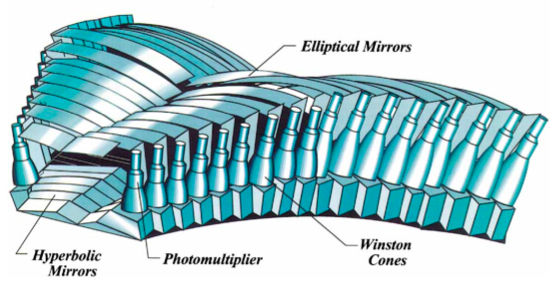
\includegraphics[width=\figwidth,height=0.5\hfigheight]{\figures/hall-b/CCECPLOTS/CCarray}\label{fig:clas.cc_array}
}\\
%[Schematic of one \abbr{CC} showing the 18 symmetrical, mirrored segments of the CLAS \abbr{CC}]
\subfloat[]{
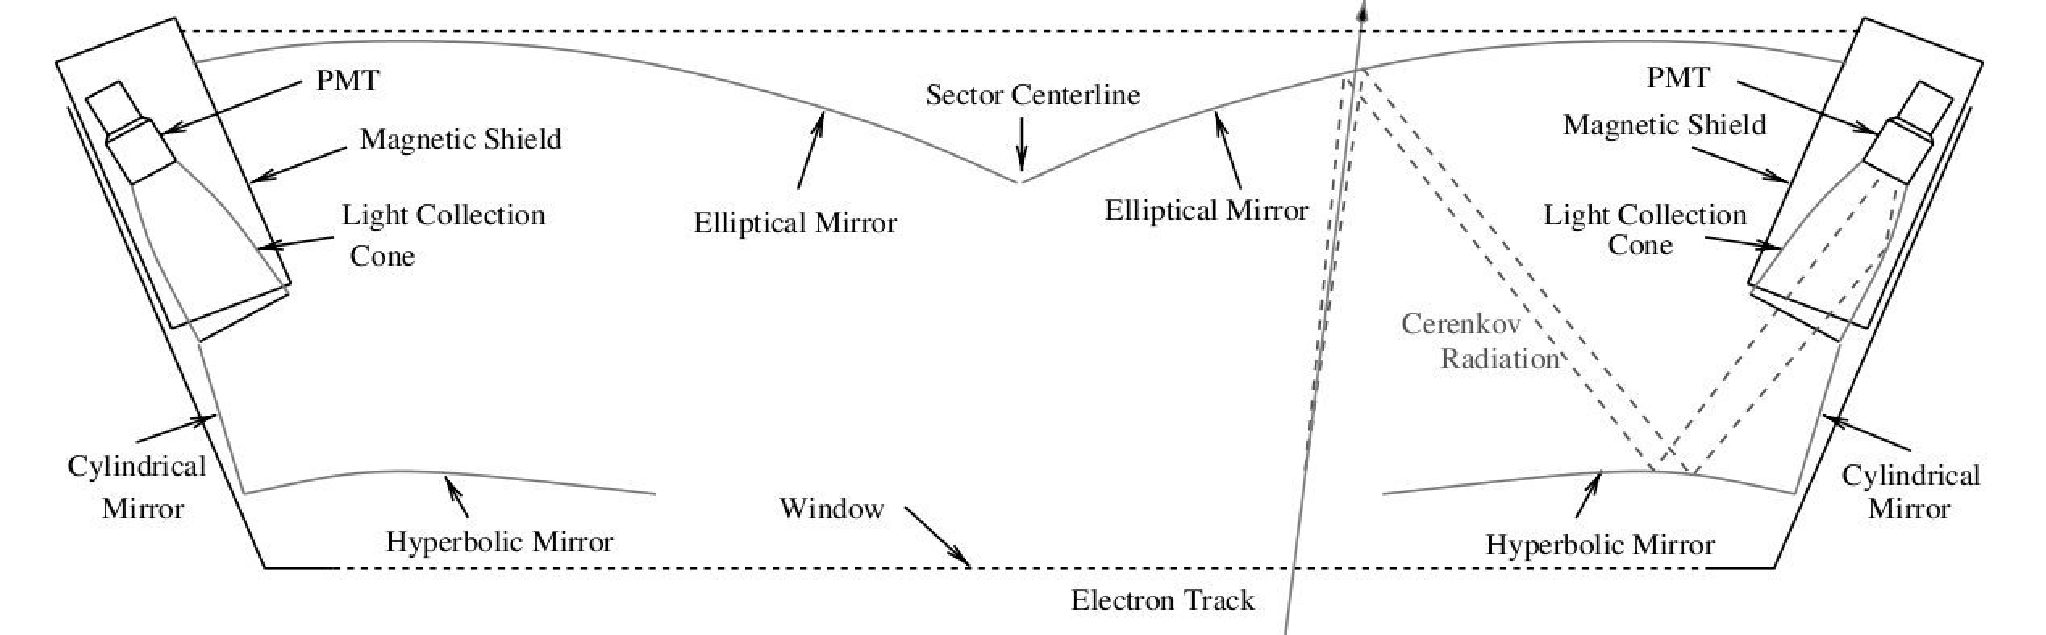
\includegraphics[width=0.9\columnwidth]{\figures/hall-b/cc_diagram.pdf}\label{fig:clas.cc}
}
\caption[Schematic of one \abbr{CC} showing the 18 symmetrical, mirrored segments of the CLAS \abbr{CC}]{Schematic of one \abbr{CC} showing the 18 symmetrical, mirrored segments of the CLAS \abbr{CC}~(a). Diagram of one segment of the Cherenkov counters with an electron entering from the bottom~(b).}

\end{center}\end{figure}






\section{Electromagnetic Calorimeters}\label{sec:clas.ec}

The calorimetric method implies total absorption of the particle energy in a bulk of material followed by the measurement of the deposited energy. The process usually involves several layers of absorbers and detectors. Depending on the energies and species of particles there are different types of calorimeters. For instance, a 10~GeV muon will require 9~m of Fe or 8~m of Pb to absorb all the energy of the muon. However, a 10~GeV electron will only require 0.2~m of Pb to absorb all the energy.The Electromagnetic Calorimeter was built and used for detection of neutral particles as well as discrimination between electrons and pions.

%\begin{figure}[h!]\begin{center}
%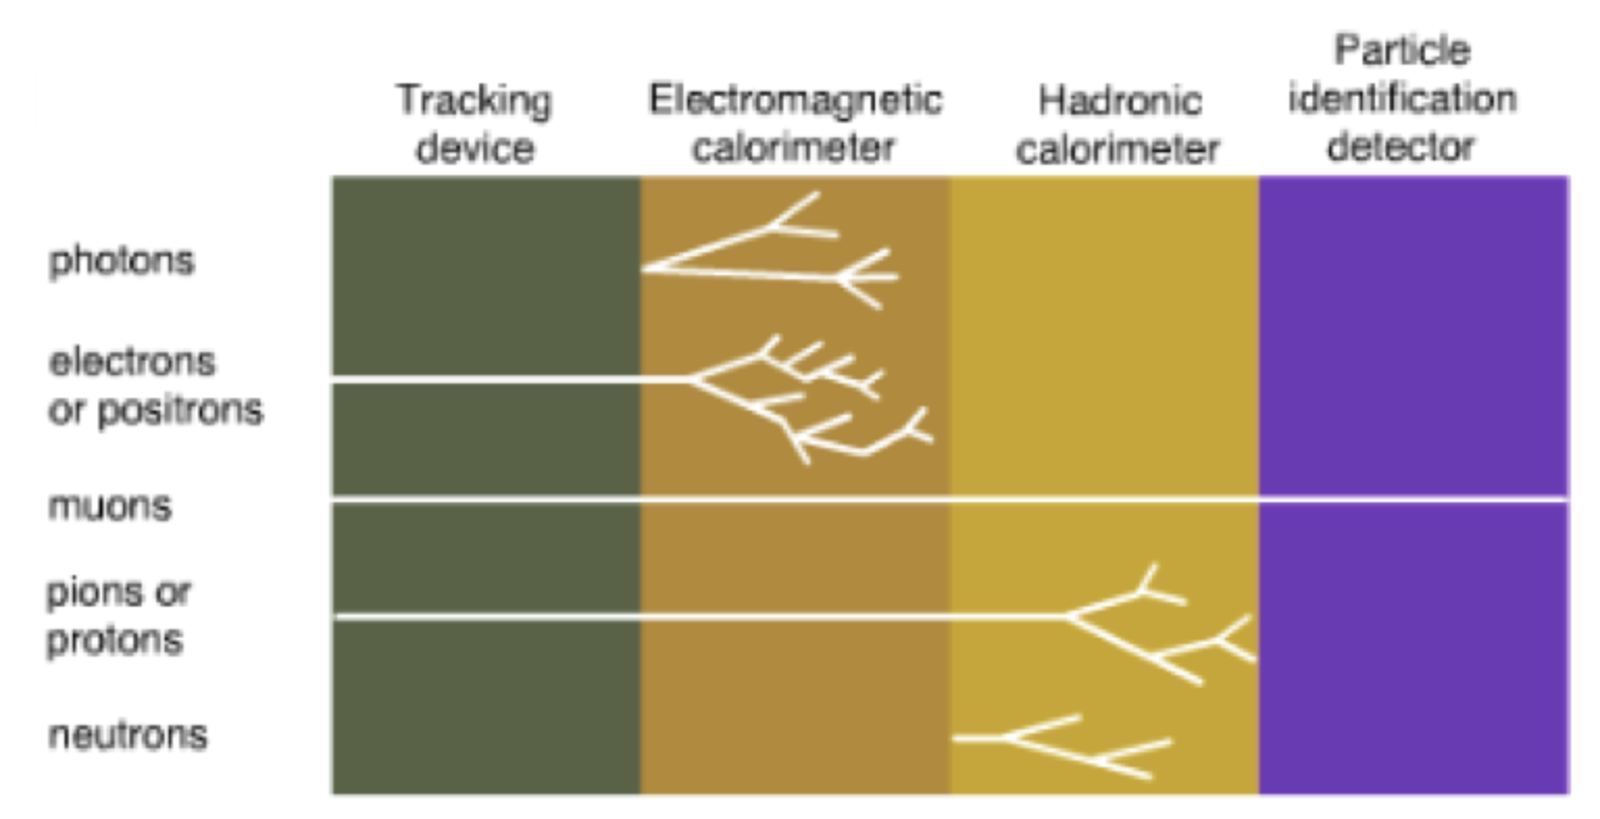
\includegraphics[width=\figwidth,height=\qfigheight]{\figures/hall-b/CCECPLOTS/Calorimetry/detectors.pdf}
%\caption[Types of Calorimeters]{\label{fig:clas.ec.calorim}Type of calorimeter depends on type of hadron detection Image Source:~\cite{C5}}
%\end{center}\end{figure}

\subsection{Electromagnetic Calorimeter}

At energies greater than 100~MeV, electrons lose their energy predominantly by bremsstrahlung while photons lose their energy by electron-positron pair production. The process of bremsstrahlung is electromagnetic radiation produced by the deceleration of an electron when deflected by an atomic nucleus i.e. $\mathrm{e Z \rightarrow Ze\gamma}$. Its cross-section is proportional to $\mathrm{Z^{2}}$ of the material the electron propagates through. The radiation loss of electrons with initial energy $E_0$ can be described as
\begin{align}\label{eq:electron_eloss}
-(\frac{dE}{dx})_{rad} = \frac{E}{X_{0}} \\ \vspace*{10 mm} E(x)=E_{0}e^{\frac{-x}{X_{0}}} 
\end{align}
where $X_{0}$ is the radiation length of the material the electron travels through. The process of pair production, $\gamma Z \rightarrow Ze^{+}e^{-}$ was discussed in Sec.~\ref{sec:intro.conversion}.
%, occurs when a photon with $E_0 > 2 m_e c^2$ converts into an electron and a positron. The cross section for this process can be simplified as
%\begin{equation}\label{pair_crosssection}
%\sigma_{\gamma\rightarrow e^+e^-} =  \frac{A}{N_{A} \rho \lambda_\gamma}  \ ,\ \lambda_\gamma = \frac{9}{7}X_0
%\end{equation}
%where $\lambda$ is also know as the interaction length, or mean free path, $\rho$ is the density of the material, $N_A$ is Avogadro's number and $A$ being the atomic mass of the material. The probability of pair production to occur is solely based on $X_{0}$, the radiation length of the medium and this probability can be expressed as
%\begin{equation}
%\frac{dP}{dx} = \frac{1}{\lambda_\gamma}\exp(\frac{-x}{\lambda_\gamma}) \ .
%\end{equation}

To explain how an Electromagnetic Calorimeter works, assume the absorber for the calorimeter is lead(Pb), Fig \ref{fig:clas.photon_processes} , \ref{fig:clas.electron_processes} depicts the processes for photons and electrons in Pb.
\begin{figure}[h!]\begin{center}
\subfloat[][]{
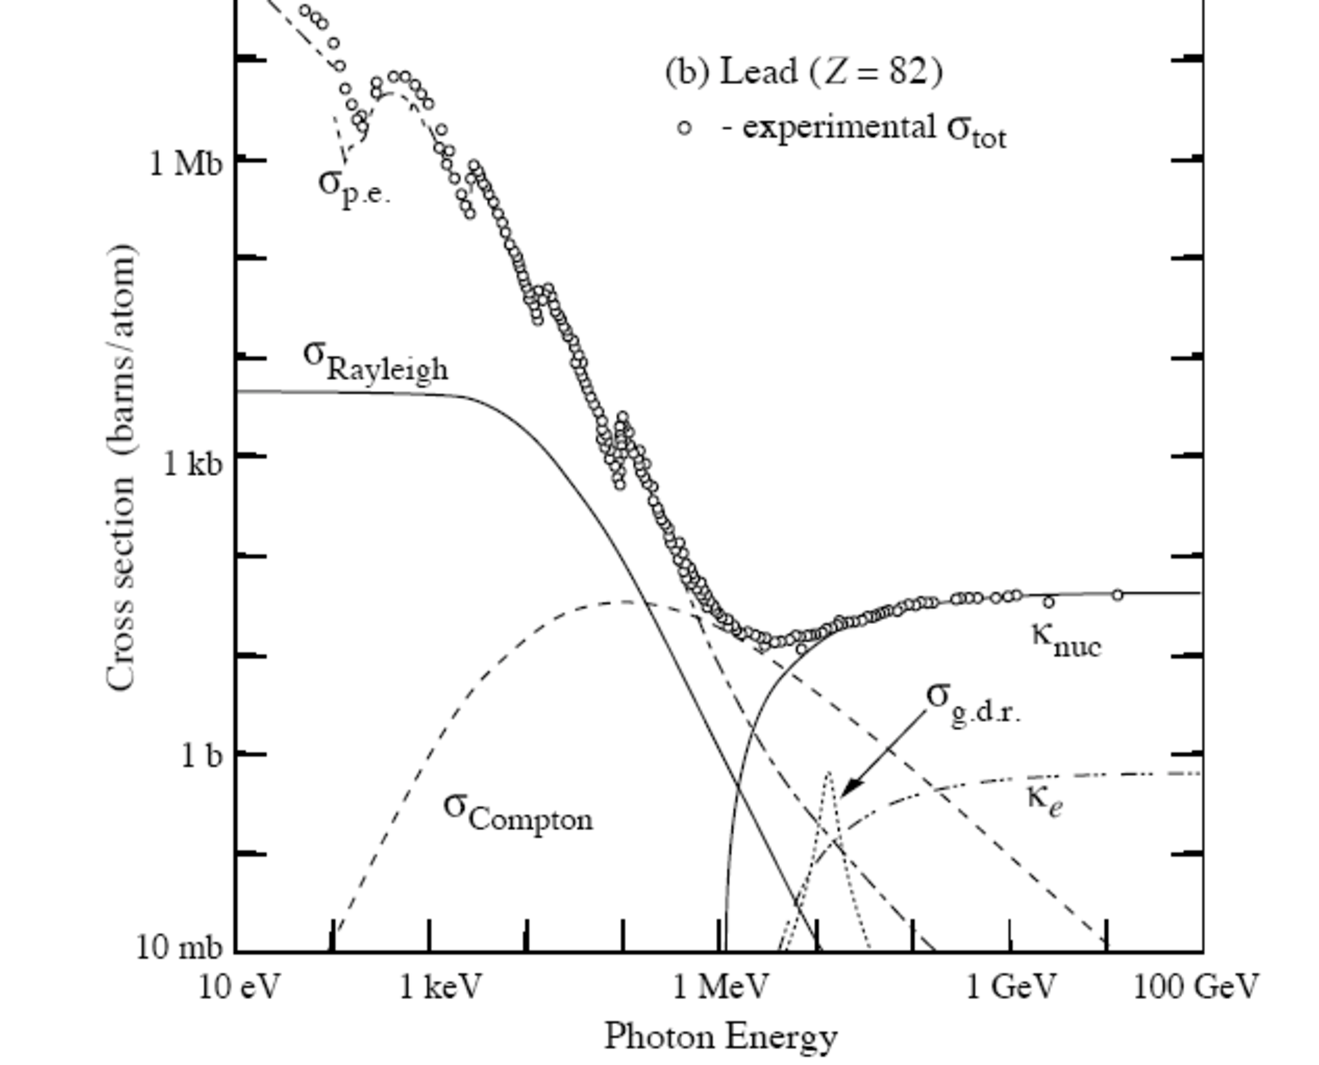
\includegraphics[width=0.45\columnwidth,height=0.5\hfigheight]{\figures/hall-b/CCECPLOTS/Calorimetry/PhotonRadiations.pdf}\label{fig:clas.photon_processes}
}
\subfloat[][]{
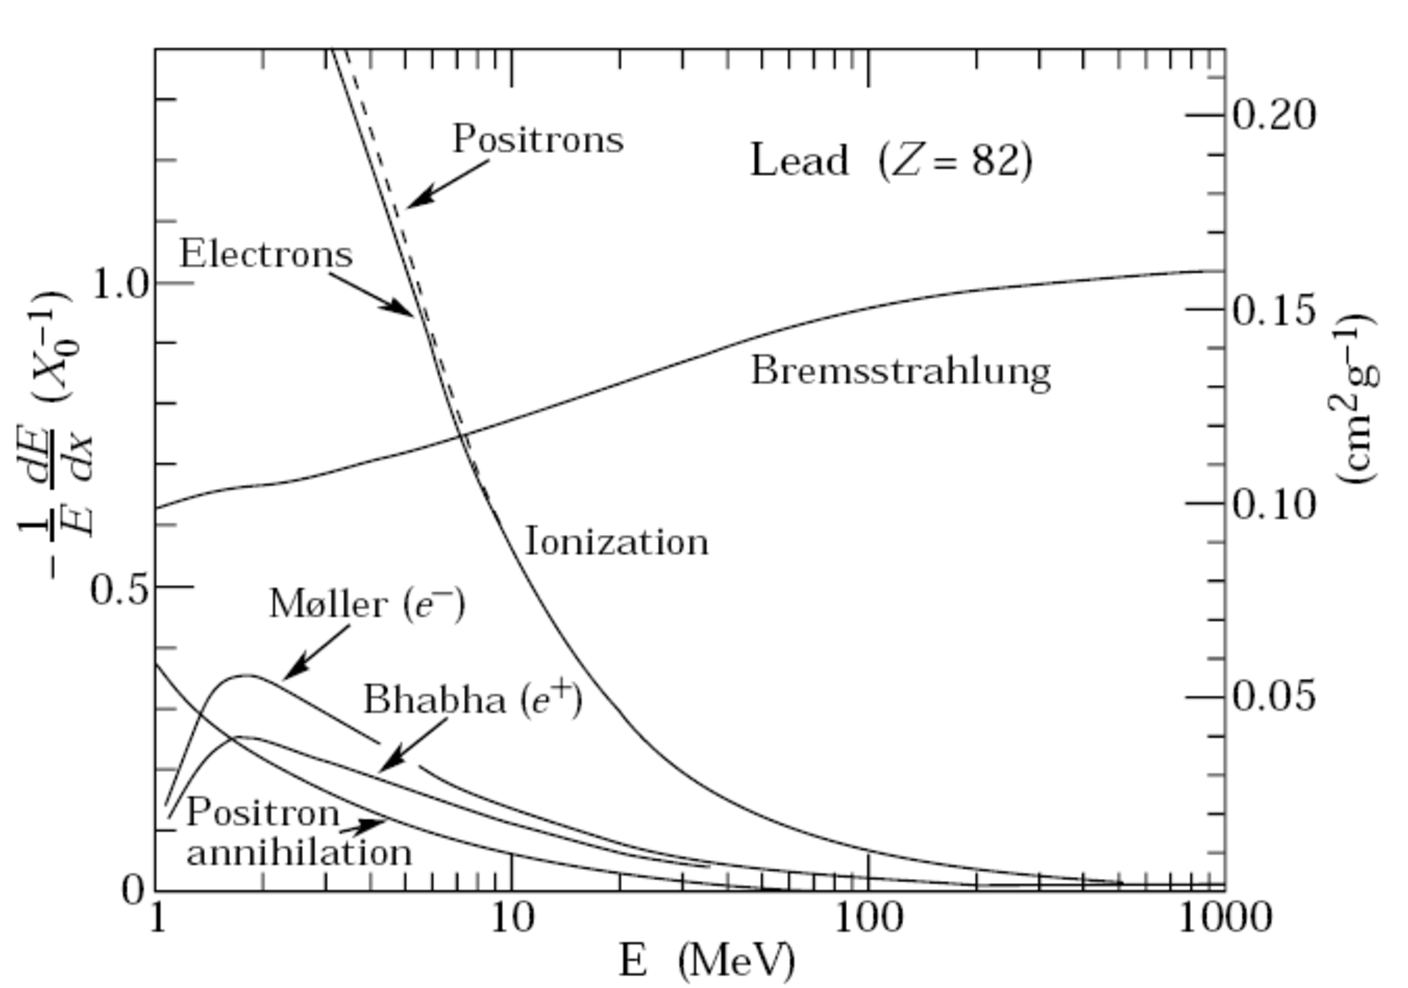
\includegraphics[width=0.45\columnwidth,height=0.5\hfigheight]{\figures/hall-b/CCECPLOTS/Calorimetry/EectronE2.pdf}\label{fig:clas.electron_processes}}
\caption[Photon and Electron processes in \abbr{Pb}]{Photon and Electron processes in \abbr{Pb}~(a) and (b) respectively. Images Source:~\cite{vibe_levels}} 

\end{center}\end{figure}
Lets start with a high energy electron $E_{0}$, after $1 X_{0}$, $\mathrm{1e^{-}}$ and $\mathrm{1 \gamma}$ are produced each with $\frac{E_{0}}{2}$, after $2 X_{0}$, $\mathrm{2e^{-}}$, $\mathrm{1e^{+}}$ and $\mathrm{1 \gamma}$ are produced each with $\frac{E_{0}}{4}$. Therefore after $tX_{0}$, there is a total of 
\begin{equation}
N(t)=2^{t}
\end{equation}
are produced each with
\begin{equation}
E(t) = E_{0}2^{-t}.
\end{equation}
The multiplication of the shower particles continue as long as
\begin{equation}
\frac{E_{0}}{N} > E_{c},
\end{equation}
where $E_{c}$ is the critical energy for showers to propagate,
\begin{align}
E_{c}  = E_{0}2^{-t_{max}} \\
N_{max}=\frac{E_{0}}{E_{c}}
\end{align}

\begin{figure}[h!]\begin{center}
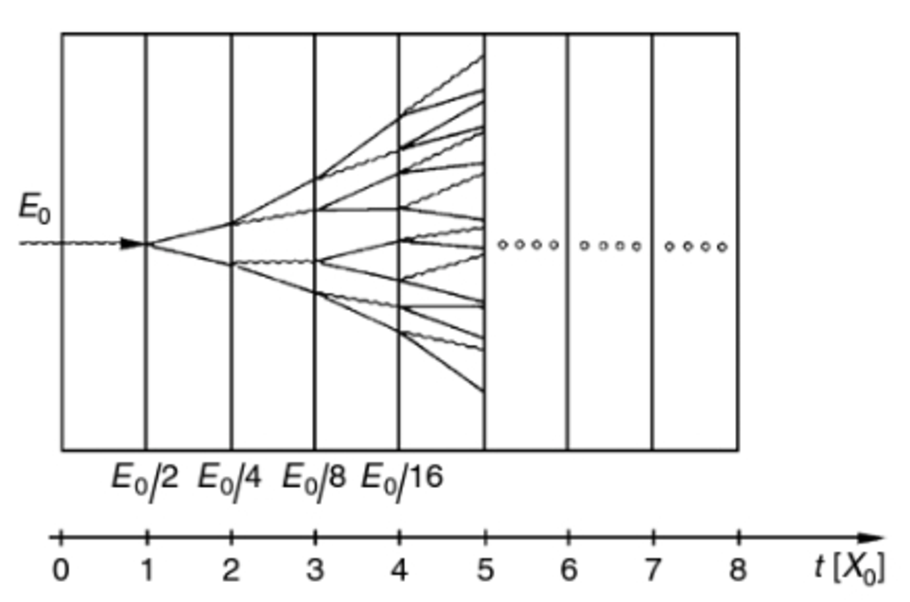
\includegraphics[width=\figwidth,height=\qfigheight]{\figures/hall-b/CCECPLOTS/Calorimetry/cascade.pdf}
\caption[A simple Electromagnetic shower in a calorimeter]{\label{fig:clas.ec.shower}{A simple Electromagnetic shower in a calorimeter} Image Source:~\cite{vibe_levels} }
\end{center}\end{figure}

When a particle falls below critical energy, absorption processes (ionization, Compton and photoelectric) start to dominate the processes for photons and electrons. This leads to
\begin{equation}
t_{max} = \frac{ln(\frac{E_{0}}{E_{c}})}{ln2}.
\end{equation}
At the shower maximum $\mathrm{e^{\pm}}$ will stop within $1X_{0}$ however, photons at critical energy will penetrate further. To absorb 95\% of photons produced in the shower maximum, an additional 7-9$X_{0}$ is necessary. The semi-empirical value for $\mathrm{e^{\pm}}$ $E_c$ in Pb is,
\begin{equation}
E_{c}  \thickapprox \frac{610 MeV}{\mathrm{Z} - 1.24} = 7 MeV 
\end{equation}
which results in $t_{max} \thickapprox 9.7 X_{0}$ for electrons at 6 GeV.

The process shown in Fig~\ref{fig:clas.ec.shower} is a very crude and simple model of an actual shower shown in Fig~\ref{fig:clas.ec.showerII}, but the simple model correctly describes the important features of Electromagnetic Calorimeters
\begin{itemize}
\item The total calorimeter thickness should be more than 10-15~$X_0$ in order to absorb almost all of the energy of an incident photon
\item The position of the shower maximum increases with energy, therefore the thickness of the calorimeter should increase as the logarithm of the energy.
\item If there is energy leakage, it is caused by photons escaping the calorimeter at the sides or at the back.
\end{itemize}

 
\begin{figure}[h!]\begin{center}
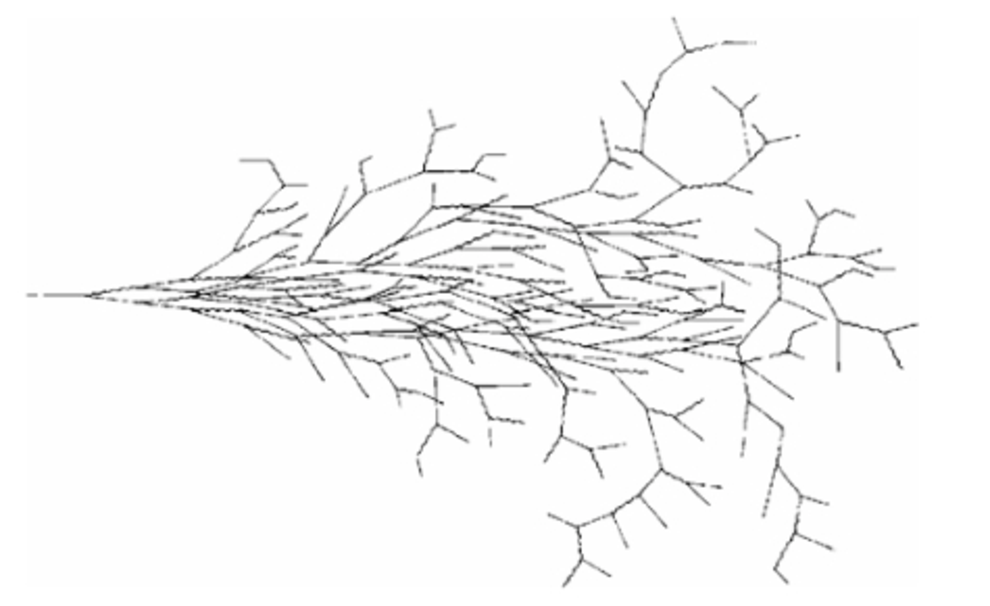
\includegraphics[width=\figwidth,height=\qfigheight]{\figures/hall-b/CCECPLOTS/Calorimetry/cascadeII.pdf}
\caption[A real Electromagnetic shower in a calorimeter]{\label{fig:clas.ec.showerII}{A real Electromagnetic shower in a calorimeter} Image Source:~\cite{vibe_levels} }
\end{center}\end{figure}

\subsection{The \abbr{CLAS} Electromagnetic Calorimeter}

The \abbr{CLAS} electromagnetic calorimeter (\abbr{EC})\cite{clas.ec}, shown in Fig.~\ref{fig:clas} was designed with the following criteria;
\begin{itemize}
\item $\mathrm{e/ \gamma}$ energy resolution $\sigma /E \leq 0.13/ \sqrt{E(GeV)}$
\item Position resolution $\delta r \approx 2cm \ at \ 1GeV$
\item $\mathrm{\pi / e}$ rejection greater than 99\% at $E \geq$1~GeV
\item Fast ($\textless$ 100 ns) total energy sum for the event trigger
\item Mass resolution for 2-photon decays $\delta m / m \leq 0.15$ 
\item Neutron detection efficiency $\textgreater$  50\% for  $E \textgreater$  0.5~GeV
\item Time-of-flight resolution $\approx$ 1 ns
\end{itemize}

The \abbr{EC} consists of alternating layers of Pb (absorber) and scintillator (detector). The lead to scintillator ratio of 0.2, i.e. 40 cm of scintillator, 8 cm of lead (16 $X_{0}$), was chosen so one third of the showering particle's energy is deposited into the scintillator. There are six triangular \abbr{EC} modules, one per sector, each a sandwich constructed of 39 layers. A layer is considered to be 10~mm thick BC412 scintillator followed by 2.2~mm lead. Each scintillator is made of 36 strips parallel to one side and are turned 120$^\circ$ from each other for each $u$, $v$ and $w$ view, 13 layers per view. The \abbr{CLAS} \abbr{EC} is subdivided into two stacks, inner and outer. The inner stack comprises of 8 layers while the outer stack comprises 5 logical layers. Each module contains 36(strips)x3(views)x2(stacks) therefore 216 \abbr{PMT}'s were needed per module, 1296 \abbr{PMT}'s total for \abbr{CLAS} \abbr{EC}, and 8424 scintillator strips. 

\begin{figure}[h!]\begin{center}
\subfloat[][]{
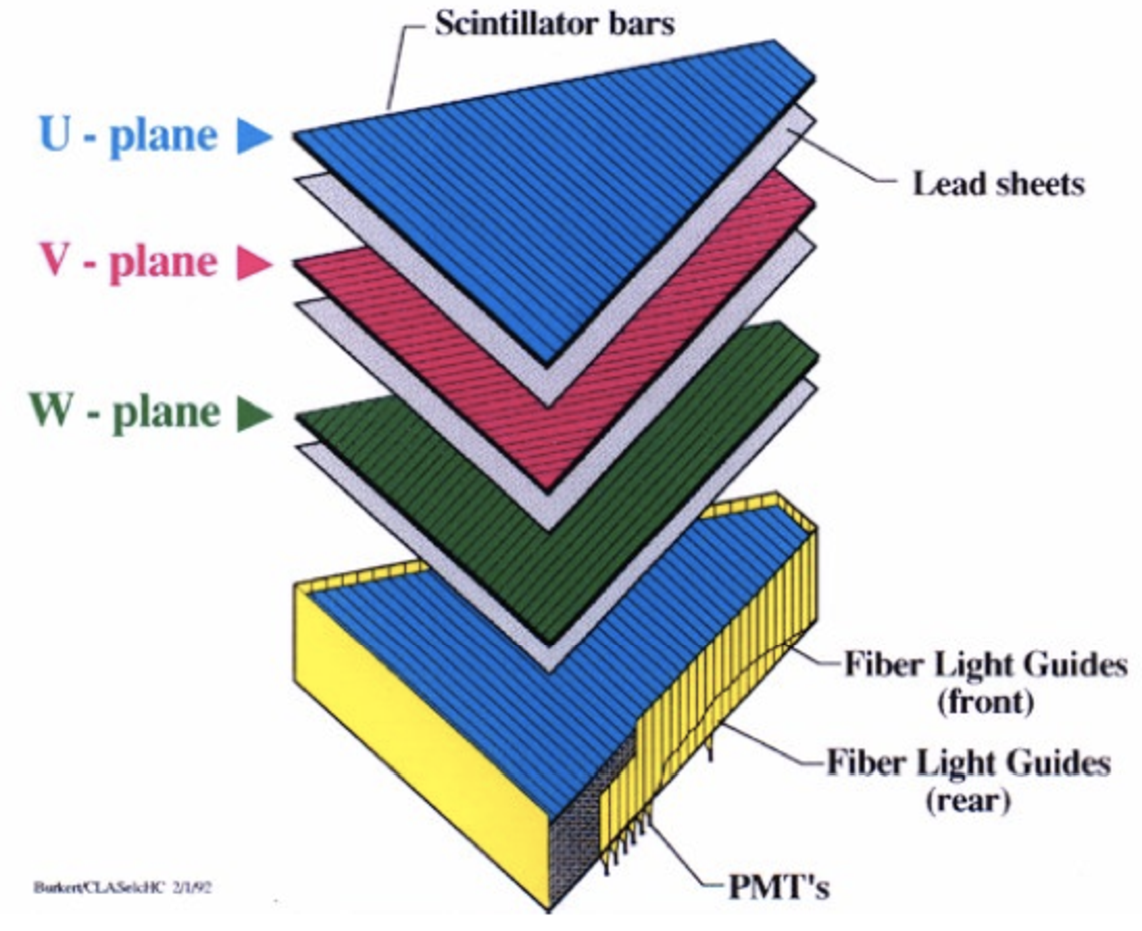
\includegraphics[width=0.8\columnwidth,height=0.75\hfigheight]{\figures/hall-b/CCECPLOTS/Calorimetry/CLASEC.pdf}\label{fig:clas.ec}
}

\subfloat[][]{
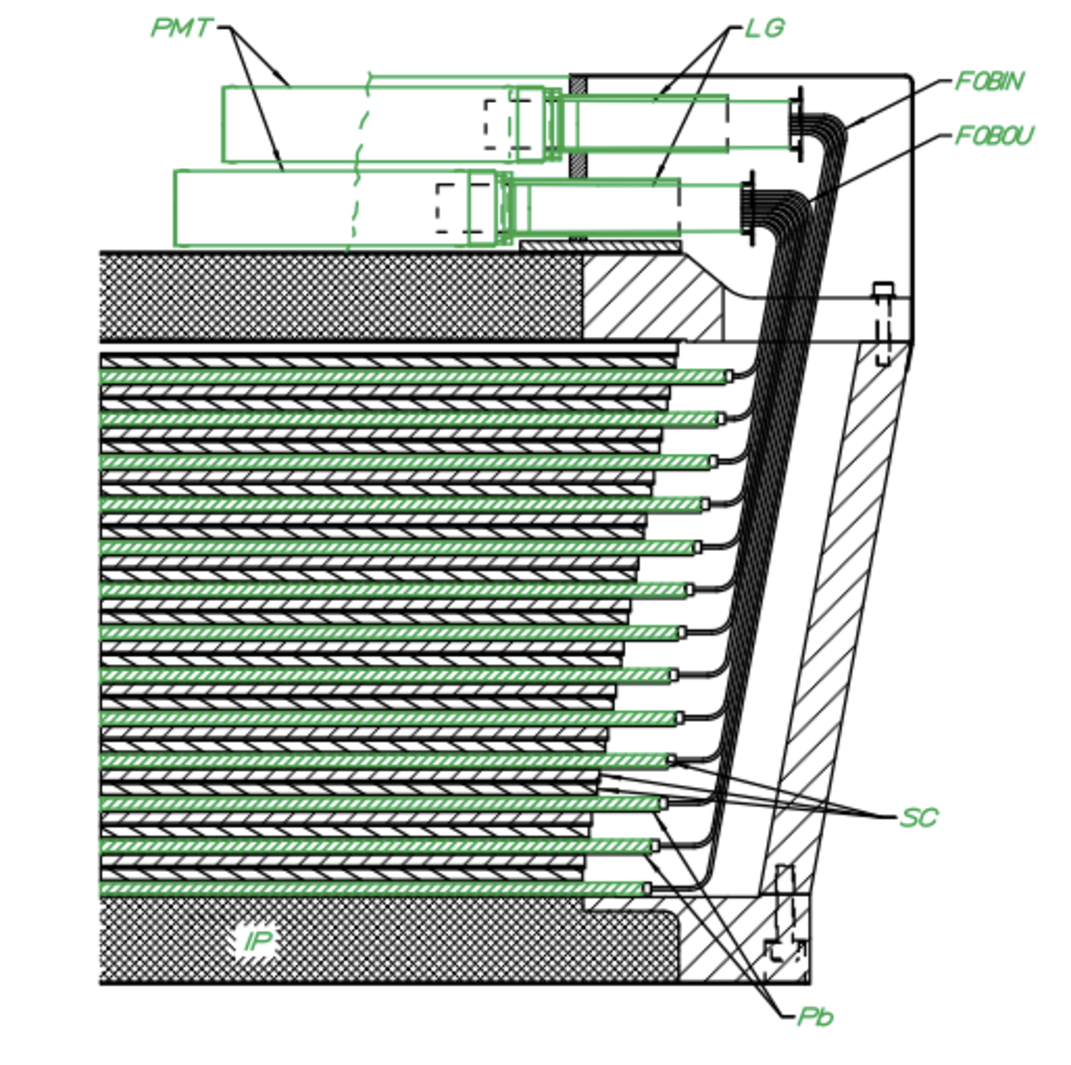
\includegraphics[width=0.8\columnwidth,height=0.75\hfigheight]{\figures/hall-b/CCECPLOTS/Calorimetry/CLASECSIDE.pdf}\label{fig:clas.ec.side}}
\caption[Separated view of one sector of the forward electromagnetic calorimeter (\abbr{EC}) showing the three planes ($u$, $v$, $w$) of scintillator-lead pairs which make up one of the 13 logical layers]{Separated view of one sector of the forward electromagnetic calorimeter (\abbr{EC}) showing the three planes ($u$, $v$, $w$) of scintillator-lead pairs which make up one of the 13 logical layers~(a). Side view of one plane of the forward electromagnetic calorimeter (\abbr{EC}) showing the the 13 logical layers, placement of the \abbr{PMT}'s and light guides~(b). Image Source: \subref{fig:clas.ec}~\cite{clas.ec} , \subref{fig:clas.ec.side}~\cite{clas.ec} respectively.} 

\end{center}\end{figure}

Using the three layers in each logical layer to provide pixel-like information, the transverse shower development for a given particle can be determined. All final-state photons were identified in the \abbr{EC} if no charged tracks have been associated with an energy deposit and also the velocity, $\beta$, of the particle exceeds 0.9c. Particles with $\beta <$~0.9c are neutron candidates.
%The difference in energy deposit between the inner and outer layers provides separation of electrons from pions in the reconstructed data for energies less than 2.8~GeV. For energies greater than 2.8~GeV, identification of pions and electrons are obtained by comparing the energy deposited in the \abbr{EC} with the momentum determined from the \abbr{DC}.
\section{Data Aquisition System}\label{sec:clas.daq}

The data acquisition system for the \abbr{CLAS} detector is composed of several layers of electronics. The amplified signals from the various wires and photo-multiplier tubes are received by the \abbr{TDC} and \abbr{ADC} counters. A certain set of these signals are used in the \emph{trigger} to determine if an event of interest has occurred. If it has, then all the signals are sent to the ``event builder'' via \abbr{CAMAC}\label{abbr:camac}\cite{clas} crates and recorded as a single event.

The controlling program makes use of the \abbr{CEBAF} On-line Data Acquisition System (\abbr{CODA}\label{abbr:coda})\cite{clas}. At the time of the \g12 experiment, the \abbr{DAQ} was capable of over 10~kHz. This high rate was due in part to a new field-programmable gate array \abbr{FPGA}\label{abbr:fpga} logic control processor that was integrated into the trigger system for \abbr{CLAS}\cite{clas.trig}.

The input components to the triggering system of \abbr{CLAS} are obtained from the tagger, time-of-flight, start counter, electromagnetic calorimeter and \v{C}erenkov counters. The \abbr{TOF} and \abbr{ST} are used to identify ``prongs,'' or charged tracks, at the trigger level. These composed by a coincidence of any one \abbr{TOF} hit in a given sector with any one \abbr{ST} hit in the same sector. Additionally, a coincidence between the \abbr{EC} and \abbr{CC} above certain thresholds was included as a lepton trigger. The various trigger \emph{bits} used by the system are discussed in Sec.~\ref{sec:data.trig}.

\begin{figure}\begin{center}
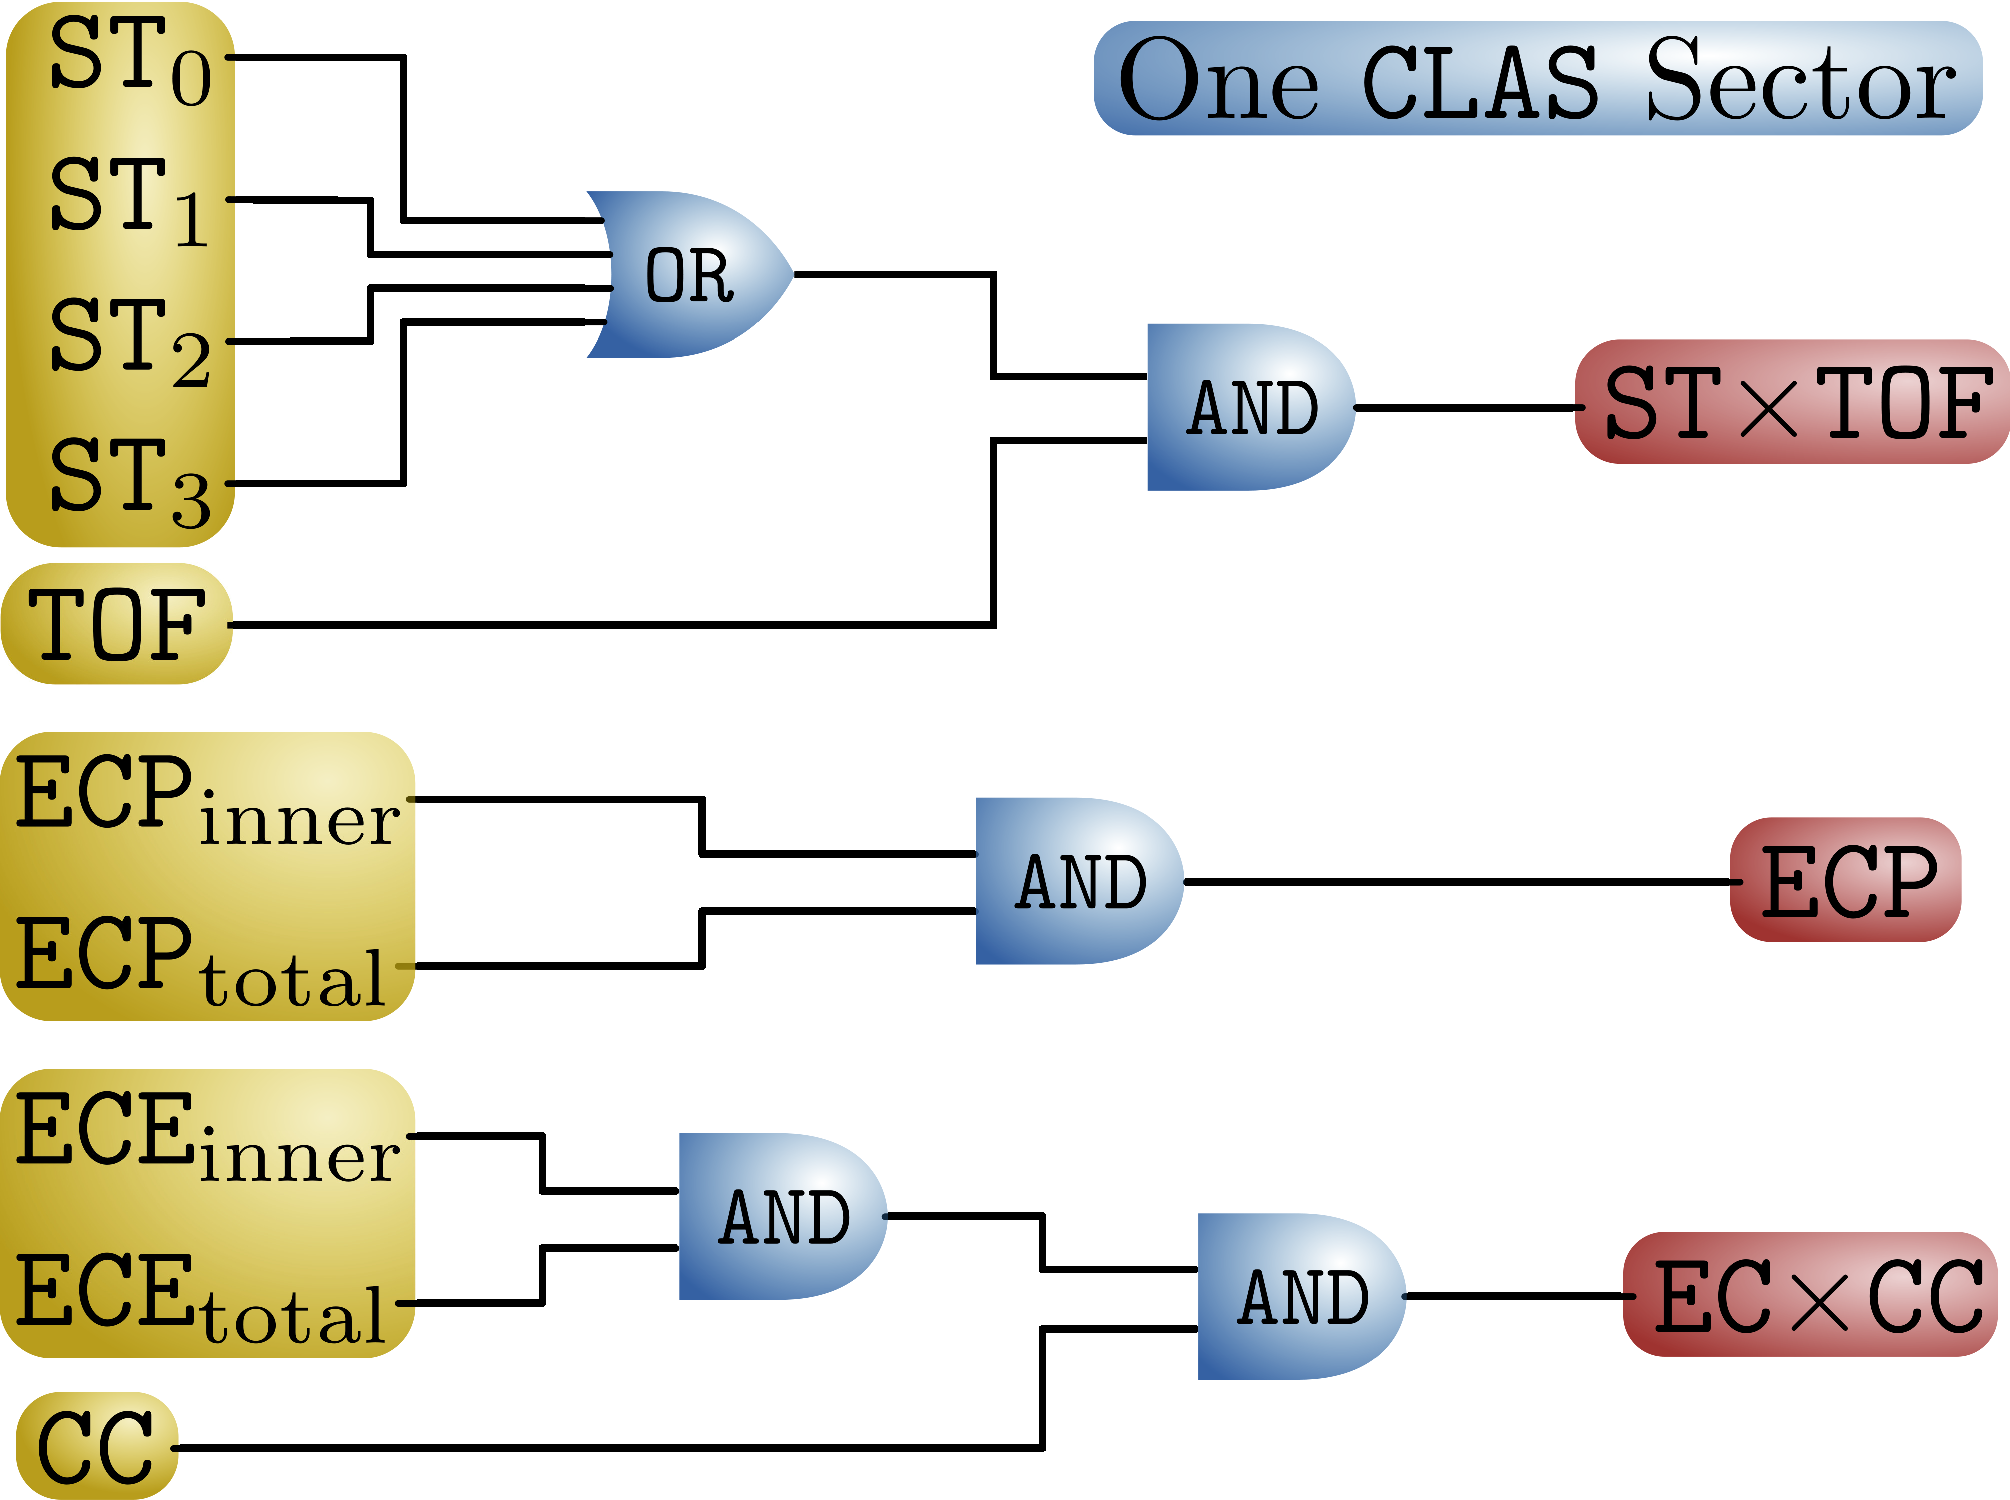
\includegraphics[width=0.8\figwidth]{\figures/hall-b/trigger_sector.pdf}
\caption[Trigger Logic - One Sector]{\label{fig:clas.daq.trigsec}{\coloronline}Trigger logic for one of the six sectors of \abbr{CLAS}. The \abbr{ST$\times$TOF} signal is a coincidence between any of the four start counter \abbr{TDC} signals (numbered from 0 to 3) and any of the 57 \abbr{TOF} \abbr{TDC} signals. The \abbr{ECE}$_\mathrm{inner}$ and \abbr{ECE}$_{\mathrm{total}}$ are the \emph{electron}-threshold \abbr{EC} signals for the energy deposited in the \emph{inner} layer and in \emph{all} layers. These are combined with a \abbr{CC} signal to produce the \abbr{EC$\times$CC} trigger for this sector. The \abbr{ECP} trigger signal is the \emph{photon}-threshold \abbr{EC} signal. These trigger signals are discussed further in Sec.~\ref{sec:data.trig}.}
\end{center}\end{figure}

\section{The \g12 Experiment}\label{sec:clas.g12}

briefly explain the need of \g12

\subsection{\g12 Running Condtions}\label{sec:clas.g12.conditions}

explain \g12, use proposals for this

\subsection{G12 Data Acquisition \& Reconstruction }\label{sec:clas.g12.conditions.data}

Explain g12 data retrieval

\subsection{\g12 Corrections}\label{sec:clas.g12.corrections}

lets write about the beam corrections that were needed because of hysteresis and also the efficiency corrections needed for ''normalization" 
%
%Three \abbr{CLAS} analysis proposals (\abbr{04-005}\cite{clas.proposal.hyclas}, \abbr{04-017}\cite{clas.proposal.superg} and \abbr{08-003}\cite{clas.proposal.pion}) defined the experimental and theoretical basis for the \g12 running period. \label{sec:clas.hyclas}The \abbr{04-005} experiment, \emph{Search for New Forms of Hadronic Matter in Photoproduction}, also called \abbr{HyCLAS}, had a meson spectroscopy focus with multiple charged particle final states such as
%\begin{eqnarray}
%    \gamma \p & \rightarrow & \p \pi^+ \pi^- \pi^0, \\
%    \gamma \p & \rightarrow & \n \pi^+ \pi^+ \pi^-, \\
%    \gamma \p & \rightarrow & \p \Kp \Km \eta, \\
%    \gamma \p & \rightarrow & \n \Kp \Kp \pi^-, \\
%    \gamma \p & \rightarrow & \Delta^{++} \eta \pi^-, \\
%    \gamma \p & \rightarrow & \p \p \bar{\p}.
%\end{eqnarray}
%The physics involved with \abbr{HyCLAS} required the configuration of \abbr{CLAS} to provide the largest acceptance for these multiple particle final states. Phase-space generated events of $\mathrm{\gamma p \rightarrow p \pi^+ \pi^- \pi^0}$ were simulated (see page~30 of \cite{clas.proposal.hyclas}) with the $t$-slope obtained from the \textit{g6c} experiment. The primary requirement for the greatest acceptance of such events was to have the target up-stream (see Sec.~\ref{sec:clas.tgt}) of the normal position at the ``center'' of \abbr{CLAS}. This target placement gave better acceptance for particles close to the beam-line but sacrificed large momentum-transfer events where the final state particles were more than about 70$^\circ$ away from the beam-line.
%
%\label{sec:clas.superg}The \abbr{04-017} experiment, \emph{Study of Pentaquark States in Photoproduction off Protons}, also called \abbr{Super-G}, was founded on a search for the $\Theta^+$ and $\Xi^{--}_{5}$, so-called \emph{penta-quarks}, as well as a study of the ``conventional'' $\Xi$ spectrum (see page~16 of \cite{clas.proposal.superg}.) This analysis is part of the latter topic. The running requirements were similar to that of \abbr{HyCLAS} with the need for a higher energy beam. An examination of the ground state $\Xi^-$ reaction:
%\[
%    \mathrm{\gamma p \rightarrow \Xi^- K^+ K^+},
%\]
%provides a starting point for this analysis. The threshold energy of the incident photon ($E_\gamma$) is given by
%\begin{equation}
%    E_{\gamma} = \frac{m_{\Xi}^2 + 4 m_{\mathrm{K}}^2 + 4 m_{\rule{0pt}{1.4ex}\Xi} m_{\rule{0pt}{1.4ex}\mathrm{K}} - m_{\p}^2}{2 m_{\p}},
%\label{eqn:xi.threshold}
%\end{equation}
%where $m_{\rule{0px}{1.4ex}\Xi}$ is the mass of the $\Xi$, $m_{\rule{0px}{1.4ex}\mathrm{K}}$ is the mass of the K$^{+}$, and $m_{\p}$ is the proton (target particle) mass. For the ground state $\Xi(1320)$ which has a mass of 1.322~GeV, the threshold energy $E_\gamma$ is 2.4 GeV. Since the beam
%(photon) and the target (proton) are both known quantities, we can measure the two kaons and calculate the $\Xi^-$ through ``missing mass'' which is discussed in detail in Chapter~\ref{sec:analysis}. There is a minimum transverse momentum the final state particles must have to be measured by \abbr{CLAS}, otherwise they would travel right down the beam line. Therefore, in order to detect the two kaons with \abbr{CLAS}, a photon energy approximately 0.5~GeV above threshold is required. This corresponds to 2.9~GeV in the reaction for the ground state $\Xi(1320)$.
%
%The third proposal, \abbr{08-003}, titled \emph{The $\gamma \p \rightarrow \pi^+ \n$ Single Charged Pion Photoproduction}, was approved just before the \g12 run period started. This was added onto \g12 as part of the physics to be done with the data collected. It required a single track trigger (see Sec.~\ref{sec:data.trig} on page~\pageref{sec:data.trig}) and lower current. This configuration allowed the data from these special runs to be included in analyses of the ``production'' \g12 data set.
%
%At the beginning of \g12 run, approval came for purchasing gas for the \v{C}erenkov subsystem of \abbr{CLAS}; see Sec.~\ref{sec:clas.cc}. The \v{C}erenkov counters were filled and turned on two weeks into the running period enabling the separation of electons from pions. As a result, a whole new set of leptonic physics became available in what was already a very rich data set.



%\section{Electron Accelerator} \label{sec:clas.acc}

The \abbr{CEBAF} electron accelerator is able to deliver a 75\% polarized electron beam of up to approximately 6~GeV to each of the three halls simultaneously. The beam as seen by each hall consists of clusters of electrons separated by approximately 2~ns. Typical intensities for halls \desg{A} and \desg{C} are 10--100~\text{$\mu$} A, however, due to the nature and sensitivity of the \abbr{CLAS} detector, beam currents to hall \desg{B} are typically 10--100~nA.

Using a GaAs photocathode laser driven gun system, a highly polarized electron beam is produced and accelerated through a radio-frequency (\abbr{RF}) chopping system operating at 499~MHz. The three-beam, 1497~MHz ``bunch train'' at 100~keV is then longitudinally compressed and accelerated to just over 1\% of the total machine energy before it is injected into the first main accelerator. This compression results in a beam of 2~ps bunches separated by 668~ps.

The main accelerator consists of a pair of linear accelerators (\abbr{LINAC}s\label{abbr:linac}) which consists of twenty cryomodules each containing eight superconducting niobium cavities as shown in Fig.~\ref{fig:jlab.cavity}. This was the first use of superconducting cavities and marked a major advancement in the field of accelerators. Prior to the \abbr{CEBAF} breakthrough, typical accelerating cavities used non-superconducting metals like copper whose resistivity would cause a build up of heat. The niobium superconducting cavities are kept at 2~Kelvin and are non-resistive, eliminating the heating problems of copper. The significant cooling requirements are satisfied by the Lab's Central Helium Liquefier (\abbr{CHL}\label{abbr:chl}).

\begin{figure}\begin{center} 
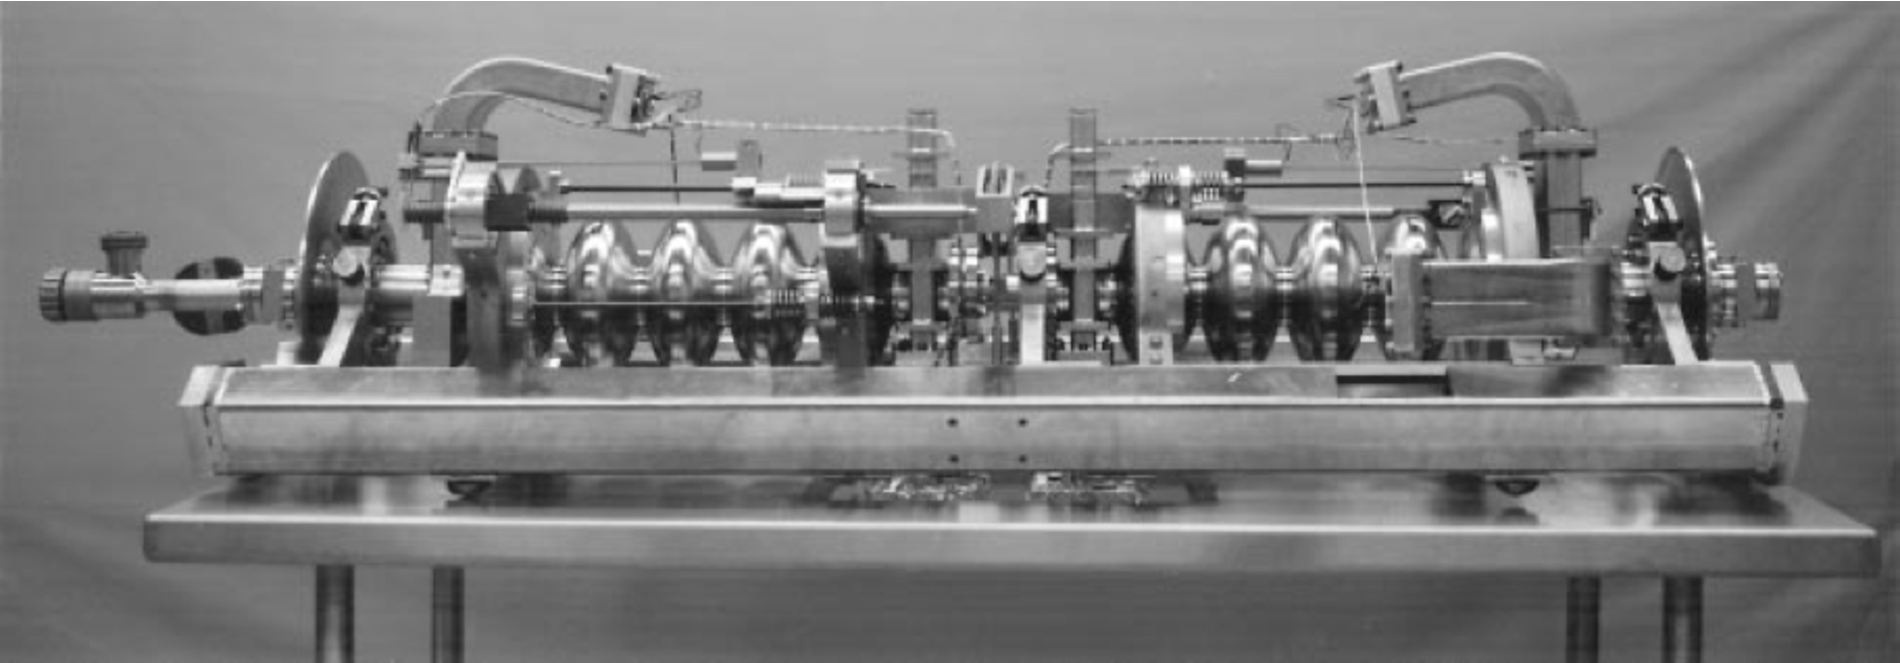
\includegraphics[width=\figwidth]{\grpath/jlab/niobium_cavity_pair.pdf}
\caption[Niobium Cavity Pair (photograph)]{\label{fig:jlab.cavity}A superconducting niobium cavity pair. These devices are tuned for specific energy resonances by mechanically adjusting their lengths on the order of a few micrometers.}
\end{center}\end{figure}

A standing electromagnetic wave is induced inside the niobium cavities as shown in Fig.~\ref{fig:jlab.accel} and the electrons passing through experience a continuous acceleration. Before \abbr{CEBAF}, the copper accelerating cavities used were tuned by adjusting the cooling system. The resistivity of the copper would cause the cavity to heat up and expand and the cooling system would be set so the desired length was obtained. The superconducting niobium cavities on the other hand are non-resistive and do not heat up. Therefore, the cavities are lengthened or shortened mechanically (on the order of a few micrometers) to tune the wavelength and maximize the acceleration of the electrons.

\begin{figure}\begin{center}
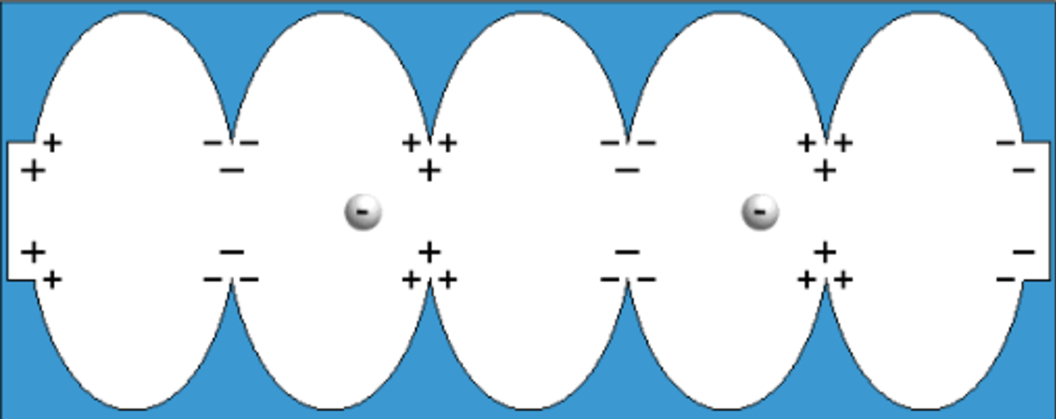
\includegraphics[width=0.8\figwidth]{\grpath/jlab/accelerating_diagram.pdf}
\caption[Accelerating Cavity Diagram]{\label{fig:jlab.accel}As the electron clusters travel through a superconducting niobium cavity, shown in Fig.~\ref{fig:jlab.cavity}, they experience a continuous acceleration due to a standing electromagnetic wave indicated by the positive and negative signs along the inner wall.}
\end{center}\end{figure}

The \abbr{LINAC}s are connected by two sets of 180$^\circ$ magnetic-dipole bending arcs (see Fig.~\ref{fig:jlab.cebaf}) with a radius of 80~meters. The beam is sent through both accelerators and is then \emph{recirculated} up to four more times. Each \abbr{LINAC} is capable of accelerating the beam by up to 600~MeV giving approximately 1.2~GeV per pass. A plan to nearly double the energy of the beam was approved by \abbr{DOE}\label{abbr:doe} and the 12~GeV program started construction on September 15, 2008\cite{jlab.news.cd3, jlab.12gev.starts}.

The beam is selectively extracted using \abbr{RF} cavities tuned to 499~MHz --- the frequency dictated by the manufactured geometry. By slightly accelerating every third bunch, while not disturbing the other two, the electrons are bent out of the recirculating \abbr{LINAC} and sent to one of the halls. Each of the first four passes can be delivered to only one hall at a time, however the fifth (final) pass can be sent to all three halls simultaneously. The 499~MHz extraction creates the final beam as seen by the hall which consists of $\sim2$~ps bunches separated by 2.004~ns. At the time of the \g12 experiment, the accelerator was capable of delivering a maximum electron beam energy of 5.7~GeV. The tagger subsystem (see Sec.~\ref{sec:clas.tagr}) tagged photons of energies up to 95\% of the delivered beam, and therefore the maximum energy photon seen in \g12 was 5.4~GeV.

%\FloatBarrier
\section{Beam Positioning}\label{sec:clas.beam}
%\FloatBarrier
There are several beam monitoring stations in Hall \desg{B} before and after the \abbr{CLAS} detector (Fig.~\ref{fig:clas.beam.beforemonitors}) to scan the important details of the electron beam prior to conversion into a photon beam and the details of the photon beam before and after entering the target. Such quantities for the electron beam include position, intensity, dispersion, and current, and for the photon beam include position, dispersion and flux. Most of these monitoring stations are used by the accelerator group.
% to steer the beam to the target as they control all magnets that can substantially move the beam.
\begin{figure}[h!]\begin{center}
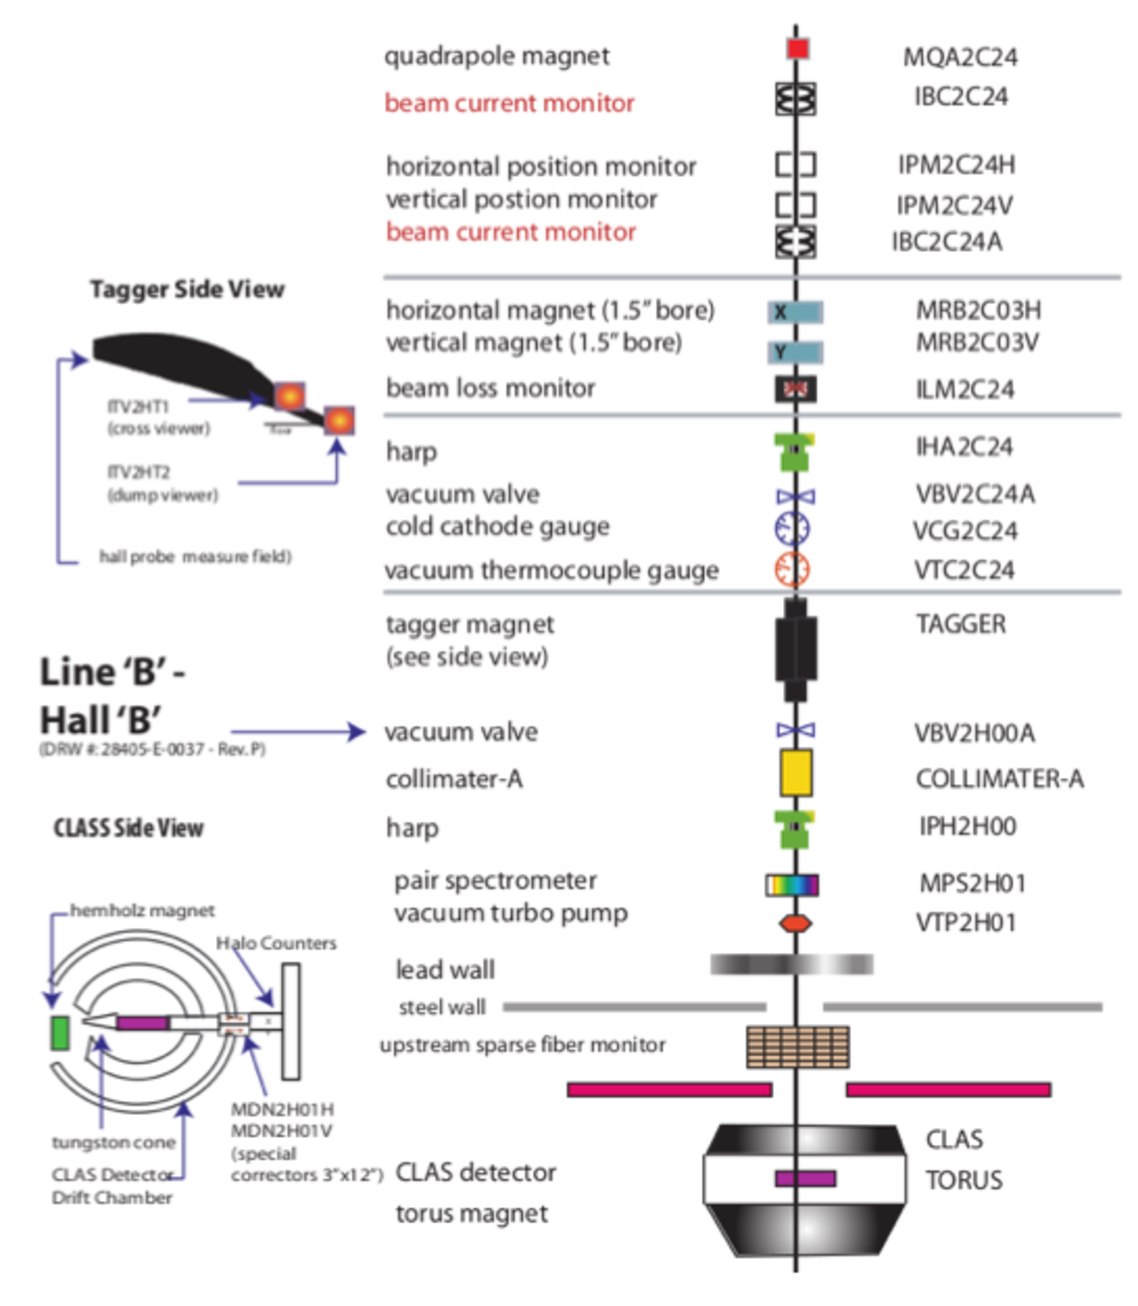
\includegraphics[width=\figwidth, height=1.75\hfigheight]{\grpath/hall-b/beamline_components.pdf}
\caption[Beamline and components of \abbr{CLAS}]{\label{fig:clas.beam.beforemonitors}{\coloronline}Beamline and components of \abbr{CLAS}. Image Source~\cite{cebafflckr}}
\end{center}\end{figure}
There are two types of devices to measure the electron beam position. The first type is represented by two beam position monitors (\abbr{BPM}s\label{abbr:bpm}) placed before the tagger. The position monitors use three radiofrequency cavities to measure the transverse location of the electron beam and its intensity. This information is used as feedback for the steering mechanism. The position monitors are noninvasive and measure at a rate of 1 Hz. 
The second type of device used to measure the beam position is the Harp Beam Profile Monitor, which also measures the electron beam dispersion. The harp devices consist of fine wires (20 and 50~{\um} W and 100~{\um} Fe) that can be passed through the beam at specific orientations and collect scattered electrons with a photomultiplier tube. This procedure measures the horizontal ($x$) and vertical ($y$) profile of the electron beam and is performed after any downtime or change in the beam. The accelerator group adjusts the beam position such that more than 99\% of the electron beam goes through the radiator. Since this process is invasive, it was only done when the drift-chambers and \abbr{DAQ} were turned off. A harp scan measurement for \g12 is shown in Fig.~\ref{fig:clas.beam.harpscan}. The width of the beam was contained within a 200 $\mathrm{\mu}$m diameter.



%\begin{figure}\begin{center}
%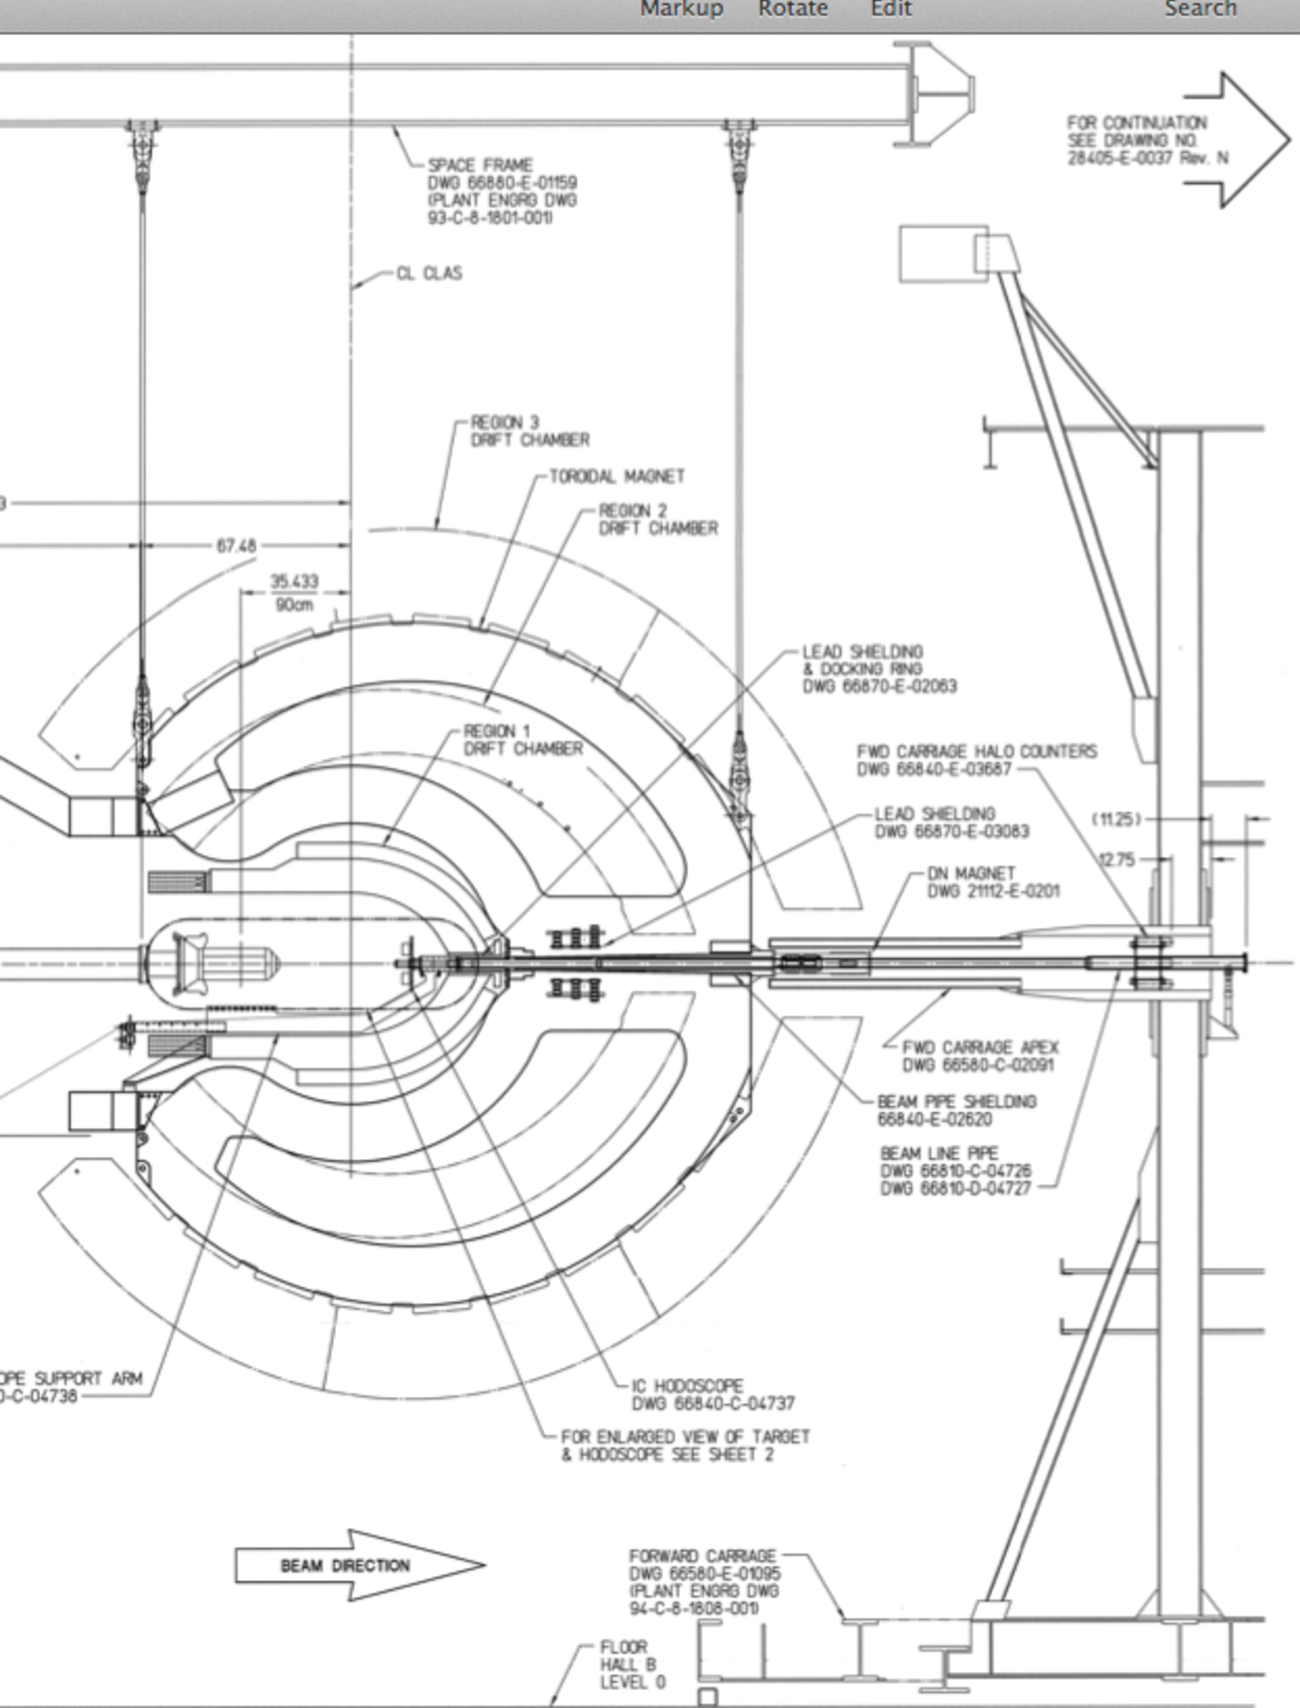
\includegraphics[width=\figwidth,height=\hfigheight]{\grpath/hall-b/G12_afterbeam_blueprint.pdf}
%\caption[Beamline and \abbr{CLAS} components in \g12]{\label{fig:clas.beam.aftermonitors}{\coloronline}Beamline and \abbr{CLAS} components in \g12}
%\end{center}\end{figure}

\begin{figure}\begin{center}
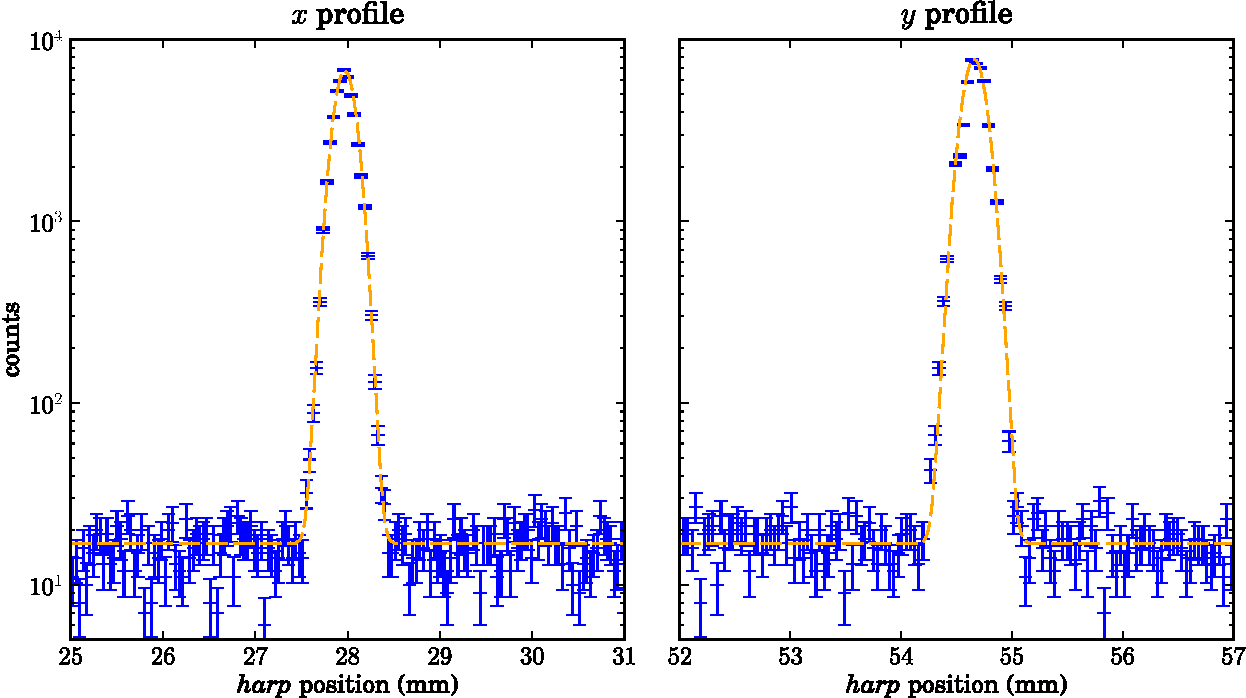
\includegraphics[width=\figwidth,height=\qfigheight]{\grpath/calibration/harpscan.pdf}
\caption[A typical \emph{harp} scan done just prior to run 56426]{\label{fig:clas.beam.harpscan}{\coloronline}A typical \emph{harp} scan done just prior to run 56426. Shown are the $x$ and $y$ profiles of the electron beam just before the tagger. The dashed orange line is a Gaussian fit to the data: $\sigma_x~=~0.115$~mm and $\sigma_y~=~0.105$~mm. Image Source:~\cite{goetz}}
\end{center}\end{figure}

The Total Absorption Shower Counter located downstream of \abbr{CLAS}, measures the photon flux (see Fig.~\ref{fig:clas.beam.afterCLAS}). The \abbr{TASC}, consists of four lead glass blocks of $\sim$ 17 radiation lengths, each coupled to a photo-multiplier tube (\abbr{PMT}\label{abbr:pmt}). The \abbr{TASC} is approximately 100\% efficient at detecting photons at beam currents less than 100~pA\cite{clas.tagger,clas.tagger.calib}. Since \g12 ran with 65~nA current, special low current, 50~pA, normalization runs(see Table~\ref{tab:data.calibruns}) were taken several times throughout \g12. The ratio of electrons detected in the photon tagger (see Sec.~\ref{sec:clas.tagr}) to that of photons detected in the \abbr{TASC} gives the tagging ratio used to calibrate the tagger and measure the flux throughout the entire \g12 run period.
%with hits in the left and right \abbr{TDC} matching in time and a corresponding hit in an E-counter
\begin{figure}[h!]\begin{center}
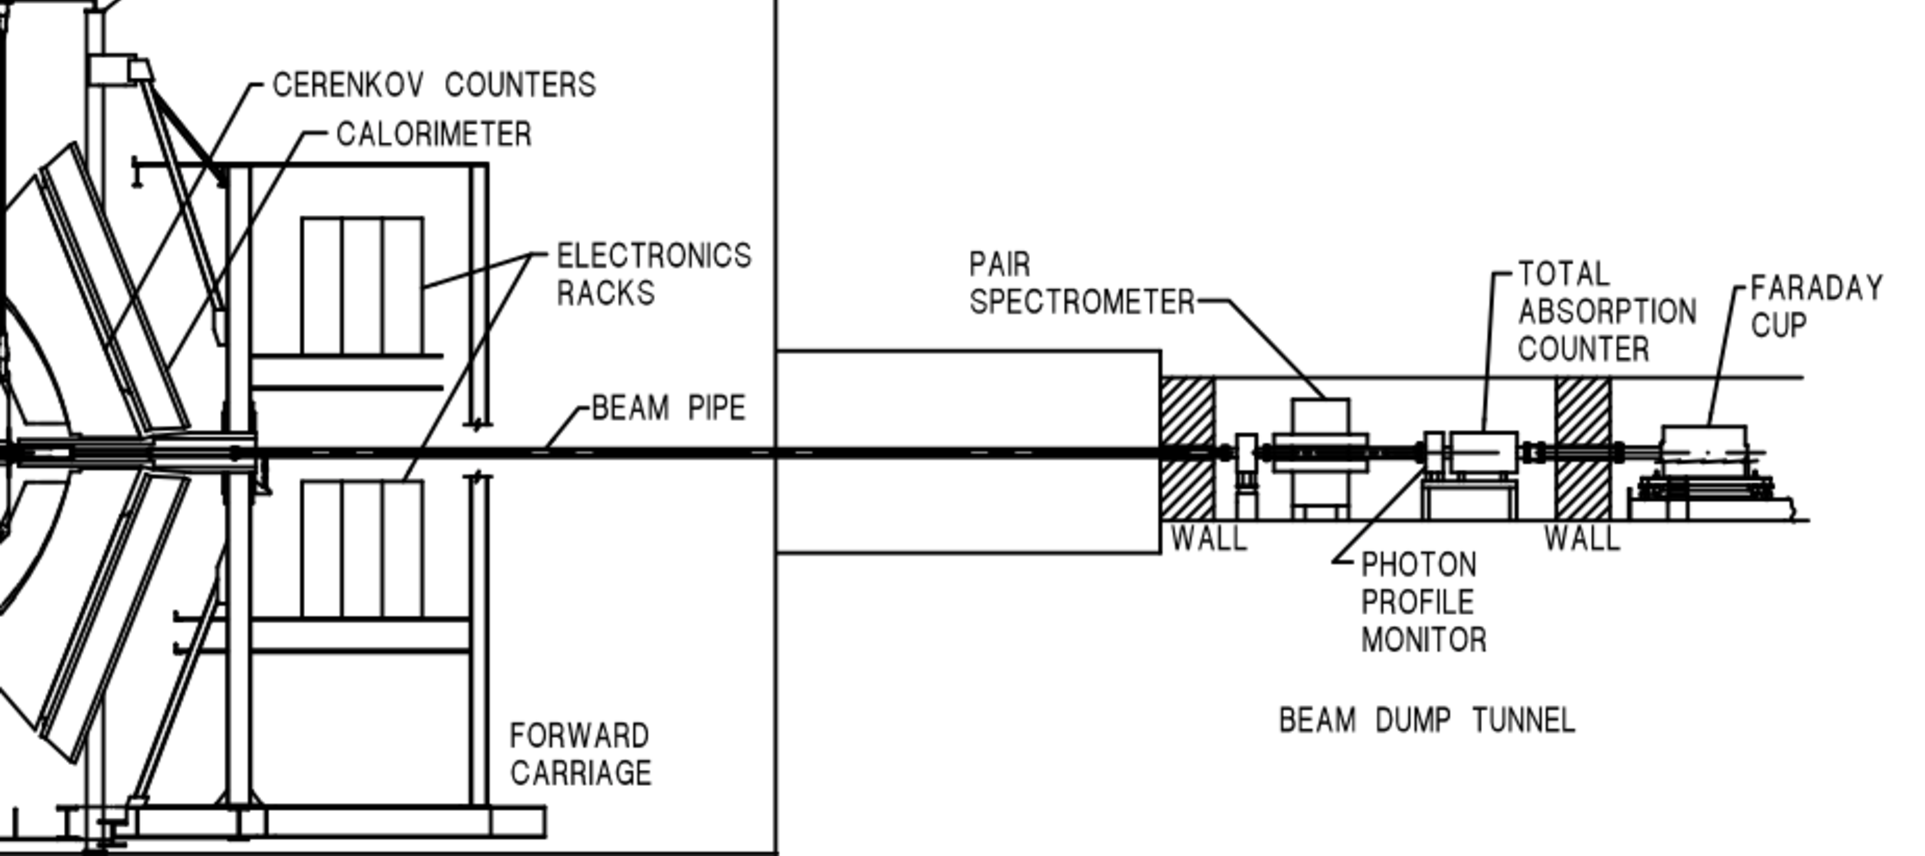
\includegraphics[width=\figwidth,height=0.8\qfigheight]{\grpath/hall-b/TASC_blueprint.pdf}
\caption[Beamline and components after \abbr{CLAS} ]{\label{fig:clas.beam.afterCLAS}{\coloronline}Beamline components in \g12 after \abbr{CLAS}}
\end{center}\end{figure}

\FloatBarrier
%\section{Photon Tagger} \label{sec:clas.tagr}

The electron beam delivered to hall \desg{B} from \abbr{CEBAF} can be sent directly to a target or the electron beam can produce a \emph{real photon} beam by means of bremsstrahlung radiation by passing the electron beam through a radiator. Typical radiators have high atomic number to help reduce contamination of photons produced by electron-electron scattering. The \g12 experiment used a gold (\abbrlc{A}{u}) foil of $10^{-4}$~radiation length. This choice has a double purpose, to maximize the probability of the electron-nucleus interaction given that the bremsstrahlung cross section is proportional to $\mathrm{Z^{2}}$, and to minimize the number of interaction centers such that each electron interacts once, producing only one photon. After the electron beam passes through the radiator, the beam becomes a mixture of photons and electrons that did not interact with the radiator and recoil electrons. The mixed beam then travels into a dipole magnetic field which sweeps the electrons out of the electron-photon beam. The electrons present in the electron-photon beam are directed toward two hodoscope planes, each made of an overlapping array of scintillators to detect the energy-degraded electrons.

%  

The first scintillator plane, referred to as the E-plane (Figs.~\ref{fig:jlab.tagr.energies}, and~\ref{fig:jlab.tagr.paddles}), is used to determine the momentum of the recoiling electrons. The E-plane provides photon energy resolution on the order of 0.1\% of the incident electron beam energy. It consists of 384 paddles that are 20 cm long, 4 mm thick and from 6 to 18 mm wide. The paddles are arranged in an overlapping fashion, thus increasing the number of logical paddles to 767.
The trajectory of an electron or any charged particle in the magnetic field is governed by the equation
\begin{equation}\label{eq:motioninmag}
	p = qrB \ (\mathrm{if}\ \vec{p} \perp \vec{B} )
\end{equation}
where $p$ is the particle's momentum, $q$ is the particle's charge, $r$ is the particle's radius of curvature and $B$ is the magnetic field the particle passes through.
By determining which paddle an electron hit we know the radius of curvature and we can calculate the momentum of the electron. The momentum of the electron can then be used to obtain the energy of the photon by means of the conservation relation 
\begin{equation}\label{eq:tagger.energy}
	E_{\gamma} = E_{0} - E_{e}
\end{equation}
where $E_{0}$ is the energy of the incident electron given by \abbr{CEBAF}, $E_{e}$ is the energy of the recoil electron and $E_{\gamma}$ is the energy of the emitted photon. 

The second scintillator plane, referred to as the T-plane, is used to make accurate timing measurements of the recoiling electrons. This plane comprises of 61 paddles that are each 2 cm thick. The added thickness of these paddles allow for a timing resolution of 110 ps.
% The spectrometer was able to tag photons ranging from 20-95\% of the incident electron beam energy.

The tagger can tag photons of energies from 20 to 95\% of the incident electron beam energy. For \g12 this corresponds to a photon energy range of 1.142 - 5.425~GeV. Due to the high current of the electron beam delivered to \g12 from \abbr{CEBAF} there were usually more than one ``hit'' in the tagger for each event. Normally, the one associated with the photon that caused the event could be obtained by a timing coincidence with the tracks, although there are cases when this photon is ambiguous as discussed in Sec.~\ref{sec:analysis.beam}.

The photons that pass through the radiator then pass through a 6.2~mm diameter collimator. Collimation is used to trim the beam halo prior to arriving at the CLAS cryotarget. In the \g12 experiment the beam entering the cryotraget was 1.5~cm in radius. The collimator was positioned 537~cm upstream of the cryotarget which had a radius of 2~cm. A sweeping magnet were placed after the collimator to remove any charged particles created by interactions of photons with the collimator.

More detailed information on the Hall B tagging system and \abbr{DAQ} of the tagger system can be found in \cite{clas.tagger}.

\begin{figure}\begin{center}
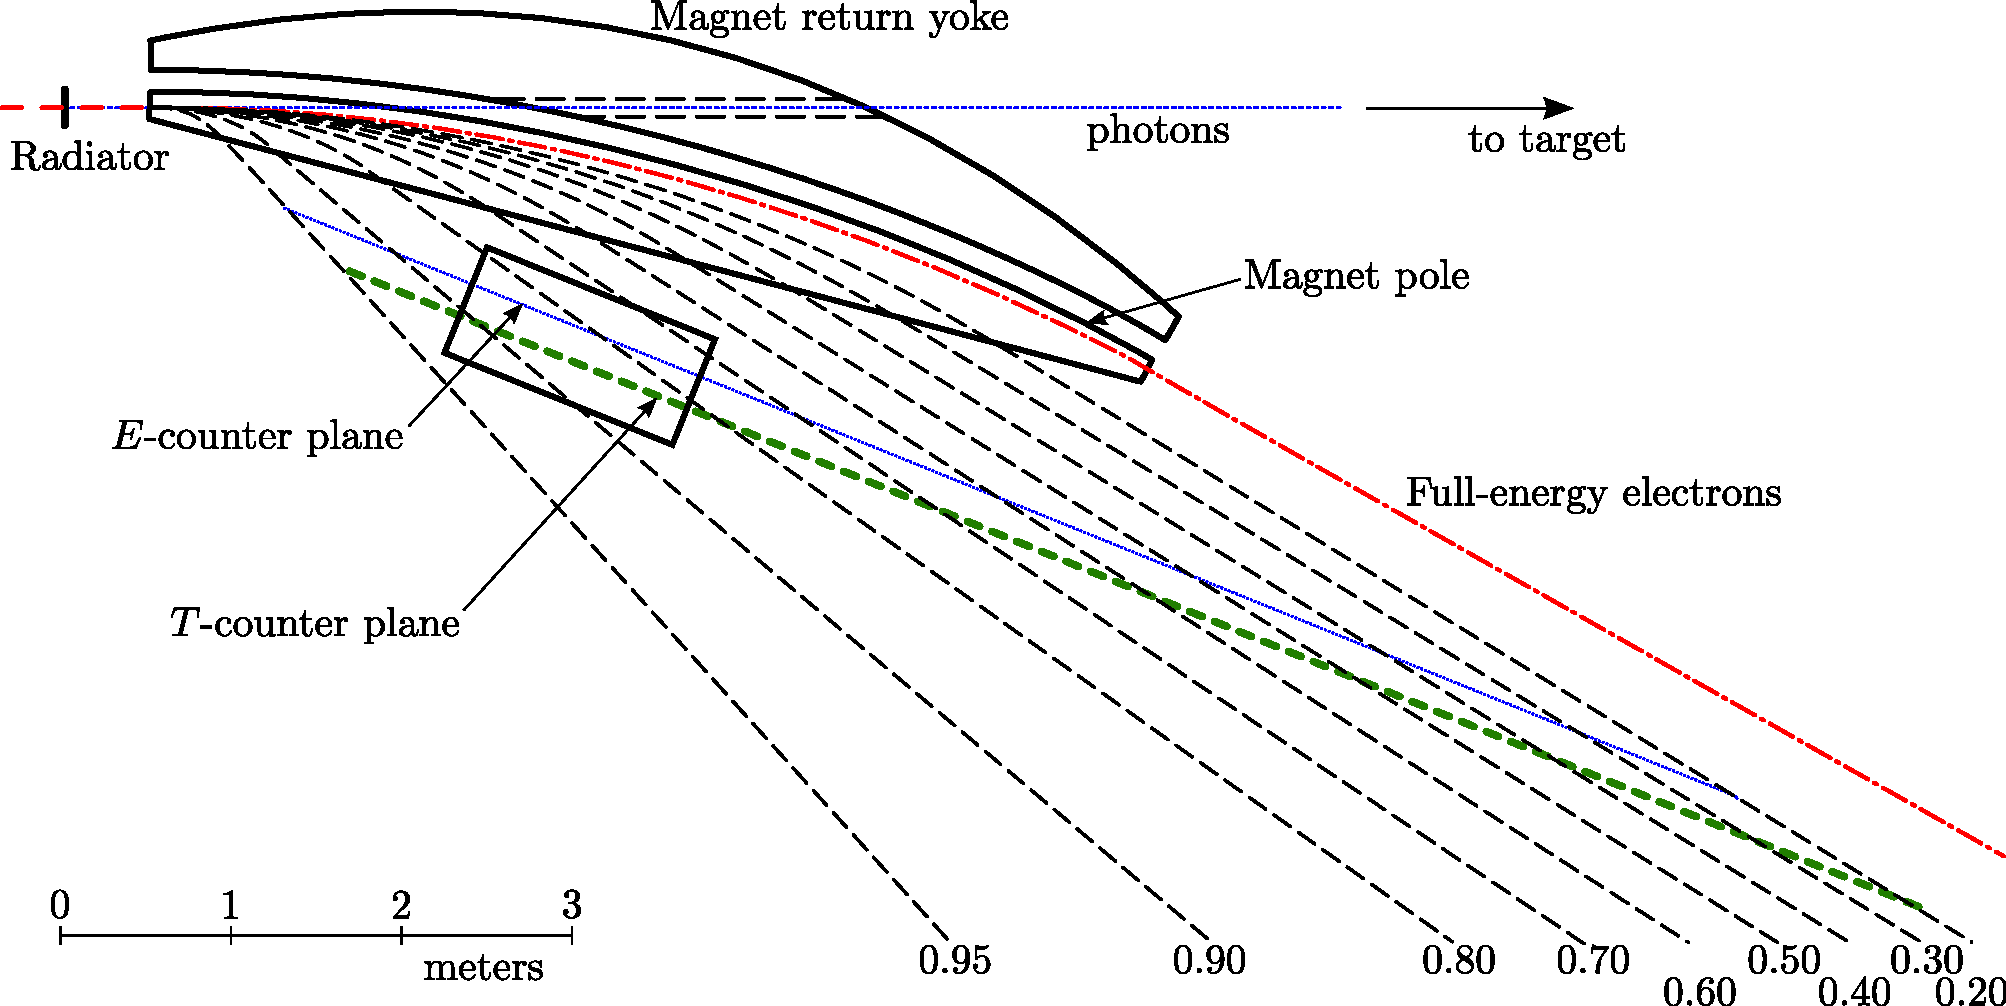
\includegraphics[width=0.8\figwidth,height=\qfigheight]{\grpath/hall-b/tagger_energies.pdf}
\caption[Scale drawing of the photon tagger system]{\label{fig:jlab.tagr.energies}Scale drawing of the photon tagger system. The rectangular area around the $E$ and $T$-counter planes outlines the expanded view shown in Fig.~\ref{fig:jlab.tagr.paddles}.}
\end{center}\end{figure}


\begin{figure}\begin{center}
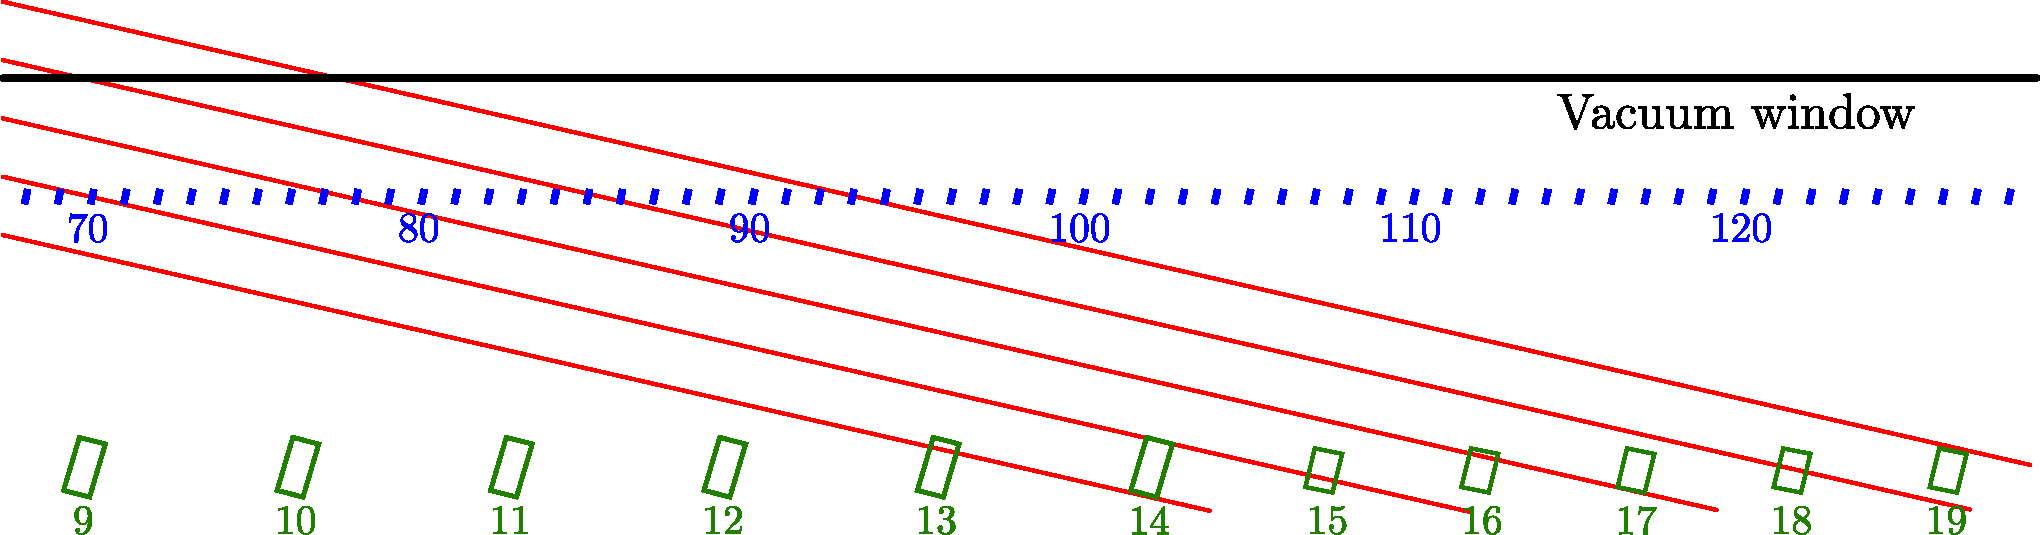
\includegraphics[width=1.1\figwidth,height=\qfigheight]{\grpath/hall-b/tagger_paddles.pdf}
\caption[Scale drawing of the $E$-counters (blue) and the $T$-counters (green) showing examples of recoiled electrons (red lines) entering from the upper left]{\label{fig:jlab.tagr.paddles}{\coloronline}Scale drawing of the $E$-counters (blue) and the $T$-counters (green) showing examples of recoiled electrons (red lines) entering from the upper left.}
\end{center}\end{figure}
\FloatBarrier

%%\section{\label{sec:clas.sh}Scintillator Hodoscope (\abbr{SH})}

\todo{NOTE: This section might have to wait (or be cut) untill we actually start using the SH.}

New to \abbr{CLAS}, and installed after the second week of running \g12, was a scintillator hodoscope (\abbr{SH}) placed a few centimeters downstream of the target. This consisted of square ``pixels'' which were read out via silicone photo-counters (\abbr{ScPMC}). This was added in anticipation of the following runs which would use it as a veto counter for the inner calorimeter.




%The CEBAF Large Acceptance Spectrometer (CLAS) was used to detect particles produced by interactions of the photon beam with the cryogenic target located near the center of the CLAS de- tector. The main CLAS subsystems are the start counter, drift chambers, time-of-flight scintillators, along with Cerenkov counters and electromagnetic calorimeters in the forward region. The latter two forward region detector elements were not used in our analysis and will not be discussed here. Our analysis did not incorporate the start counter; however, it was used in the g11a trigger. The drift chambers were used to track charged particles, which were bent by a superconducting toroidal magnetic, as they traveled through the detector. By reconstructing a particle’s flight path, we were able to determine its momentum. The time-of-flight scintillator walls were used for particle identifi- cation purposes. In this section, we will discuss in detail the detector subsystems which played vital roles in our analysis.



%In Hall \desg{B} of \abbr{JLab}, the \abbr{CEBAF} Large Angle Spectrometer (\abbr{CLAS}\label{abbr:clas}) is, in essence, a large acceptance multi-wire proportional drift-chamber (\abbr{DC}). The main purpose of the \abbr{DC} in conjunction with the toroidal magnetic field (see Sec.~\ref{sec:clas.dc}) is to measure the momentum of charged final-state particles that leave the target. For the most part, the rest of the \abbr{CLAS} detector is used to obtain accurate timing and particle identification. In particular, a photon tagger, specific to Hall \desg{B} \emph{photon runs} as discussed in Sec.~\ref{sec:clas.tagr}, is used to measure the energy of photons incident on the target. In addition, there are several beam intensity and dispersion measuring devices used as described in Sec.~\ref{sec:clas.beam}.


%The physics program at \abbr{CLAS} investigates many aspects of nuclear and particle physics including but not limited to, transition form factors, medium modifications of meson propagation, short-range correlations in the nuclear medium, spin structure of the nucleon and spectroscopy of excited states. To study such mentioned physics with high statistical sensitivity and high detection efficiency, a large acceptance detector is required.

%The design of CLAS is based on a toroidal magnetic field generated by six superconducting coils made of niobium titanium alloy (NbTi) kept at 4.5 K by a recirculating helium flow. The direction of the toroidal field points along $\phi$ such that the charged particles conserve their azimuthal angle along their trajectory, except near the coils, which lies in the plane containing the beam axis. The kidney shape of the magnet was designed to provide a strong field gradient for the forward going particles carrying high momentum and a lower field gradient for particles emitted at larger angles (Fig. 2.3). At the maximum current of 3860 A the integral magnetic field reaches 2.5 T·m in the forward direction, dropping to 0.6 T·m at a scattering angle of 90◦. Another magnet used in CLAS is mini torus. Placed between the target and the first region of drift chambers, it reduces the background produced by scattered Moller electrons.

%The six coils separate CLAS naturally into six independent tracking areas (or sectors). The particle leaving the target crosses (Fig. 2.2) three regions of drift chambers (DC) which provide a measurement of a charged particle trajectory in the toroidal field, Cˇerenkov counters (CC) provide identification and separation of particles carrying the same charge, scintillator counters which measure the time of flight (TOF), and finally the electromagnetic calorimeters (EC) measures energy and enables detection of neutral particles.